%%%%%%%%%%%%%%%%%%%%%%%%%%%%%%%%%%%%%%%%%%%%%%%%%%%%%%%%%%%%%%%%%%%%%%
% Template for a UBC-compliant dissertation
% At the minimum, you will need to change the information found
% after the "Document meta-data"
%
%!TEX TS-program = pdflatex
%!TEX encoding = UTF-8 Unicode

%% The ubcdiss class provides several options:
%%   gpscopy (aka fogscopy)
%%       set parameters to exactly how GPS specifies
%%         * single-sided
%%         * page-numbering starts from title page
%%         * the lists of figures and tables have each entry prefixed
%%           with 'Figure' or 'Table'
%%       This can be tested by `\ifgpscopy ... \else ... \fi'
%%   10pt, 11pt, 12pt
%%       set default font size
%%   oneside, twoside
%%       whether to format for single-sided or double-sided printing
%%   balanced
%%       when double-sided, ensure page content is centred
%%       rather than slightly offset (the default)
%%   singlespacing, onehalfspacing, doublespacing
%%       set default inter-line text spacing; the ubcdiss class
%%       provides \textspacing to revert to this configured spacing
%%   draft
%%       disable more intensive processing, such as including
%%       graphics, etc.
%%

% For submission to GPS
\documentclass[gpscopy,onehalfspacing,11pt]{ubcdiss}

% For your own copies (looks nicer)
% \documentclass[balanced,twoside,11pt]{ubcdiss}

%%%%%%%%%%%%%%%%%%%%%%%%%%%%%%%%%%%%%%%%%%%%%%%%%%%%%%%%%%%%%%%%%%%%%%
%%%%%%%%%%%%%%%%%%%%%%%%%%%%%%%%%%%%%%%%%%%%%%%%%%%%%%%%%%%%%%%%%%%%%%
%%
%% FONTS:
%% 
%% The defaults below configures Times Roman for the serif font,
%% Helvetica for the sans serif font, and Courier for the
%% typewriter-style font.  Configuring fonts can be time
%% consuming; we recommend skipping to END FONTS!
%% 
%% If you're feeling brave, have lots of time, and wish to use one
%% your platform's native fonts, see the commented out bits below for
%% XeTeX/XeLaTeX.  This is not for the faint at heart. 
%% (And shouldn't you be writing? :-)
%%

%% NFSS font specification (New Font Selection Scheme)
\usepackage{times,mathptmx,courier}
\usepackage[scaled=.92]{helvet}

%% Math or theory people may want to include the handy AMS macros
%\usepackage{amssymb}
%\usepackage{amsmath}
%\usepackage{amsfonts}

%% The pifont package provides access to the elements in the dingbat font.   
%% Use \ding{##} for a particular dingbat (see p7 of psnfss2e.pdf)
%%   Useful:
%%     51,52 different forms of a checkmark
%%     54,55,56 different forms of a cross (saltyre)
%%     172-181 are 1-10 in open circle (serif)
%%     182-191 are 1-10 black circle (serif)
%%     192-201 are 1-10 in open circle (sans serif)
%%     202-211 are 1-10 in black circle (sans serif)
%% \begin{dinglist}{##}\item... or dingautolist (which auto-increments)
%% to create a bullet list with the provided character.
\usepackage{pifont}

%%%%%%%%%%%%%%%%%%%%%%%%%%%%%%%%%%%%%%%%%%%%%%%%%%%%%%%%%%%%%%%%%%%%%%
%% Configure fonts for XeTeX / XeLaTeX using the fontspec package.
%% Be sure to check out the fontspec documentation.
%\usepackage{fontspec,xltxtra,xunicode}	% required
%\defaultfontfeatures{Mapping=tex-text}	% recommended
%% Minion Pro and Myriad Pro are shipped with some versions of
%% Adobe Reader.  Adobe representatives have commented that these
%% fonts can be used outside of Adobe Reader.
%\setromanfont[Numbers=OldStyle]{Minion Pro}
%\setsansfont[Numbers=OldStyle,Scale=MatchLowercase]{Myriad Pro}
%\setmonofont[Scale=MatchLowercase]{Andale Mono}

%% Other alternatives:
%\setromanfont[Mapping=tex-text]{Adobe Caslon}
%\setsansfont[Scale=MatchLowercase]{Gill Sans}
%\setsansfont[Scale=MatchLowercase,Mapping=tex-text]{Futura}
%\setmonofont[Scale=MatchLowercase]{Andale Mono}
%\newfontfamily{\SYM}[Scale=0.9]{Zapf Dingbats}
%% END FONTS
%%%%%%%%%%%%%%%%%%%%%%%%%%%%%%%%%%%%%%%%%%%%%%%%%%%%%%%%%%%%%%%%%%%%%%
%%%%%%%%%%%%%%%%%%%%%%%%%%%%%%%%%%%%%%%%%%%%%%%%%%%%%%%%%%%%%%%%%%%%%%



%%%%%%%%%%%%%%%%%%%%%%%%%%%%%%%%%%%%%%%%%%%%%%%%%%%%%%%%%%%%%%%%%%%%%%
%%%%%%%%%%%%%%%%%%%%%%%%%%%%%%%%%%%%%%%%%%%%%%%%%%%%%%%%%%%%%%%%%%%%%%
%%
%% Recommended packages
%%
\usepackage{checkend}	% better error messages on left-open environments
\usepackage{graphicx}	% for incorporating external images
\graphicspath{figures/svg}
\usepackage{svg}

%% booktabs: provides some special commands for typesetting tables as used
%% in excellent journals.  Ignore the examples in the Lamport book!
\usepackage{booktabs}
\usepackage{multirow}

%% listings: useful support for including source code listings, with
%% optional special keyword formatting.  The \lstset{} causes
%% the text to be typeset in a smaller sans serif font, with
%% proportional spacing.
\usepackage{listings}
\lstset{basicstyle=\sffamily\scriptsize,showstringspaces=false,fontadjust}

%% The acronym package provides support for defining acronyms, providing
%% their expansion when first used, and building glossaries.  See the
%% example in glossary.tex and the example usage throughout the example
%% document.
%% NOTE: to use \MakeTextLowercase in the \acsfont command below,
%%   we *must* use the `nohyperlinks' option -- it causes errors with
%%   hyperref otherwise.  See Section 5.2 in the ``LaTeX 2e for Class
%%   and Package Writers Guide'' (clsguide.pdf) for details.
\usepackage[printonlyused,nohyperlinks]{acronym}
%% The ubcdiss.cls loads the `textcase' package which provides commands
%% for upper-casing and lower-casing text.  The following causes
%% the acronym package to typeset acronyms in small-caps
%% as recommended by Bringhurst.
\renewcommand{\acsfont}[1]{{\scshape \MakeTextLowercase{#1}}}

%% color: add support for expressing colour models.  Grey can be used
%% to great effect to emphasize other parts of a graphic or text.
%% For an excellent set of examples, see Tufte's "Visual Display of
%% Quantitative Information" or "Envisioning Information".
\usepackage{color}
\definecolor{greytext}{gray}{0.5}

%% comment: provides a new {comment} environment: all text inside the
%% environment is ignored.
%%   \begin{comment} ignored text ... \end{comment}
\usepackage{comment}
\usepackage{makecell}


%% The natbib package provides more sophisticated citing commands
%% such as \citeauthor{} to provide the author names of a work,
%% \citet{} to produce an author-and-reference citation,
%% \citep{} to produce a parenthetical citation.
%% We use \citeeg{} to provide examples
\usepackage[numbers,sort&compress]{natbib}
\newcommand{\citeeg}[1]{\citep[e.g.,][]{#1}}

%% The titlesec package provides commands to vary how chapter and
%% section titles are typeset.  The following uses more compact
%% spacings above and below the title.  The titleformat that follow
%% ensure chapter/section titles are set in singlespace.
\usepackage[compact]{titlesec}
\titleformat*{\section}{\singlespacing\raggedright\bfseries\Large}
\titleformat*{\subsection}{\singlespacing\raggedright\bfseries\large}
\titleformat*{\subsubsection}{\singlespacing\raggedright\bfseries}
\titleformat*{\paragraph}{\singlespacing\raggedright\itshape}

\usepackage{xcolor}
\usepackage{listings}
\definecolor{codegreen}{rgb}{0,0.6,0}
\definecolor{codegray}{rgb}{0.5,0.5,0.5}
\definecolor{codepurple}{rgb}{0.58,0,0.82}
\definecolor{backcolour}{rgb}{0.95,0.95,0.92}

\lstdefinestyle{mystyle}{
    backgroundcolor=\color{backcolour},   
    commentstyle=\color{codegreen},
    keywordstyle=\color{magenta},
    numberstyle=\tiny\color{codegray},
    stringstyle=\color{codepurple},
    basicstyle=\ttfamily\footnotesize,
    breakatwhitespace=false,         
    breaklines=true,                 
    captionpos=b,                    
    keepspaces=true,                 
    numbers=left,                    
    numbersep=5pt,                  
    showspaces=false,                
    showstringspaces=false,
    showtabs=false,                  
    tabsize=2
}

\lstset{style=mystyle}

%% The caption package provides support for varying how table and
%% figure captions are typeset.
\usepackage[format=hang,indention=-1cm,labelfont={bf},margin=1em]{caption}
% \captionsetup[lstlisting]{position=bottom}

%% url: for typesetting URLs and smart(er) hyphenation.
%% \url{http://...} 
\usepackage{url}
\urlstyle{sf}	% typeset urls in sans-serif

\usepackage{subcaption}

%%%%%%%%%%%%%%%%%%%%%%%%%%%%%%%%%%%%%%%%%%%%%%%%%%%%%%%%%%%%%%%%%%%%%%
%%%%%%%%%%%%%%%%%%%%%%%%%%%%%%%%%%%%%%%%%%%%%%%%%%%%%%%%%%%%%%%%%%%%%%
%%
%% Possibly useful packages: you may need to explicitly install
%% these from CTAN if they aren't part of your distribution;
%% teTeX seems to ship with a smaller base than MikTeX and MacTeX.
%%
%\usepackage{pdfpages}	% insert pages from other PDF files
%\usepackage{longtable}	% provide tables spanning multiple pages
%\usepackage{chngpage}	% support changing the page widths on demand
%\usepackage{tabularx}	% an enhanced tabular environment

%% enumitem: support pausing and resuming enumerate environments.
%\usepackage{enumitem}

%% rotating: provides two environments, sidewaystable and sidewaysfigure,
%% for typesetting tables and figures in landscape mode.  
%\usepackage{rotating}

%% subfig: provides for including subfigures within a figure,
%% and includes being able to separately reference the subfigures.
%\usepackage{subfig}

%% ragged2e: provides several new new commands \Centering, \RaggedLeft,
%% \RaggedRight and \justifying and new environments Center, FlushLeft,
%% FlushRight and justify, which set ragged text and are easily
%% configurable to allow hyphenation.
%\usepackage{ragged2e}

%% The ulem package provides a \sout{} for striking out text and
%% \xout for crossing out text.  The normalem and normalbf are
%% necessary as the package messes with the emphasis and bold fonts
%% otherwise.
%\usepackage[normalem,normalbf]{ulem}    % for \sout

%%%%%%%%%%%%%%%%%%%%%%%%%%%%%%%%%%%%%%%%%%%%%%%%%%%%%%%%%%%%%%%%%%%%%%
%% HYPERREF:
%% The hyperref package provides for embedding hyperlinks into your
%% document.  By default the table of contents, references, citations,
%% and footnotes are hyperlinked.
%%
%% Hyperref provides a very handy command for doing cross-references:
%% \autoref{}.  This is similar to \ref{} and \pageref{} except that
%% it automagically puts in the *type* of reference.  For example,
%% referencing a figure's label will put the text `Figure 3.4'.
%% And the text will be hyperlinked to the appropriate place in the
%% document.
%%
%% Generally hyperref should appear after most other packages

%% The `pagebackref' causes the references in the bibliography to have
%% back-references to the citing page; `backref' puts the citing section
%% number.  See further below for other examples of using hyperref.
%% 2009/12/09: now use `linktocpage' (Jacek Kisynski): GPS now prefers
%%   that the ToC, LoF, LoT place the hyperlink on the page number,
%%   rather than the entry text.
\ifgpscopy
  % GPS requires that weblinks should be dark blue, which looks a bit
  % odd in printed form.
  % https://www.grad.ubc.ca/current-students/dissertation-thesis-preparation/fonts-print
  \usepackage[bookmarks,bookmarksnumbered,%
     pagebackref,linktocpage,%
     colorlinks=true,%
     linkcolor=black,%
     urlcolor=blue,%
     citecolor=black%
     ]{hyperref}
\else
  %% The following puts hyperlinks in very faint grey boxes (in pdf only).
  \usepackage[bookmarks,bookmarksnumbered,%
    pagebackref,linktocpage,%
    allbordercolors={0.8 0.8 0.8},%
    ]{hyperref}
\fi
\usepackage{ragged2e}
\usepackage{amsthm}
\usepackage{amsmath}
\newtheorem{definition}{Definition}

\usepackage{cleveref}

%% The following change how the the back-references text is typeset in a
%% bibliography when `backref' or `pagebackref' are used
%%
%% Change \nocitations if you'd like some text shown where there
%% are no citations found (e.g., pulled in with \nocite{xxx})
\newcommand{\nocitations}{\relax}
%%\newcommand{\nocitations}{No citations}
%%
%\renewcommand*{\backref}[1]{}% necessary for backref < 1.33
\renewcommand*{\backrefsep}{,~}%
\renewcommand*{\backreftwosep}{,~}% ', and~'
\renewcommand*{\backreflastsep}{,~}% ' and~'
\renewcommand*{\backrefalt}[4]{%
\textcolor{greytext}{\ifcase #1%
\nocitations%
\or
\(\rightarrow\) page #2%
\else
\(\rightarrow\) pages #2%
\fi}}


%% The following uses most defaults, which causes hyperlinks to be
%% surrounded by colourful boxes; the colours are only visible in
%% PDFs and don't show up when printed:
%\usepackage[bookmarks,bookmarksnumbered]{hyperref}

%% The following disables the colourful boxes around hyperlinks.
%\usepackage[bookmarks,bookmarksnumbered,pdfborder={0 0 0}]{hyperref}

%% The following disables all hyperlinking, but still enabled use of
%% \autoref{}
%\usepackage[draft]{hyperref}

%% The following commands causes chapter and section references to
%% uppercase the part name.
\renewcommand{\chapterautorefname}{Chapter}
\renewcommand{\sectionautorefname}{Section}
\renewcommand{\subsectionautorefname}{Section}
\renewcommand{\subsubsectionautorefname}{Section}

% Do not hyphenate these words
\hyphenation{Prepare}
\hyphenation{QUIC worker}
\hyphenation{load}
\hyphenation{store}
\hyphenation{cudaMemcpy}
\hyphenation{cudaEventRecord}

%% If you have long page numbers (e.g., roman numbers in the 
%% preliminary pages for page 28 = xxviii), you might need to
%% uncomment the following and tweak the \@pnumwidth length
%% (default: 1.55em).  See the tocloft documentation at
%% http://www.ctan.org/tex-archive/macros/latex/contrib/tocloft/
% \makeatletter
% \renewcommand{\@pnumwidth}{3em}
% \makeatother

%%%%%%%%%%%%%%%%%%%%%%%%%%%%%%%%%%%%%%%%%%%%%%%%%%%%%%%%%%%%%%%%%%%%%%
%%%%%%%%%%%%%%%%%%%%%%%%%%%%%%%%%%%%%%%%%%%%%%%%%%%%%%%%%%%%%%%%%%%%%%
%%
%% Some special settings that controls how text is typeset
%%
% \raggedbottom		% pages don't have to line up nicely on the last line
% \sloppy		% be a bit more relaxed in inter-word spacing
% \clubpenalty=10000	% try harder to avoid orphans
% \widowpenalty=10000	% try harder to avoid widows
% \tolerance=1000

%% And include some of our own useful macros
\input{macros}

%%%%%%%%%%%%%%%%%%%%%%%%%%%%%%%%%%%%%%%%%%%%%%%%%%%%%%%%%%%%%%%%%%%%%%
%%%%%%%%%%%%%%%%%%%%%%%%%%%%%%%%%%%%%%%%%%%%%%%%%%%%%%%%%%%%%%%%%%%%%%
%%
%% Document meta-data: be sure to also change the \hypersetup information
%%

% \title{Side-Channel Security in Networks: From the Internet to Interconnects}
%\subtitle{If you want a subtitle}

\author{Rut Vora}
\previousdegree{B. Engineering in Computer Science, BITS-Pilani, 2020}

% What is this dissertation for?
\degreetitle{Master of Science}

\institution{The University of British Columbia}
\campus{Vancouver}

\faculty{The Faculty of Graduate and Postdoctoral Studies}
\department{Computer Science}
\submissionmonth{March}
\submissionyear{2025}

% details of your examining committee
\examiningcommittee{Aastha Mehta, Assistant Professor, Computer Science, \textsc{UBC}}{Supervisor}
% \examiningcommittee{Mathias L\'{e}cuyer, Assistant Professor, Computer Science, \textsc{UBC}}{Co-Supervisor}
% \examiningcommittee{Margo Seltzer, Professor, Computer Science, \textsc{UBC}}{Supervisory Committee Member}

%% hyperref package provides support for embedding meta-data in .PDF
%% files
\hypersetup{
  pdftitle={Side-Channel Security in Networks: From the Internet to Interconnects  (DRAFT: \today)},
  pdfauthor={Rut Vora},
  pdfkeywords={PCIe, CXL, Side Channels, Networks, Proxy}
}

%%%%%%%%%%%%%%%%%%%%%%%%%%%%%%%%%%%%%%%%%%%%%%%%%%%%%%%%%%%%%%%%%%%%%%
%%%%%%%%%%%%%%%%%%%%%%%%%%%%%%%%%%%%%%%%%%%%%%%%%%%%%%%%%%%%%%%%%%%%%%
%% 
%% The document content
%%

%% LaTeX's \includeonly commands causes any uses of \include{} to only
%% include files that are in the list.  This is helpful to produce
%% subsets of your thesis (e.g., for committee members who want to see
%% the dissertation chapter by chapter).  It also saves time by 
%% avoiding reprocessing the entire file.
%\includeonly{intro,conclusions}
%\includeonly{discussion}

\begin{document}

%%%%%%%%%%%%%%%%%%%%%%%%%%%%%%%%%%%%%%%%%%%%%%%%%%
%% From Thesis Components: Tradtional Thesis
%% <http://www.grad.ubc.ca/current-students/dissertation-thesis-preparation/order-components>

% Preliminary Pages (numbered in lower case Roman numerals)
%    1. Title page (mandatory)
\maketitle

%    2. Committee page (mandatory): lists supervisory committee and,
%    if applicable, the examining committee
\makecommitteepage

%    3. Abstract (mandatory - maximum 350 words)
%% The following is a directive for TeXShop to indicate the main file
%%!TEX root = diss.tex

\chapter{Abstract}

This document provides brief instructions for using the \class{ubcdiss}
class to write a \acs{UBC}-conformant dissertation in \LaTeX.  This
document is itself written using the \class{ubcdiss} class and is
intended to serve as an example of writing a dissertation in \LaTeX.
This document has embedded \acp{URL} and is intended to be viewed
using a computer-based \ac{PDF} reader.

Note: Abstracts should generally try to avoid using acronyms.

Note: at \ac{UBC}, both the \ac{GPS} Ph.D. defence programme and the
Library's online submission system restricts abstracts to 350
words.

\ifgpscopy
  This document was typeset in \texttt{gpscopy} mode.
\else
  This document was typeset in non-\texttt{gpscopy} mode.
\fi

% Consider placing version information if you circulate multiple drafts
%\vfill
%\begin{center}
%\begin{sf}
%\fbox{Revision: \today}
%\end{sf}
%\end{center}

\cleardoublepage

%    4. Lay Summary (Effective May 2017, mandatory - maximum 150 words)
\chapter{Lay Summary}

% Limit to 150-ish words

\paragraph{} Communication networks, whether the internet or hardware interconnects like PCIe (which connect components inside a computer), play a crucial role in modern computing. 
Although they operate at different levels, both are used to transfer data and can be vulnerable to side-channel attacks, which leak unintended information.

This research looks at security risks in both types of networks and explores their similarities. 
The first part focuses on reducing side-channel attacks in internet-like networks with a scalable solution that allows users to balance security with performance trade-offs like latency and bandwidth. 
The second part examines whether similar attacks can happen in PCIe interconnects.

By drawing similarities between the two types of attacks, we provide a unified perspective on securing communication networks against side-channel threats.

\cleardoublepage

%    5. Preface
%% The following is a directive for TeXShop to indicate the main file
%%!TEX root = diss.tex

\chapter{Preface}

At \ac{UBC}, a preface may be required.  Be sure to check the
\ac{GPS} guidelines as they may have specific content to be included.

\cleardoublepage

%    6. Table of contents (mandatory - list all items in the preliminary pages
%    starting with the abstract, followed by chapter headings and
%    subheadings, bibliographies and appendices)
\tableofcontents
\cleardoublepage	% required by tocloft package

%    7. List of tables (mandatory if thesis has tables)
\listoftables
\cleardoublepage	% required by tocloft package

%    8. List of figures (mandatory if thesis has figures)
\listoffigures
\cleardoublepage	% required by tocloft package

%    9. List of illustrations (mandatory if thesis has illustrations)
%   10. Lists of symbols, abbreviations or other (optional)

%   11. Glossary (optional)
\input{glossary}	% always input, since other macros may rely on it

\textspacing		% begin one-half or double spacing

%   12. Acknowledgements (optional)
%% The following is a directive for TeXShop to indicate the main file
%%!TEX root = thesis.tex

\chapter{Acknowledgments}

I would like to express my deepest gratitude to my advisor, Prof. Aastha Mehta, whose unwavering support, invaluable guidance, and expertise have been instrumental in shaping this dissertation.
Their dedication to mentoring, insightful feedback, and commitment to pushing the boundaries of my knowledge have been the driving forces behind this research endeavour. 

I would like to convey my sincerest appreciation to my collaborators, Amir Sabzi, Satvik Vemuganti, Arun Balamurali and Lucas Qin, whose tireless efforts have been indispensable throughout this project.

I would like to express my sincere gratitude to all members of the Systopia lab for their valuable ideas, discussions, and support throughout this work. Their insights and encouragement have been instrumental in refining concepts and overcoming challenges. The collaborative environment and shared knowledge have significantly contributed to the progress of this research.

\endinput

I extend my heartfelt gratitude to Prof. Margo Seltzer for her invaluable contributions as a committee member for this dissertation.
Her extensive knowledge and keen insights have greatly enriched the depth and quality of this work.

%   13. Dedication (optional)

% Body of Thesis (not all sections may apply)
\mainmatter

\acresetall	% reset all acronyms used so far

% Main Sections
%% The following is a directive for TeXShop to indicate the main file
%%!TEX root = diss.tex

\chapter{Introduction}
\label{ch:Introduction}

\begin{epigraph}
    \emph{If I have seen farther it is by standing on the shoulders of
    Giants.} ---~Sir Isaac Newton (1855)
\end{epigraph}

This document provides a quick set of instructions for using the
\class{ubcdiss} class to write a dissertation in \LaTeX. 
Unfortunately this document cannot provide an introduction to using
\LaTeX.  The classic reference for learning \LaTeX\ is
\citeauthor{lamport-1994-ladps}'s
book~\cite{lamport-1994-ladps}.  There are also many freely-available
tutorials online;
\webref{http://www.andy-roberts.net/misc/latex/}{Andy Roberts' online
    \LaTeX\ tutorials}
seems to be excellent.
The source code for this docment, however, is intended to serve as
an example for creating a \LaTeX\ version of your dissertation.

We start by discussing organizational issues, such as splitting
your dissertation into multiple files, in
\autoref{sec:SuggestedThesisOrganization}.
We then cover the ease of managing cross-references in \LaTeX\ in
\autoref{sec:CrossReferences}.
We cover managing and using bibliographies with \BibTeX\ in
\autoref{sec:BibTeX}. 
We briefly describe typesetting attractive tables in
\autoref{sec:TypesettingTables}.
We briefly describe including external figures in
\autoref{sec:Graphics}, and using special characters and symbols
in \autoref{sec:SpecialSymbols}.
As it is often useful to track different versions of your dissertation,
we discuss revision control further in
\autoref{sec:DissertationRevisionControl}. 
We conclude with pointers to additional sources of information in
\autoref{sec:Conclusions}.

%%%%%%%%%%%%%%%%%%%%%%%%%%%%%%%%%%%%%%%%%%%%%%%%%%%%%%%%%%%%%%%%%%%%%%
\section{Suggested Thesis Organization}
\label{sec:SuggestedThesisOrganization}

The \acs{UBC} \acf{GPS} specifies a particular arrangement of the
components forming a thesis.\footnote{See
    \url{http://www.grad.ubc.ca/current-students/dissertation-thesis-preparation/order-components}}
This template reflects that arrangement.

In terms of writing your thesis, the recommended best practice for
organizing large documents in \LaTeX\ is to place each chapter in
a separate file.  These chapters are then included from the main
file through the use of \verb+\include{file}+.  A thesis might
be described as six files such as \file{intro.tex},
\file{relwork.tex}, \file{model.tex}, \file{eval.tex},
\file{discuss.tex}, and \file{concl.tex}.

We also encourage you to use macros for separating how something
will be typeset (\eg bold, or italics) from the meaning of that
something. 
For example, if you look at \file{intro.tex}, you will see repeated
uses of a macro \verb+\file{}+ to indicate file names.
The \verb+\file{}+ macro is defined in the file \file{macros.tex}.
The consistent use of \verb+\file{}+ throughout the text not only
indicates that the argument to the macro represents a file (providing
meaning or semantics), but also allows easily changing how
file names are typeset simply by changing the definition of the
\verb+\file{}+ macro.
\file{macros.tex} contains other useful macros for properly typesetting
things like the proper uses of the latinate \emph{exempli grati\={a}}
and \emph{id est} (\ie \verb+\eg+ and \verb+\ie+), 
web references with a footnoted \acs{URL} (\verb+\webref{url}{text}+),
as well as definitions specific to this documentation
(\verb+\latexpackage{}+).

%%%%%%%%%%%%%%%%%%%%%%%%%%%%%%%%%%%%%%%%%%%%%%%%%%%%%%%%%%%%%%%%%%%%%%
\section{Making Cross-References}
\label{sec:CrossReferences}

\LaTeX\ make managing cross-references easy, and the \latexpackage{hyperref}
package's\ \verb+\autoref{}+ command\footnote{%
    The \latexpackage{hyperref} package is included by default in this
    template.}
makes it easier still. 

A thing to be cross-referenced, such as a section, figure, or equation,
is \emph{labelled} using a unique, user-provided identifier, defined
using the \verb+\label{}+ command.  
The thing is referenced elsewhere using the \verb+\autoref{}+ command.
For example, this section was defined using:
\begin{lstlisting}
    \section{Making Cross-References}
    \label{sec:CrossReferences}
\end{lstlisting}
References to this section are made as follows:
\begin{lstlisting}
    We then cover the ease of managing cross-references in \LaTeX\
    in \autoref{sec:CrossReferences}.
\end{lstlisting}
\verb+\autoref{}+ takes care of determining the \emph{type} of the 
thing being referenced, so the example above is rendered as
\begin{quote}
    We then cover the ease of managing cross-references in \LaTeX\
    in \autoref{sec:CrossReferences}.
\end{quote}

The label is any simple sequence of characters, numbers, digits,
and some punctuation marks such as ``:'' and ``--''; there should
be no spaces.  Try to use a consistent key format: this simplifies
remembering how to make references.  This document uses a prefix
to indicate the type of the thing being referenced, such as \texttt{sec}
for sections, \texttt{fig} for figures, \texttt{tbl} for tables,
and \texttt{eqn} for equations.

For details on defining the text used to describe the type
of \emph{thing}, search \file{diss.tex} and the \latexpackage{hyperref}
documentation for \texttt{autorefname}.


%%%%%%%%%%%%%%%%%%%%%%%%%%%%%%%%%%%%%%%%%%%%%%%%%%%%%%%%%%%%%%%%%%%%%%
\section{Managing Bibliographies with \BibTeX}
\label{sec:BibTeX}

One of the primary benefits of using \LaTeX\ is its companion program,
\BibTeX, for managing bibliographies and citations.  Managing
bibliographies has three parts: (i) describing references,
(ii)~citing references, and (iii)~formatting cited references.

\subsection{Describing References}

\BibTeX\ defines a standard format for recording details about a
reference.  These references are recorded in a file with a
\file{.bib} extension.  \BibTeX\ supports a broad range of
references, such as books, articles, items in a conference proceedings,
chapters, technical reports, manuals, dissertations, and unpublished
manuscripts. 
A reference may include attributes such as the authors,
the title, the page numbers, the \ac{DOI}, or a \ac{URL}.  A reference
can also be augmented with personal attributes, such as a rating,
notes, or keywords.

Each reference must be described by a unique \emph{key}.\footnote{%
    Note that the citation keys are different from the reference
    identifiers as described in \autoref{sec:CrossReferences}.}
A key is a simple sequence of characters, numbers, digits, and some
punctuation marks such as ``:'' and ``--''; there should be no spaces. 
A consistent key format simiplifies remembering how to make references. 
For example:
\begin{quote}
   \fbox{\emph{last-name}}\texttt{-}\fbox{\emph{year}}\texttt{-}\fbox{\emph{contracted-title}}
\end{quote}
where \emph{last-name} represents the last name for the first author,
and \emph{contracted-title} is some meaningful contraction of the
title.  Then \citeauthor{kiczales-1997-aop}'s seminal article on
aspect-oriented programming~\cite{kiczales-1997-aop} (published in
\citeyear{kiczales-1997-aop}) might be given the key
\texttt{kiczales-1997-aop}.

An example of a \BibTeX\ \file{.bib} file is included as
\file{biblio.bib}.  A description of the format a \file{.bib}
file is beyond the scope of this document.  We instead encourage
you to use one of the several reference managers that support the
\BibTeX\ format such as
\webref{http://jabref.sourceforge.net}{JabRef} (multiple platforms) or
\webref{http://bibdesk.sourceforge.net}{BibDesk} (MacOS\,X only). 
These front ends are similar to reference managers such as
EndNote or RefWorks.


\subsection{Citing References}

Having described some references, we then need to cite them.  We
do this using a form of the \verb+\cite+ command.  For example:
\begin{lstlisting}
    \citet{kiczales-1997-aop} present examples of crosscutting 
    from programs written in several languages.
\end{lstlisting}
When processed, the \verb+\citet+ will cause the paper's authors
and a standardized reference to the paper to be inserted in the
document, and will also include a formatted citation for the paper
in the bibliography.  For example:
\begin{quote}
    \citet{kiczales-1997-aop} present examples of crosscutting 
    from programs written in several languages.
\end{quote}
There are several forms of the \verb+\cite+ command (provided
by the \latexpackage{natbib} package), as demonstrated in
\autoref{tbl:natbib:cite}.
Note that the form of the citation (numeric or author-year) depends
on the bibliography style (described in the next section).
The \verb+\citet+ variant is used when the author names form
an object in the sentence, whereas the \verb+\citep+ variant
is used for parenthetic references, more like an end-note.
Use \verb+\nocite+ to include a citation in the bibliography
but without an actual reference.
\nocite{rowling-1997-hpps}
\begin{table}
\caption[Available \texttt{cite} variants]{%
    Available \texttt{cite} variants; the exact citation style
    depends on whether the bibliography style is numeric or author-year.}
\label{tbl:natbib:cite}
\centering
\begin{tabular}{lp{3.25in}}\toprule
Variant & Result \\
\midrule
% We cheat here to simulate the cite/citep/citet for APA-like styles
\verb+\cite+ & Parenthetical citation (\eg ``\cite{kiczales-1997-aop}''
    or ``(\citeauthor{kiczales-1997-aop} \citeyear{kiczales-1997-aop})'') \\
\verb+\citet+ & Textual citation: includes author (\eg
    ``\citet{kiczales-1997-aop}'' or
    or ``\citeauthor{kiczales-1997-aop} (\citeyear{kiczales-1997-aop})'') \\
\verb+\citet*+ & Textual citation with unabbreviated author list \\
\verb+\citealt+ & Like \verb+\citet+ but without parentheses \\
\verb+\citep+ & Parenthetical citation (\eg ``\cite{kiczales-1997-aop}''
    or ``(\citeauthor{kiczales-1997-aop} \citeyear{kiczales-1997-aop})'') \\
\verb+\citep*+ & Parenthetical citation with unabbreviated author list \\
\verb+\citealp+ & Like \verb+\citep+ but without parentheses \\
\verb+\citeauthor+ & Author only (\eg ``\citeauthor{kiczales-1997-aop}'') \\
\verb+\citeauthor*+ & Unabbreviated authors list 
    (\eg ``\citeauthor*{kiczales-1997-aop}'') \\
\verb+\citeyear+ & Year of citation (\eg ``\citeyear{kiczales-1997-aop}'') \\
\bottomrule
\end{tabular}
\end{table}

\subsection{Formatting Cited References}

\BibTeX\ separates the citing of a reference from how the cited
reference is formatted for a bibliography, specified with the
\verb+\bibliographystyle+ command. 
There are many varieties, such as \texttt{plainnat}, \texttt{abbrvnat},
\texttt{unsrtnat}, and \texttt{vancouver}.
This document was formatted with \texttt{abbrvnat}.
Look through your \TeX\ distribution for \file{.bst} files. 
Note that use of some \file{.bst} files do not emit all the information
necessary to properly use \verb+\citet{}+, \verb+\citep{}+,
\verb+\citeyear{}+, and \verb+\citeauthor{}+.

There are also packages available to place citations on a per-chapter
basis (\latexpackage{bibunits}), as footnotes (\latexpackage{footbib}),
and inline (\latexpackage{bibentry}).
Those who wish to exert maximum control over their bibliography
style should see the amazing \latexpackage{custom-bib} package.

%%%%%%%%%%%%%%%%%%%%%%%%%%%%%%%%%%%%%%%%%%%%%%%%%%%%%%%%%%%%%%%%%%%%%%
\section{Typesetting Tables}
\label{sec:TypesettingTables}

\citet{lamport-1994-ladps} made one grievous mistake
in \LaTeX: his suggested manner for typesetting tables produces
typographic abominations.  These suggestions have unfortunately
been replicated in most \LaTeX\ tutorials.  These
abominations are easily avoided simply by ignoring his examples
illustrating the use of horizontal and vertical rules (specifically
the use of \verb+\hline+ and \verb+|+) and using the
\latexpackage{booktabs} package instead.

The \latexpackage{booktabs} package helps produce tables in the form
used by most professionally-edited journals through the use of
three new types of dividing lines, or \emph{rules}.
% There are times that you don't want to use \autoref{}
Tables~\ref{tbl:natbib:cite} and~\ref{tbl:LaTeX:Symbols} are two
examples of tables typeset with the \latexpackage{booktabs} package.
The \latexpackage{booktabs} package provides three new commands
for producing rules:
\verb+\toprule+ for the rule to appear at the top of the table,
\verb+\midrule+ for the middle rule following the table header,
and \verb+\bottomrule+ for the bottom-most at the end of the table.
These rules differ by their weight (thickness) and the spacing before
and after.
A table is typeset in the following manner:
\begin{lstlisting}
    \begin{table}
    \caption{The caption for the table}
    \label{tbl:label}
    \centering
    \begin{tabular}{cc}
    \toprule
    Header & Elements \\
    \midrule
    Row 1 & Row 1 \\
    Row 2 & Row 2 \\
    % ... and on and on ...
    Row N & Row N \\
    \bottomrule
    \end{tabular}
    \end{table}
\end{lstlisting}
See the \latexpackage{booktabs} documentation for advice in dealing with
special cases, such as subheading rules, introducing extra space
for divisions, and interior rules.

%%%%%%%%%%%%%%%%%%%%%%%%%%%%%%%%%%%%%%%%%%%%%%%%%%%%%%%%%%%%%%%%%%%%%%
\section{Figures, Graphics, and Special Characters}
\label{sec:Graphics}

Most \LaTeX\ beginners find figures to be one of the more challenging
topics.  In \LaTeX, a figure is a \emph{floating element}, to be
placed where it best fits.
The user is not expected to concern him/herself with the placement
of the figure.  The figure should instead be labelled, and where
the figure is used, the text should use \verb+\autoref+ to reference
the figure's label.
\autoref{fig:latex-affirmation} is an example of a figure.
\begin{figure}
    \centering
    % For the sake of this example, we'll just use text
    %\includegraphics[width=3in]{file}
    \Huge{\textsf{\LaTeX\ Rocks!}}
    \caption{Proof of \LaTeX's amazing abilities}
    \label{fig:latex-affirmation}   % label should change
\end{figure}
A figure is generally included as follows:
\begin{lstlisting}
    \begin{figure}
    \centering
    \includegraphics[width=3in]{file}
    \caption{A useful caption}
    \label{fig:fig-label}   % label should change
    \end{figure}
\end{lstlisting}
There are three items of note:
\begin{enumerate}
\item External files are included using the \verb+\includegraphics+
    command.  This command is defined by the \latexpackage{graphicx} package
    and can often natively import graphics from a variety of formats.
    The set of formats supported depends on your \TeX\ command processor.
    Both \texttt{pdflatex} and \texttt{xelatex}, for example, can
    import \textsc{gif}, \textsc{jpg}, and \textsc{pdf}.  The plain
    version of \texttt{latex} only supports \textsc{eps} files.

\item The \verb+\caption+ provides a caption to the figure. 
    This caption is normally listed in the List of Figures; you
    can provide an alternative caption for the LoF by providing
    an optional argument to the \verb+\caption+ like so:
    \begin{lstlisting}
    \caption[nice shortened caption for LoF]{%
	longer detailed caption used for the figure}
    \end{lstlisting}
    \ac{GPS} generally prefers shortened single-line captions
    in the LoF: multiple-line captions are a bit unwieldy.

\item The \verb+\label+ command provides for associating a unique, user-defined,
    and descriptive identifier to the figure.  The figure can be
    can be referenced elsewhere in the text with this identifier
    as described in \autoref{sec:CrossReferences}.
\end{enumerate}
See Keith Reckdahl’s excellent guide for more details,
\webref{http://www.ctan.org/tex-archive/info/epslatex.pdf}{\emph{Using
imported graphics in LaTeX2e}}.

\section{Special Characters and Symbols}
\label{sec:SpecialSymbols}

\LaTeX\ appropriates many common symbols for its own purposes,
with some used for commands (\eg \verb+\{}&%+) and
mathematics (\eg \verb+$^_+), and others are automagically transformed
into typographically-preferred forms (\eg \verb+-`'+) or to
completely different forms (\eg \verb+<>+).
\autoref{tbl:LaTeX:Symbols} presents a list of common symbols and
their corresponding \LaTeX\ commands.  A much more comprehensive list 
of symbols and accented characters is available at:
\url{http://www.ctan.org/tex-archive/info/symbols/comprehensive/}
\begin{table}
\caption{Useful \LaTeX\ symbols}\label{tbl:LaTeX:Symbols}
\centering\begin{tabular}{ccp{0.5cm}cc}\toprule
\LaTeX & Result && \LaTeX & Result \\
\midrule
    \verb+\texttrademark+ & \texttrademark && \verb+\&+ & \& \\
    \verb+\textcopyright+ & \textcopyright && \verb+\{ \}+ & \{ \} \\
    \verb+\textregistered+ & \textregistered && \verb+\%+ & \% \\
    \verb+\textsection+ & \textsection && \verb+\verb!~!+ & \verb!~! \\
    \verb+\textdagger+ & \textdagger && \verb+\$+ & \$ \\
    \verb+\textdaggerdbl+ & \textdaggerdbl && \verb+\^{}+ & \^{} \\
    \verb+\textless+ & \textless && \verb+\_+ & \_ \\
    \verb+\textgreater+ & \textgreater && \\
\bottomrule
\end{tabular}
\end{table}

%%%%%%%%%%%%%%%%%%%%%%%%%%%%%%%%%%%%%%%%%%%%%%%%%%%%%%%%%%%%%%%%%%%%%%
\section{Changing Page Widths and Heights}

The \class{ubcdiss} class is based on the standard \LaTeX\ \class{book}
class~\cite{lamport-1994-ladps} that selects a line-width to carry
approximately 66~characters per line.  This character density is
claimed to have a pleasing appearance and also supports more rapid
reading~\cite{bringhurst-2002-teots}.  I would recommend that you
not change the line-widths!

\subsection{The \texttt{geometry} Package}

Some students are unfortunately saddled with misguided supervisors
or committee members whom believe that documents should have the
narrowest margins possible.  The \latexpackage{geometry} package is
helpful in such cases.  Using this package is as simple as:
\begin{lstlisting}
    \usepackage[margin=1.25in,top=1.25in,bottom=1.25in]{geometry}
\end{lstlisting}
You should check the package's documentation for more complex uses.

\subsection{Changing Page Layout Values By Hand}

There are some miserable students with requirements for page layouts
that vary throughout the document.  Unfortunately the
\latexpackage{geometry} can only be specified once, in the document's
preamble.  Such miserable students must set \LaTeX's layout parameters
by hand:
\begin{lstlisting}
    \setlength{\topmargin}{-.75in}
    \setlength{\headsep}{0.25in}
    \setlength{\headheight}{15pt}
    \setlength{\textheight}{9in}
    \setlength{\footskip}{0.25in}
    \setlength{\footheight}{15pt}

    % The *sidemargin values are relative to 1in; so the following
    % results in a 0.75 inch margin
    \setlength{\oddsidemargin}{-0.25in}
    \setlength{\evensidemargin}{-0.25in}
    \setlength{\textwidth}{7in}       % 1.1in margins (8.5-2*0.75)
\end{lstlisting}
These settings necessarily require assuming a particular page height
and width; in the above, the setting for \verb+\textwidth+ assumes
a \textsc{US} Letter with an 8.5'' width.
The \latexpackage{geometry} package simply uses the page height and
other specified values to derive the other layout values.
The
\href{http://tug.ctan.org/tex-archive/macros/latex/required/tools/layout.pdf}{\texttt{layout}}
package provides a
handy \verb+\layout+ command to show the current page layout
parameters. 


\subsection{Making Temporary Changes to Page Layout}

There are occasions where it becomes necessary to make temporary
changes to the page width, such as to accomodate a larger formula. 
The \latexmiscpackage{chngpage} package provides an \env{adjustwidth}
environment that does just this.  For example:
\begin{lstlisting}
    % Expand left and right margins by 0.75in
    \begin{adjustwidth}{-0.75in}{-0.75in}
    % Must adjust the perceived column width for LaTeX to get with it.
    \addtolength{\columnwidth}{1.5in}
    \[ an extra long math formula \]
    \end{adjustwidth}
\end{lstlisting}


%%%%%%%%%%%%%%%%%%%%%%%%%%%%%%%%%%%%%%%%%%%%%%%%%%%%%%%%%%%%%%%%%%%%%%
\section{Keeping Track of Versions with Revision Control}
\label{sec:DissertationRevisionControl}

Software engineers have used \acf{RCS} to track changes to their
software systems for decades.  These systems record the changes to
the source code along with context as to why the change was required.
These systems also support examining and reverting to particular
revisions from their system's past.

An \ac{RCS} can be used to keep track of changes to things other
than source code, such as your dissertation.  For example, it can
be useful to know exactly which revision of your dissertation was
sent to a particular committee member.  Or to recover an accidentally
deleted file, or a badly modified image.  With a revision control
system, you can tag or annotate the revision of your dissertation
that was sent to your committee, or when you incorporated changes
from your supervisor.

Unfortunately current revision control packages are not yet targetted
to non-developers.  But the Subversion project's
\webref{http://tortoisesvn.net/docs/release/TortoiseSVN_en/}{TortoiseSVN}
has greatly simplified using the Subversion revision control system
for Windows users.  You should consult your local geek.

A simpler alternative strategy is to create a GoogleMail account
and periodically mail yourself zipped copies of your dissertation.

%%%%%%%%%%%%%%%%%%%%%%%%%%%%%%%%%%%%%%%%%%%%%%%%%%%%%%%%%%%%%%%%%%%%%%
\section{Recommended Packages}

The real strength to \LaTeX\ is found in the myriad of free add-on
packages available for handling special formatting requirements.
In this section we list some helpful packages.

\subsection{Typesetting}

\begin{description}
\item[\latexpackage{enumitem}:]
    Supports pausing and resuming enumerate environments.

\item[\latexpackage{ulem}:]
    Provides two new commands for striking out and crossing out text
    (\verb+\sout{text}+ and \verb+\xout{text}+ respectively)
    The package should likely
    be used as follows:
    \begin{verbatim}
    \usepackage[normalem,normalbf]{ulem}
    \end{verbatim}
    to prevent the package from redefining the emphasis and bold fonts.

\item[\latexpackage{chngpage}:]
    Support changing the page widths on demand.

\item[\latexpackage{mhchem}:] 
    Support for typesetting chemical formulae and reaction equations.

\end{description}

Although not a package, the
\webref{http://www.ctan.org/tex-archive/support/latexdiff/}{\texttt{latexdiff}}
command is very useful for creating changebar'd versions of your
dissertation.


\subsection{Figures, Tables, and Document Extracts}

\begin{description}
\item[\latexpackage{pdfpages}:]
    Insert pages from other PDF files.  Allows referencing the extracted
    pages in the list of figures, adding labels to reference the page
    from elsewhere, and add borders to the pages.

\item[\latexpackage{subfig}:]
    Provides for including subfigures within a figure, and includes
    being able to separately reference the subfigures.  This is a
    replacement for the older \texttt{subfigure} environment.

\item[\latexpackage{rotating}:]
    Provides two environments, sidewaystable and sidewaysfigure,
    for typesetting tables and figures in landscape mode.  

\item[\latexpackage{longtable}:]
    Support for long tables that span multiple pages.

\item[\latexpackage{tabularx}:]
    Provides an enhanced tabular environment with auto-sizing columns.

\item[\latexpackage{ragged2e}:]
    Provides several new commands for setting ragged text (\eg forms
    of centered or flushed text) that can be used in tabular
    environments and that support hyphenation.

\end{description}


\subsection{Bibliography Related Packages}

\begin{description}
\item[\latexpackage{bibunits}:]
    Support having per-chapter bibliographies.

\item[\latexpackage{footbib}:]
    Cause cited works to be rendered using footnotes.

\item[\latexpackage{bibentry}:] 
    Support placing the details of a cited work in-line.

\item[\latexpackage{custom-bib}:]
    Generate a custom style for your bibliography.

\end{description}


%%%%%%%%%%%%%%%%%%%%%%%%%%%%%%%%%%%%%%%%%%%%%%%%%%%%%%%%%%%%%%%%%%%%%%
\section{Moving On}
\label{sec:Conclusions}

At this point, you should be ready to go.  Other handy web resources:
\begin{itemize}
\item \webref{http://www.ctan.org}{\ac{CTAN}} is \emph{the} comprehensive
    archive site for all things related to \TeX\ and \LaTeX. 
    Should you have some particular requirement, somebody else is
    almost certainly to have had the same requirement before you,
    and the solution will be found on \ac{CTAN}.  The links to
    various packages in this document are all to \ac{CTAN}.

\item An online
    \webref{http://www.ctan.org/get/info/latex2e-help-texinfo/latex2e.html}{%
	reference to \LaTeX\ commands} provides a handy quick-reference
    to the standard \LaTeX\ commands.

\item The list of 
    \webref{http://www.tex.ac.uk/cgi-bin/texfaq2html?label=interruptlist}{%
	Frequently Asked Questions about \TeX\ and \LaTeX}
    can save you a huge amount of time in finding solutions to
    common problems.

\item The \webref{http://www.tug.org/tetex/tetex-texmfdist/doc/}{te\TeX\
    documentation guide} features a very handy list of the most useful
    packages for \LaTeX\ as found in \ac{CTAN}.

\item The
\webref{http://www.ctan.org/tex-archive/macros/latex/required/graphics/grfguide.pdf}{\texttt{color}}
    package, part of the graphics bundle, provides handy commands
    for changing text and background colours.  Simply changing
    text to various levels of grey can have a very 
    \textcolor{greytext}{dramatic effect}.


\item If you're really keen, you might want to join the
    \webref{http://www.tug.org}{\TeX\ Users Group}.

\end{itemize}

\endinput

Any text after an \endinput is ignored.
You could put scraps here or things in progress.

\chapter{Background}

% We begin this chapter by discussing the problem of network side-channel attacks in \Cref{sec:ns-attacks}, in the context of two distinct applications: video streaming and web services.
% In \Cref{sec:dp-background}, we present a comprehensive definition of differential privacy (DP), outline its key properties, and highlight its primary applications, thereby setting the foundation for our differentially private traffic shaping mechanism.
% In \Cref{sec:background-quic} we provide a brief overview of the QUIC protocol, which plays a pivotal role in the design of {\sys}.
% Finally, in \Cref{sec:threat-model}, we conclude this chapter by explaining our threat model. 

\section{Network Side Channels}
\label{sec:network-side-channel-background}

Let us first understand how network side-channel attacks are carried out.
The ultimate goal of the attacker is to determine the contents of the web traffic being transmitted or received by the victim. More often than not, an attacker is interested in knowing if the victim accessed any content from a small subset and, if so, which content they accessed.
To do this, the attacker takes the following steps: 
1) Collect network traces
2) Build a classifier trained on the collected network traces
3) Gain access to the network shared with the victim
4) Profile the victim's network traffic
5) Determine whether the victim accessed any content of interest to the attacker

First, the attacker builds a collection of the content (e.g. webpages and video streams) that they are interested in. 
They collect network traces for this content under various network conditions to account for variability caused by the network itself. 
Then, the attacker trains a classifier on this collected network trace.
The classifier can use multiple features like packer sizes, inter-packer timing, total bytes transferred in a burst of packets, the duration of the burst and the interval between bursts, and the direction of the bursts \cite{schuster2017beautyburst}.

Next, the attacker infiltrates a machine that shares some network path with the victim.
This machine could also be the victim's machine. 
The malicious application could be a javascript-based advertisement on the page the victim is visiting or another process on the victim's machine, thus sharing the network card on that machine. 
It could also be a shared router/switch in the victim's network path to the server.
The attacker could either be another client connected to the same shared router/switch or someone who owns the router/switch.
If the attacker owns an element in the network path, they can directly observe all the features necessary to carry out the attack. 
Otherwise, they create congestion in the shared network path such that the victim's network traffic would contend with the attacker's traffic.
In this case, the attacker's traffic would be delayed, and the delay would be proportional to the victim's traffic, thus revealing some features of the victim's traffic.

The attacker collects the network traces of its own traffic and, based on that, extracts the features of the victim's traffic flow. These extracted features are then run through the pre-trained classifier, which helps the attacker determine which content the victim accessed. \citeauthor{schuster2017beautyburst} demonstrated that one could train a Convolution Neural Network (CNN)-based classifier to determine which video the victim is streaming. Similarly, prior work has demonstrated that such a network side channel-based approach can also be used to determine which webpage the victim is visiting \cite{hayes2016kfp, panchenko2016website, gong2010fingerprinting}

% \section{Threat Model}\label{sec:nsc-threat-model}

\section{NetShaper - Framework}
\label{sec:netshaper-framework-bg}

NetShaper \cite{sabzi2024netshaper} is both the name of a differential-privacy-based framework for mitigating network side-channel attacks and the system that utilises that framework. 
Here, we provide a brief description of the NetShaper Framework.

\subsection{Differential Privacy}
NetShaper's framework relies on Differential Privacy (DP) to provide robust, mathematical guarantees against side-channel attacks in internet networks.
DP is a framework originally proposed by \citeauthor{dwork2006differential} for releasing usable aggregate metrics regarding a dataset while limiting the leakage of information about individual data points in that dataset.
In other words, DP bounds the probability of an observer being able to infer if an individual data point was used to generate the aggregate metric the observer has access to.
DP has two main parameters: \\
\textbf{$\epsilon$: } Intuitively, it specifies the amount of privacy loss
\textbf{$\delta$: } Intuitively, it specifies the probability with which a given differentially-private mechanism can fail.


\begin{definition}[Differential privacy]
  \label{def:dp}
  A randomized algorithm $A_{DP}$ is $(\varepsilon, \delta)-DP$ if for all ${S} \subseteq Range(A_{DP})$ and for all datasets $D, D'$ that differ on a single element, we have:
  \begin{equation*}
    \Pr[A_{DP}(D) \in S] \leq \exp(\varepsilon)\Pr[A{DP}(D') \in S] + \delta
  \end{equation*}
\end{definition}

For any aggregate algorithm $A$, we can make an $(\varepsilon, \delta)-DP$ algorithm by adding some noise to the output of $A$.
There are many different mechanisms to add the noise $\eta$, but most commonly, $\eta$ is a function of $\varepsilon, \delta$ and other dataset-dependent parameters. 
Mathematically, $A_{DP}(D) = A(D) + \eta(\varepsilon, \delta, ...)$

DP has a few useful properties: 
\textbf{1) Post Processing:} Any further operations or processing on the output of an $(\varepsilon, \delta)-DP$ algorithm is also $(\varepsilon, \delta)-DP$.
This condition holds true as long as the operations carried out do not involve any auxiliary knowledge of the dataset.
\textbf{2) Composition:} It is possible to quantify the total privacy loss when multiple queries are issued to the same $(\varepsilon, \delta)-DP$ algorithm.

\subsection{Applying DP on network streams}
NetShaper uses DP to mitigate network side-channel attacks. 
To achieve this, NetShaper relies on two key ideas: 
First, NetShaper represents network traffic streams as datasets to which DP can be applied.
As DP applies to datasets, we must first represent a network stream as a dataset.
A network stream $S$ can be represented as a sequence of packets $P_i^S$, where each packet is associated with its length and the timestamp at which it was encountered (i.e. $P_i^S = (l_i^S, t_i^S$).
Hence, $S$ is the dataset consisting of the traffic shape, which can be used by an attacker to carry out a side-channel attack, as outlined in \Cref{sec:network-side-channel-background}.
As the network stream can potentially be long, NetShaper models the DP guarantees in windows of fixed length $W$ and can use composition to calculate the privacy loss across multiple windows.
Second, NetShaper relies on a buffering queue to control the shape of the traffic visible to the attacker within each window $W$ by discretising time into $W$-sized windows.
At the beginning of each discrete window, NetShaper checks the size of the buffer and adds DP noise to the size to determine the amount of data to be sent out in that window.


So, initially, the attacker was able to query a function $f(S, t_{start}, t_{end})$ to obtain the size and time of the packet that was transmitted by the victim. 
However, with the application of DP on the network stream, the attacker can now only query a new function $f_{DP}(S, t_{start}, t_{end})$.
$f_{DP}$ is a differentially private function ensuring that the probability of leaking individual entries of the dataset is bounded, and where $t_{end} - t_{start} = kW, k \in N$.

\endinput

Note: Should we add stuff about sensitivity? (I don't think it's necessary for my thesis)
\section{The QUIC protocol}
\label{sec:quic-bg}

QUIC is a connection-oriented transport layer protocol that can be deployed on top of UDP.
It is now standardised under RFC 9000 \cite{quic_rfc}.
It provides many features which are similar to TCP, like flow control, loss recovery, and congestion control. 
However, it also alleviates some problems that TCP encounters.
For example, QUIC enforces encryption in the initial handshake, thus ensuring that all traffic is always encrypted.
In addition, a QUIC connection can consist of multiple dynamically created streams, each of which can act as an independent byte stream. 
This helps alleviate the problem of head-of-line blocking faced by TCP, ensuring that one blocked stream does not affect others.
Each stream has a unique header containing the stream ID and the stream type, among other information.
Multiple such streams, with their headers, can be a part of a single encrypted QUIC packet.
This ensures that an attacker can not determine the number of streams being transmitted in a QUIC packet just by observing the encrypted packet or traffic stream.


\endinput

\footnote{While QUIC has a PADDING frame, we don't use it, as a packet that only contains padding frames will not be re-transmitted in case of packet loss, thus revealing that it was a dummy packet.}


\section{Side Channels in Interconnects}
\label{sec:interconnect-sc-bg}
Conceptually, carrying out a side-channel interconnect is very similar to carrying out such an attack on internet networks. 
The attacker creates congestion on a buffer in the communication path between the host (CPU) and the peripheral (e.g. GPU) and observes their own delay.
This delay would be proportional to the amount of data transferred by the victim, which would help the attacker gain insight into the victim's traffic shape.

However, a few differences between interconnects and traditional networks make it challenging to implement such an attack. \\
\textit{First}, The bandwidth of interconnects like PCIe is at least an order of magnitude higher than that of internet networks.
While a typical bandwidth in an internet network may be 1-10Gbps ( = 0.125 - 1.25 GBps), PCIe 4.0 can operate at a rate of 32GBps.
The high bandwidth makes it non-trivial to saturate the PCIe link. \\
\textit{Second}, latency in PCIe is at least three orders of magnitude smaller than that of internet networks.
Typically, internet latency is measured in milliseconds, while PCIe latency is measured in microseconds.
The low latency makes it difficult for the attacker to measure the delays accurately. \\
\textit{Third}, unlike internet networks, PCIe does not extend outside the machine of the host CPU.
This further adds to the challenge that the attacker needs to co-locate with the victim application on the same machine. \\
\textit{Fourth}, the PCIe protocol has a fixed behaviour depending on the type of transaction. 
Most transaction types can not generate enough traffic to even come close to saturating the bandwidth of PCIe. 
While saturating the bandwidth may not be necessary to create a side-channel attack, it would be useful if there is always at least one attacker packet in the buffer whenever the victim might transmit.
This would ensure that the attacker can observe a delay in their own packets for each packet or set of packets the victim transmits.

We provide a list of the transactions PCIe supports in \Cref{tab:pcie-transaction-types}, and a description of what each PCIe transaction type entails below: \\
\textbf{Posted:} Transactions where no response is issued or expected. 
These transactions are also asynchronous and hence allow multiple transactions of the same type to be in flight at the same time.\\
\textbf{Non-posted:} Transactions where a response is required. 
These types of transactions are also synchronous.
As such, one can not execute multiple of these simultaneously.\\
\textbf{Completions:} The completion of a previous non-posted transaction.\\

\begin{table}[htb]
    \centering
    \begin{tabular}{|l|l|p{0.65\textwidth}|}
        \hline
        \textbf{Transaction} & \textbf{Type} & \textbf{Description} \\ 
        \hline
        Memory Read  & Non-Posted & Read from a memory-mapped address space \\ 
        Memory Write & Posted     & Write to a memory-mapped address space  \\ 
        I/O Read     & Non-Posted & (Legacy PCI) Read from the I/O address space \\ 
        I/O Write    & Non-Posted & (Legacy PCI) Write to the I/O address space \\ 
        Config Read  & Non-Posted & Read control and status registers of the PCIe interface \\ 
        Config Write & Non-Posted & Write control and status registers of the PCIe interface \\  
        Message      & Posted     & Conveys additional information (e.g. Interrupts, Power Management, Error Signalling, Vendor-defined messaging). \\
        Completion   & Completion & Response to all non-posted transactions \\ 
        \hline
    \end{tabular}
    \caption{PCIe transaction types}
    \label{tab:pcie-transaction-types}
\end{table}


\subsection{Challenge: Measuring the time of PCIe transactions}

In \Cref{tab:pcie-transaction-types}, we can see that most PCIe transactions are Non-posted.
Only memory writes and messages are posted and hence asynchronous.
Asynchronous transactions such as a memory write (i.e. a \textit{store} instruction executed on memory-mapped PCIe endpoint memory region) would be more useful for carrying out a side-channel attack on PCIe.
This is because asynchronous transactions enable the attacker to have one transaction always pending to be sent out, regardless of the completion of the previous transaction(s).

However, measuring the completion time of an individual asynchronous transaction becomes more challenging as they are executed out-of-order. 
The naive solution of having a memory fence after each \textit{store} instruction would not work, as the memory fence would not allow the next \textit{store} instruction to be issued in parallel to the previous one, negating the benefit of using an asynchronous transaction.

\endinput




https://www.linkedin.com/pulse/pci-express-primer-3-transaction-layer-simon-southwell/
\section{AMD CPU Architecture}
\label{subsec:amd-arch-bg}

Modern CPUs consist of many components, such as execution units, caches, PCIe root complex, and DRAM controllers.
Some subset of these components is always traversed when data is sent to or from the CPU to the PCIe endpoints.
The behaviour of each individual component may impact how the side-channel attack is carried out.
As such, it becomes necessary to understand all the components that may be involved in a PCIe transaction.

\begin{figure}[!htb]
    \centering
    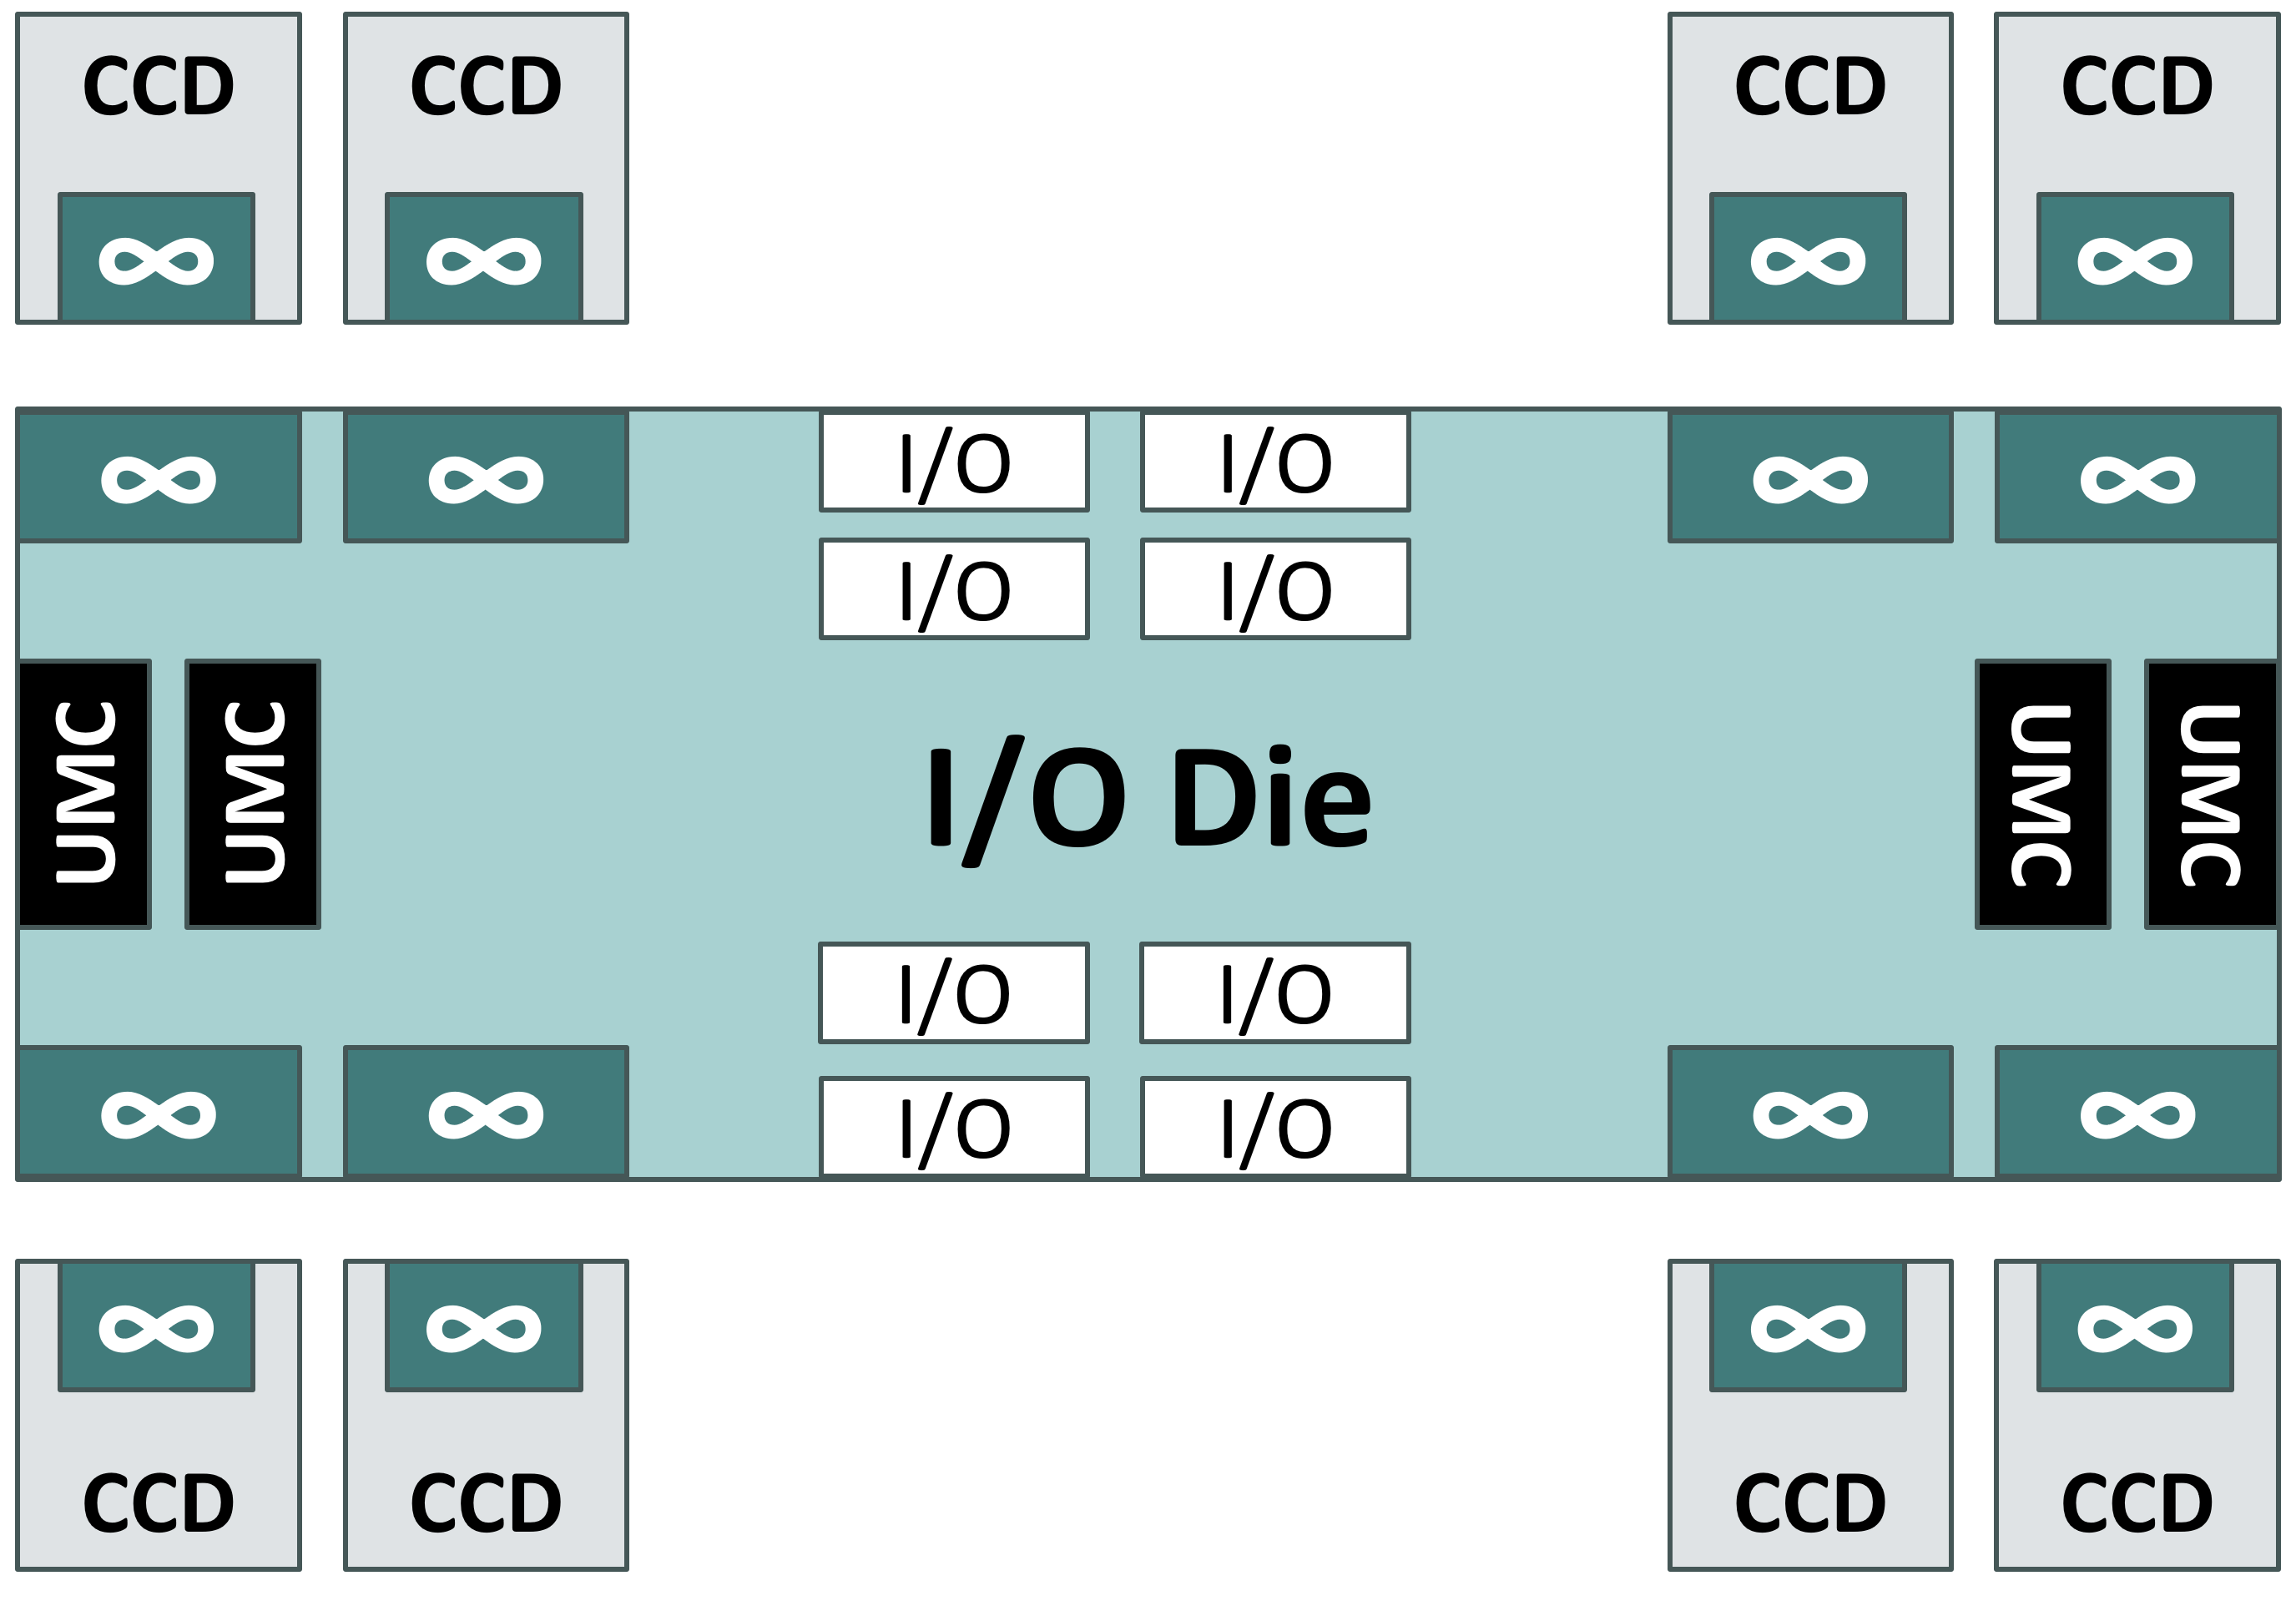
\includegraphics[width=\columnwidth]{figures/background/amd_arch/processor.png}
    \caption{AMD EPYC Zen 3 Architecture - CPU}
    \label{fig:amd-cpu}
\end{figure}


\Cref{fig:amd-cpu} shows a high-level overview of the architecture of the AMD EPYC Zen 3 processors.
The figure shows the following components:
\textbf{1) I/O:} The component that handles the input-output from the peripheral devices. This is where the PCIe communication happens.
\textbf{2) UMC:} The Unified Memory Controller is the controller that communicates with the DRAM.
\textbf{3) CCD:} The Core Complex Dies are where the cores (execution units) and caches reside.
\textbf{4) Infinity Fabric ($\infty$):} The interconnect that connects all of the components within the AMD CPU.

\subsubsection{CPU Pipelines}
\label{subsubsec:cpu-pipelines-bg}

Modern CPUs rely on executing multiple instructions simultaneously to maximise performance.
To achieve this, the CPUs have a multi-stage pipeline with the following stages: 1) Fetch, 2) Decode, 3) Schedule and Execute and 4) Retire.
We provide a simplified view of the pipeline in the CPU cores of the AMD EPYC Zen 3 processors in \Cref{fig:amd-core} and a brief description of each of the stages below:\\
\textbf{Fetch: } This stage fetches the next macro-op from the cache or the memory. 
However, the next macro-op to be fetched may not be deterministic, given the program may contain branches. 
In such cases, this stage also uses branch prediction to speculate on which instruction may be executed next and fetch that instruction.\\
\textbf{Decode: } This stage involved decoding the fetched macro-op into one or more micro-ops, which are then forwarded to the next stages.\\
\textbf{Schedule and Execute: } The scheduler(s) determine which instruction can be executed next based on the availability of the data that the instruction requires. 
This ensures that a long-running instruction (e.g., where the data is unavailable) does not stall all other independent instructions that can be executed.
As such, instructions here can be executed out of program order. 
Once the instruction has finished execution and the output of the instruction (if any) is available in the registers, the instruction is removed from the scheduler. 
\footnote{On AMD Zen 3 architecture, each scheduler has a capacity of 24 entries.}
As load and store are common but time-consuming instructions, this stage also consists of a load-store queue where pending load and store operations are held. \\
\textbf{Retire: } This stage ensures that instructions are retired in the program order so that the program can remain oblivious to the out-of-order execution that occurred in the previous stage.

\begin{figure}[!htb]
    \centering
    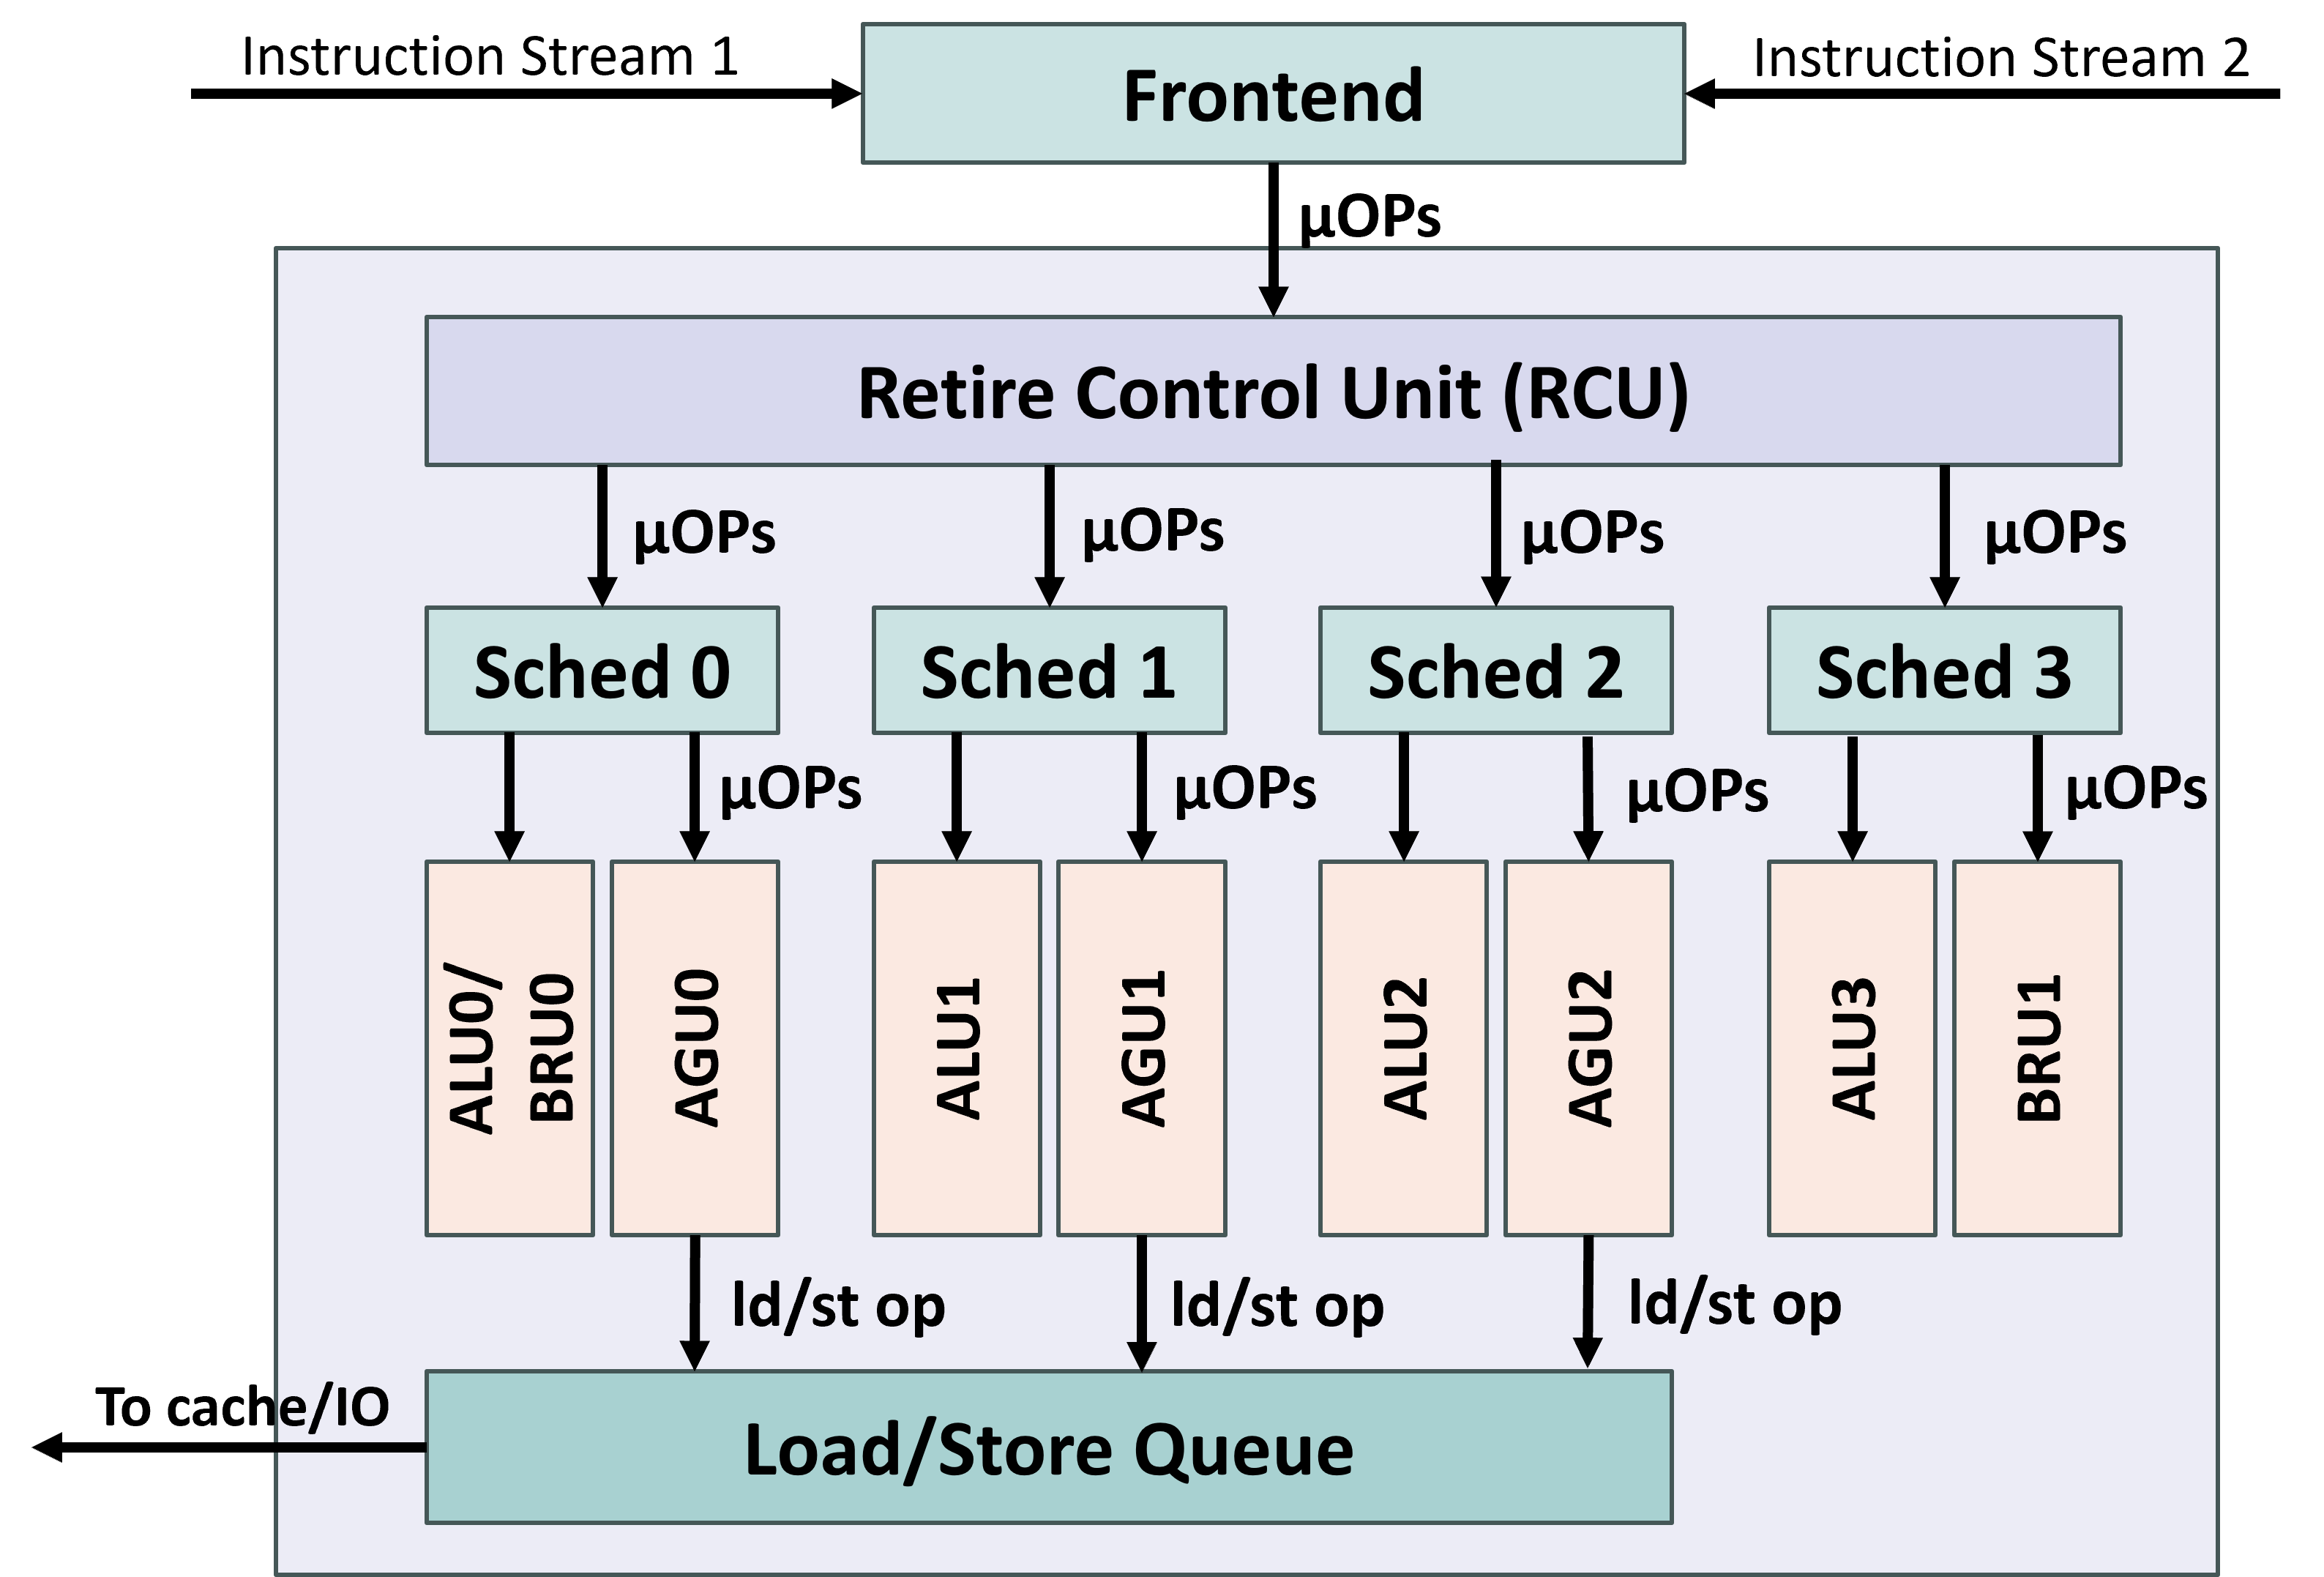
\includegraphics[width=\columnwidth]{figures/background/amd_arch/core.png}
    \caption{AMD EPYC Zen 3 Architecture - Core}
    \label{fig:amd-core}
\end{figure}

\subsubsection{PCIe transactions to/from CPU}

A program running on the CPU can transfer data to the PCIe device/endpoint in two major ways: 1) Memory operations via memory-mapped IO (MMIO) and 2) Direct memory access (DMA).
MMIO enables the CPU to map some memory region of the PCIe endpoint in the CPU's physical address space.
Any process with the proper permissions can then map this memory within the process and perform normal \textit{load} or \textit{store} operations on this memory.
However, this approach requires the execution units of the CPU to issue repeated \textit{load/store} instructions to copy data to the PCIe endpoint.
While this method is useful for reading or writing limited content, such as small configuration parameters, to the PCIe endpoints, it is inefficient for transferring a large amount of data.
To alleviate this, a lot of PCIe endpoints consist of a special hardware component called a DMA engine.
The DMA engine can copy large chunks of contiguous data without involving the execution units of the CPU.

For MMIO-based transactions, the load or store instructions go through the same instruction pipeline outlined in \Cref{fig:amd-core}. 
From the Load Store Queue, they end up in the I/O die outlined in \Cref{fig:amd-cpu} and go out the I/O block to the connected PCIe endpoint.
For DMA transactions (usually initiated by the PCIe endpoint), the transaction comes into the I/O block and, after some address and protocol translations, is sent out to the DRAM via the UMC.

\endinput


% \subsection{Threat Model}\label{subsec:interconnect-sc-threat-model}

\endinput
\chapter{NetShaper: A Differentially-Private Side Channel Mitigation System}

NetShaper \cite{sabzi2024netshaper} is both the name of the framework and the system that implements the framework to mitigate network side-channel attacks in internet applications.
We have provided a brief outline of the framework in \Cref{sec:netshaper-framework-bg}. 
Here, we describe the NetShaper system.

We first outline the requirements that the system should fulfil.
First, in any given window $W$, the system should be able to obtain the size of the payload in the buffering queue, with noise added to it. 
That is, the system should be able to complete the execution of $f_{DP}(S, t_{start}, t_{start} + W)$.
In the same window, the system should also be able to send out the payload, with padding, if necessary, such that the total data sent out, $b_{out}$, is equal to the noised size. 
However, it is sufficient to be able to queue $b_{out}$ bytes to be sent out, even if the actual transmission goes beyond the window $W$, as long as any delays were not caused by the payload coming in or already present in the buffering queue. 
The reason for this is the post-processing property of DP that we outlined in \Cref{subsec:dp-bg}.

Second, the payload and the padding should be indistinguishable to any observer observing the outbound packet stream.
Hence, the payload and padding should both be subject to the same congestion control, re-transmission, loss recovery, and other network behaviour.
In addition, the outbound transmission should provide the same or a higher level of reliability than the applications using this system expect.

Finally, the system should be modular so that modifications to any one sub-component do not require changes in the other components.
The system should also be portable and easily deployable, requiring none to minimal changes on the end hosts where the applications are running.
These goals ascertain that the system is easy to adopt and deploy and can easily be modified per the deployer's requirements.


% 1. Complete DP measurement within the window W
% 2. Data and Dummy should be indistinguishable
% 3. Should provide the same level of reliability the application expects
% 4. Should be modular for easy modification to sub-components
% 5. Should be portable and easily deployable, with minimal modifications of the end-hosts.

\section{Proxy Architecture}
\label{sec:proxy-arch}

\begin{figure}[!htb]
    \centering
    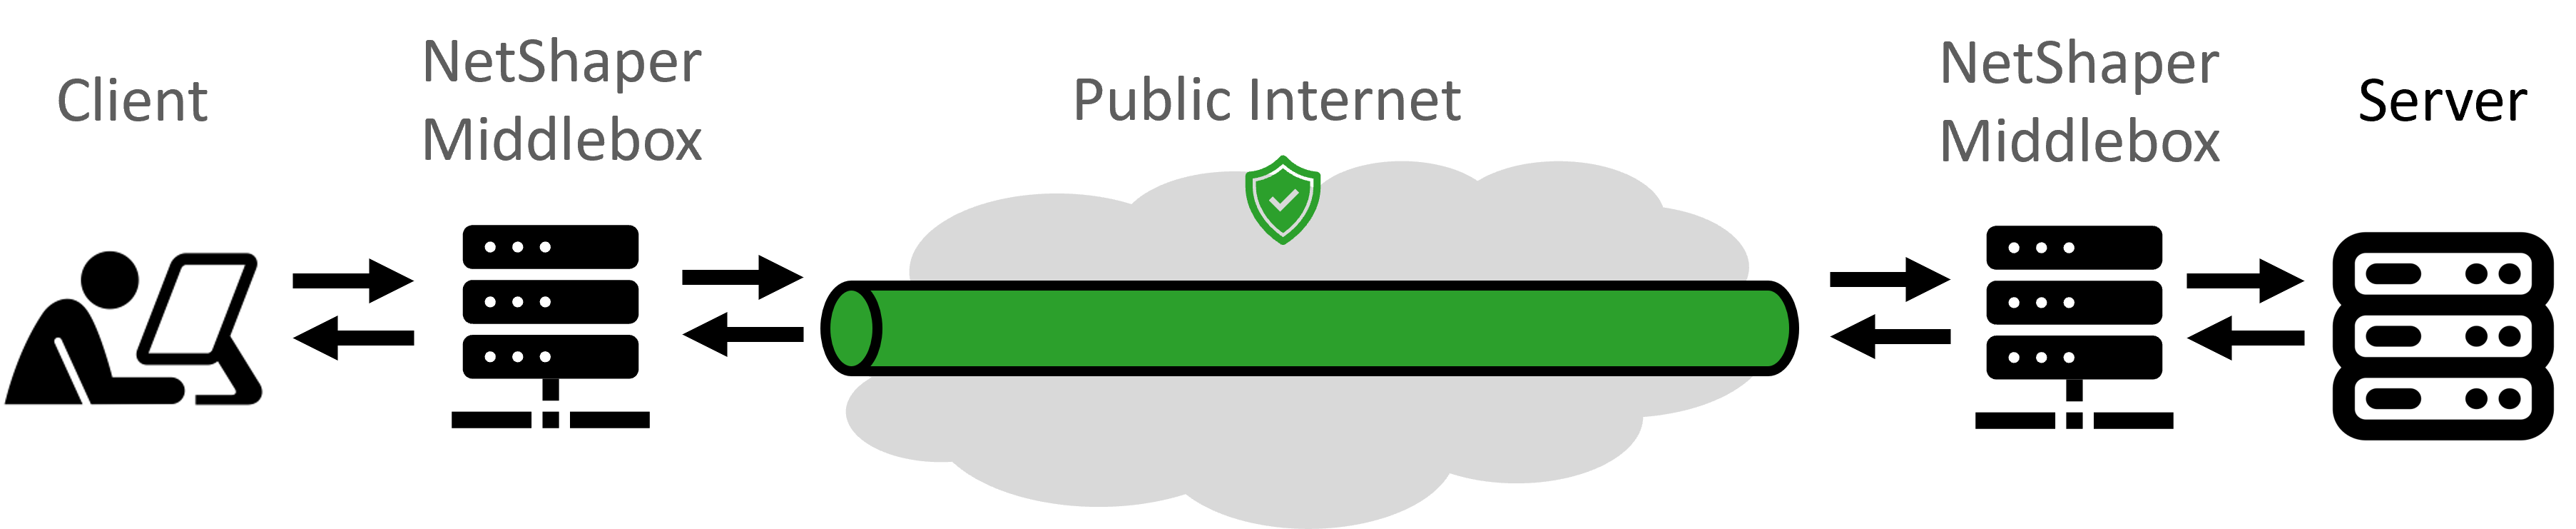
\includegraphics[width=\columnwidth]{figures/netshaper/netshaper-setup.png}
    \caption{NetShaper's Tunnel Setup}
    \label{fig:netshaper-setup}
\end{figure}

We designed NetShaper as a modular system that can be deployed using a pair of middleboxes, forming a forward and reverse proxy pair (see \Cref{fig:netshaper-setup}). 
Here, we describe in detail the architecture of the proxy setup and defer the discussion regarding the design of the middlebox to \Cref{sec:mb-design}. 

When using NetShaper, all clients communicate with the servers using three piecewise connections: 
(\textit{i}) between the client and the client-side middlebox, 
(\textit{ii}) between the client-side middlebox and the server-side middlebox, and
(\textit{iii}) between the server-side middlebox and the server.

For connection \textit{i} and \textit{iii}, NetShaper relies on standard TCP/UDP protocols. However, for connection \textit{ii} (i.e. to proxy the payload), NetShaper utilises QUIC. 
Using QUIC to proxy the payload avoids the TCP meltdown problem [??] that occurs when tunnelling TCP via TCP.
In addition, using QUIC also avoids the problem of an observer/attacker being able to distinguish between payload and padding that would occur when TCP was tunnelled via UDP (as the end host would retransmit payload, but the padding would not be retransmitted).

\paragraph{Setup.}
In order to be able to proxy end host traffic via NetShaper, the middleboxes need to be configured. 
The middleboxes first establish an encrypted QUIC connection between them, with user-specified reliability semantics.
Once the QUIC connection is established, NetShaper initialises three types of QUIC streams: Control, Data (Payload), and Dummy (Padding).
One \textit{control} stream is used to transmit messages regarding connection establishment or termination by the end host.
One \textit{dummy} stream is used for adding padding to the payload whenever necessary, based on the output of $f_{DP}$
\footnote{We avoid the use of PADDING frames in QUIC as they do not elicit acknowledgements and hence are distinguishable from the payload \cite{quic_rfc}.}.

\paragraph{Supporting multiple end hosts.}
As we discussed in \Cref{sec:quic-bg}, QUIC supports multiple streams in the same connection.
Using this, NetShaper can proxy the payload of multiple end hosts through a single QUIC connection between a pair of middleboxes.

While QUIC can support arbitrary initialisation and termination of streams, each stream has an associated header, which would increase the total transmission size.
For example, when transmitting two bytes in a single stream, the total transmission size would be $2 + S_{header}$.
However, when transmitting two streams of one byte each, the total transmission size would be $2 + 2*S_{header}$. 
An adversary may be able to distinguish between these two scenarios.
In order to avoid such a situation, NetShaper fixes and initialises a fixed number of streams per QUIC connection during the setup phase.
NetShaper assigns an unused stream to the client whenever a new client connects to the middlebox.
Similarly, NetShaper marks a stream as unused when an end host terminates the connection.

\endinput
\section{Middlebox Design}
\label{sec:mb-design}

While it is possible to apply NetShaper framework's approach at any network layer, we chose to develop the system as an L4 (Transport Layer) proxy.
This enables the system to be easily deployable, entirely in userspace and without requiring any superuser privileges. 
Developing NetShaper at L2 (Data Link Layer) or L3 (Network Layer) would require the deployer to either have the ability to modify the OS kernel or deploy some form of kernel bypass.

\begin{figure}[!htb]
    \centering
    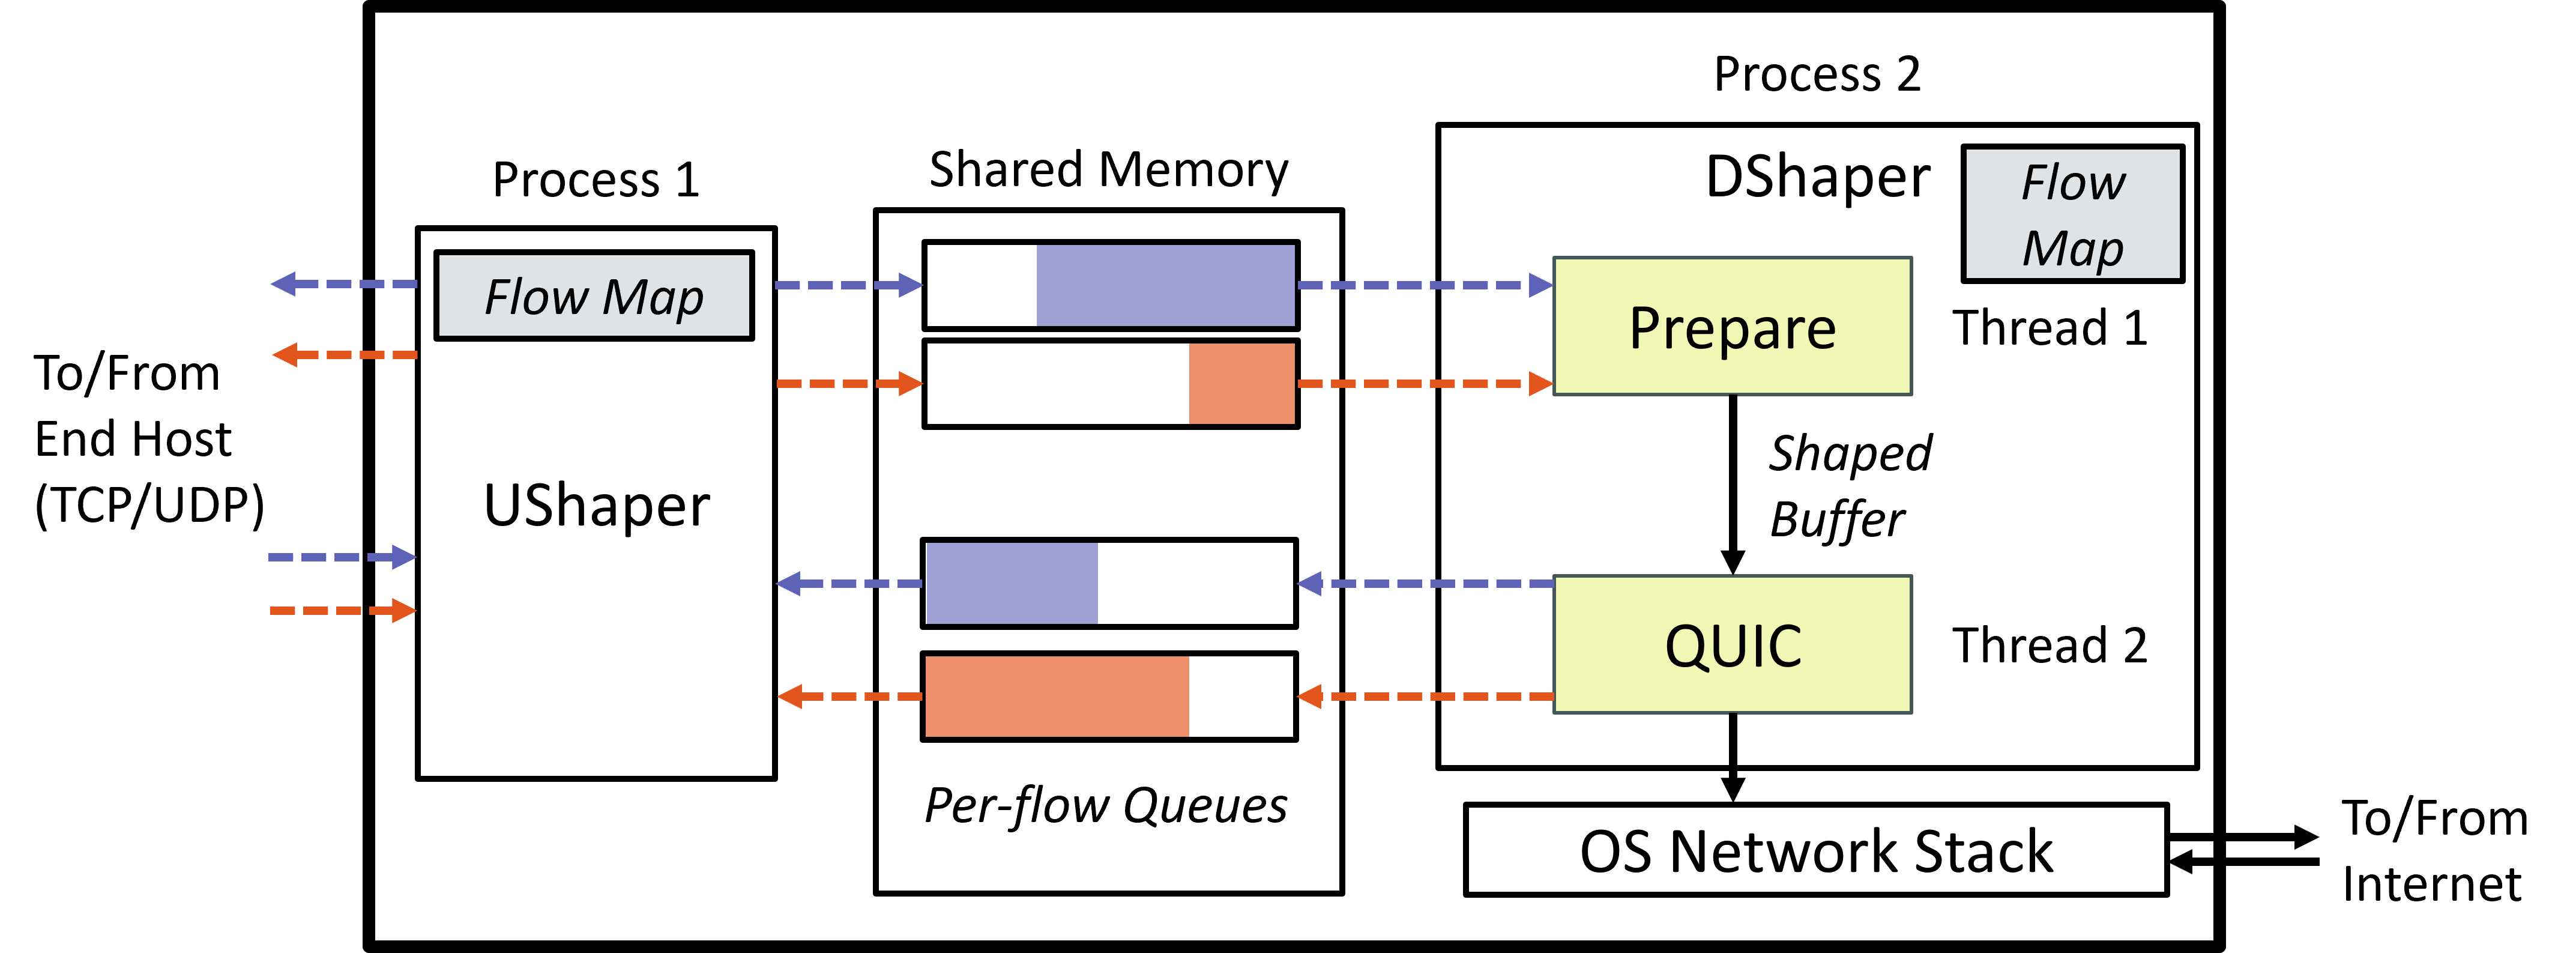
\includegraphics[width=\columnwidth]{figures/netshaper/middlebox-design.png}
    \caption{NetShaper Middlebox Design}
    \label{fig:middlebox-design}
\end{figure}

As outlined in \Cref{fig:middlebox-design}, NetShaper's middlebox consists of two main processes: UShaper and DShaper, and a shared memory between them.

\paragraph{UShaper.}
The \textit{UShaper} implements a client or a server to communicate with the end host.
It shares some Lamport Queues (LQs) [??] with DShaper.
It also consists of a flow map that maps a client with a corresponding pair of LQs.
\textit{UShaper} updates the flow map whenever a client establishes or terminates a connection.
In addition, it assigns an unused pair of LQs (one outbound and one inbound) to a new client and revokes that whenever the client terminates the connection.
The \textit{UShaper} receives outbound traffic from the end host and enqueues the payload in the assigned LQ.
Similarly, it dequeues inbound traffic from the inbound LQs and sends it to the corresponding end hosts.

\paragraph{DShaper.}
The \textit{DShaper} consists of two threads: \textit{Prepare} and \textit{QUIC worker}, and a flow map.
The flow map maps an LQ with a pre-initialised QUIC stream.
The \textit{Prepare} thread also measures the data available in the outbound LQs at the start of the window $W$.
It then adds noise to this available size based on the DP parameters.
Finally, it enqueues the payload and padding that needs to be transmitted.
The \textit{QUIC worker} transmits the enqueued data out to the network.
It also processes the received data, places it in the relevant LQ, and updates the flow map whenever a client initialises or terminates a connection.

In order to ensure that the operation of \textit{UShaper}, \textit{Prepare}, and \textit{QUIC worker} do not interfere with each other, we apply a few constraints in the implementation, and during the deployment of NetShaper.
First, all three components are required to be pinned on separate cores so that the execution time of one may not impact the others.
Second, in order to not leak the size of the payload due to the processing time of the enqueue operation done by the \textit{Prepare} thread, the \textit{Prepare} thread applies a lock for a fixed duration, during which the \textit{QUIC worker} can not transmit the data. 
We have outlined pseudo-code for both prepare and QUIC worker in \Cref{lst:prepare_and_worker}.
Finally, when receiving data, the \textit{QUIC worker} also enqueues the dummy bytes to a designated LQ so that the processing time remains consistent with the size of the data (see Figure ??).

\paragraph{Shared Memory.}
Both \textit{UShaper} and \textit{DShaper} have a shared memory between them.
This shared memory consists of three types of LQs: Control, Payload, Dummy
Similar to the stream types outlined in \Cref{sec:proxy-arch}, \textit{Control} LQ transmits the information about a connection establishment or termination by a client. 
\textit{Payload} LQ consists of the bytes received from the end host or to be sent to the end host.
\textit{Dummy} LQ consists of the dummy/padding bytes that are received.

\begin{minipage}{\textwidth}
\lstinputlisting[language=Python]{code/netshaper/prepare_and_worker.py}
\captionsetup{type=lstlisting}
\caption{Prepare and QUIC Worker Pseudo-code}
\label{lst:prepare_and_worker}
\end{minipage}

\endinput


\begin{figure}[!htb]
    \centering
    
\includegraphics[width=\columnwidth]{figures/netshaper/middlebox-design-overview.png}
    \caption{Overview of NetShaper's Middlebox}
    \label{fig:middlebox-design-overview}
\end{figure}

\endinput

Should we add pseudo-codes for UShaper and DShaper?
\section{Performance}\label{sec:netshaper-performance}
\section{Limitations and Discussion}\label{sec:netshaper-discussion}

\endinput
\chapter{Side Channel Attacks in Interconnects}

This chapter describes some avenues that can be used to carry out a side-channel attack on interconnects like PCIe and the challenges in pursuing those approaches.
In order to carry out a side-channel attack on PCIe, the first obvious step is to be able to transmit some data on the interconnect.
There are two major ways to achieve this: loads/stores on PCIe memory or configuration mapped to the CPU's address space or using DMA from the PCIe device to copy data to/from the CPU memory.
We describe the first approach in \Cref{sec:contention-with-stores}, and the second approach in \Cref{sec:contention-with-cudamemcpy}.


\section{Creating contention with load/store instructions}
\label{sec:contention-with-stores}

We have outlined the types of transactions PCIe supports in \Cref{tab:pcie-transaction-types}.
Most PCIe transactions are non-posted and, hence, are synchronous.
The synchronous behaviour enforces that no two load/store (i.e. read or write) operations to the same PCIe region can be issued in parallel.
However, having multiple parallel transactions that are in flight at the same time is necessary for the attacker to always have one pending packet in the PCIe buffer targeted for the side-channel attack
\footnote{An attacker can measure the delay in the transmission of that packet and infer the presence or absence of the victim traffic}.
As such, the attacker can only rely on non-posted transactions, and in particular, memory write operations
\footnote{While messages are also non-posted, they are usually generated by the underlying hardware directly, and the user has no control over those messages}.

In order to generate memory writes from the CPU, the attacker can map the device memory of a PCIe device, like a GPU, to an application running on the CPU and then issue store operations on that mapped memory.
Multiple store operations can be asynchronously issued on most modern processors as they support out-of-order execution. 
However, the same out-of-order execution feature makes it difficult for the attacker to accurately measure a store operation's time since the timer instruction can also be executed out of order.
In order to measure time accurately, most applications rely on issuing a fence instruction
\footnote{A fence instruction imposes ordering constraints, thus ensuring that any instruction after the fence is not executed before \textit{all} instructions before the fence are executed}.
However, this solution would not work for the attacker as the fence would not allow the next store instruction to be issued in parallel to the previous one, negating the benefit of using a posted (async) transaction.


\subsection{Measuring time of async stores}
\label{subsec:async_store_time}

In order to measure the completion time of a store operation which is issued out-of-order, we make use of two key insights:

\textit{First}, the CPU core would need to keep track of all instructions executed out-of-order so that they are retired in program order.
Keeping this track would require a scheduler and a buffer in the hardware, which would have a limited and fixed size.
The AMD CPU has four schedulers as described in \Cref{subsubsec:cpu-pipelines-bg}. Each scheduler has a fixed number of instruction slots $size_{sched}$.
In addition, for tracking load and store operations that are in flight, the CPU also has an LSQ, with a fixed number of slots for loads ($size_{ldq}$) and for stores ($size_{stq}$).
So, if the total number of pending (in flight) store instructions is larger than the total size of the scheduler slots and the store queue, the next instruction will be blocked, until one (or more) of the previous instructions finishes.

\textit{Second}, it is sufficient for the attacker to know if \textit{a} store instruction was delayed, and not if a particular store instruction was delayed.
% Convince why this is the case.
This would mean that we can use the first insight to queue a timer instruction immediately after issuing $size_{sched} + size_{stq}$ stores, and that timer will execute only after a store has completed.


\subsection{Evaluation}
\label{subsec:store-eval}

\endinput

\section{Creating contention with cudaMemcpy}
\label{sec:contention-with-cudamemcpy}

\section{Discussion}\label{sec:interconnect-sc-discussion}

\endinput

Should we consider the pre-microcode-update results and talk about that? It is NOT a vulnerability, just a behavioural observation. Hence, I don't think we need responsible disclosure
\chapter{Conclusion}

\section{Summary of Results}\label{sec:result-summary}
\section{Future Work}\label{sec:future-work}

\endinput


\begin{singlespace}
\raggedright
\bibliographystyle{abbrvnat}
\bibliography{biblio}
\end{singlespace}

\appendix
%    6. Appendices (including copies of all required UBC Research
%       Ethics Board's Certificates of Approval)
%\include{reb-coa}	% pdfpages is useful here
\chapter{Some Appendix}

\backmatter
%    7. Index
% See the makeindex package: the following page provides a quick overview
% <http://www.image.ufl.edu/help/latex/latex_indexes.shtml>


\end{document}


% Use this to generate only one chapter
% % To be used for generating only 1 chapter of the thesis

\title{Side-Channel Security in Networks: From the Internet to Interconnects}

\author{Rut Vora}
\previousdegree{B. Engineering in Computer Science, BITS-Pilani, 2020}


\degreetitle{Master of Science}

\institution{The University of British Columbia}
\campus{Vancouver}

\faculty{The Faculty of Graduate and Postdoctoral Studies}
\department{Computer Science}
\submissionmonth{March}
\submissionyear{2025}

\examiningcommittee{Aastha Mehta, Assistant Professor, Computer Science, \textsc{UBC}}{Supervisor}
% \examiningcommittee{Mathias L\'{e}cuyer, Assistant Professor, Computer Science, \textsc{UBC}}{Co-Supervisor}
% \examiningcommittee{Margo Seltzer, Professor, Computer Science, \textsc{UBC}}{Supervisory Committee Member}

%% hyperref package provides support for embedding meta-data in .PDF
%% files
\hypersetup{
  pdftitle={Side-Channel Security in Networks: From the Internet to Interconnects  (DRAFT: \today)},
  pdfauthor={Rut Vora},
  pdfkeywords={PCIe, CXL, Side Channels, Networks, Proxy}
}

\begin{document}

\maketitle

\textspacing		% begin one-half or double spacing

% Body of Thesis (not all sections may apply)
\mainmatter

\acresetall	% reset all acronyms used so far

% Main Sections
% \chapter{Background}

% We begin this chapter by discussing the problem of network side-channel attacks in \Cref{sec:ns-attacks}, in the context of two distinct applications: video streaming and web services.
% In \Cref{sec:dp-background}, we present a comprehensive definition of differential privacy (DP), outline its key properties, and highlight its primary applications, thereby setting the foundation for our differentially private traffic shaping mechanism.
% In \Cref{sec:background-quic} we provide a brief overview of the QUIC protocol, which plays a pivotal role in the design of {\sys}.
% Finally, in \Cref{sec:threat-model}, we conclude this chapter by explaining our threat model. 

\section{Network Side Channels}
\label{sec:network-side-channel-background}

Let us first understand how network side-channel attacks are carried out.
The ultimate goal of the attacker is to determine the contents of the web traffic being transmitted or received by the victim. More often than not, an attacker is interested in knowing if the victim accessed any content from a small subset and, if so, which content they accessed.
To do this, the attacker takes the following steps: 
1) Collect network traces
2) Build a classifier trained on the collected network traces
3) Gain access to the network shared with the victim
4) Profile the victim's network traffic
5) Determine whether the victim accessed any content of interest to the attacker

First, the attacker builds a collection of the content (e.g. webpages and video streams) that they are interested in. 
They collect network traces for this content under various network conditions to account for variability caused by the network itself. 
Then, the attacker trains a classifier on this collected network trace.
The classifier can use multiple features like packer sizes, inter-packer timing, total bytes transferred in a burst of packets, the duration of the burst and the interval between bursts, and the direction of the bursts \cite{schuster2017beautyburst}.

Next, the attacker infiltrates a machine that shares some network path with the victim.
This machine could also be the victim's machine. 
The malicious application could be a javascript-based advertisement on the page the victim is visiting or another process on the victim's machine, thus sharing the network card on that machine. 
It could also be a shared router/switch in the victim's network path to the server.
The attacker could either be another client connected to the same shared router/switch or someone who owns the router/switch.
If the attacker owns an element in the network path, they can directly observe all the features necessary to carry out the attack. 
Otherwise, they create congestion in the shared network path such that the victim's network traffic would contend with the attacker's traffic.
In this case, the attacker's traffic would be delayed, and the delay would be proportional to the victim's traffic, thus revealing some features of the victim's traffic.

The attacker collects the network traces of its own traffic and, based on that, extracts the features of the victim's traffic flow. These extracted features are then run through the pre-trained classifier, which helps the attacker determine which content the victim accessed. \citeauthor{schuster2017beautyburst} demonstrated that one could train a Convolution Neural Network (CNN)-based classifier to determine which video the victim is streaming. Similarly, prior work has demonstrated that such a network side channel-based approach can also be used to determine which webpage the victim is visiting \cite{hayes2016kfp, panchenko2016website, gong2010fingerprinting}

% \section{Threat Model}\label{sec:nsc-threat-model}

\section{NetShaper - Framework}
\label{sec:netshaper-framework-bg}

NetShaper \cite{sabzi2024netshaper} is both the name of a differential-privacy-based framework for mitigating network side-channel attacks and the system that utilises that framework. 
Here, we provide a brief description of the NetShaper Framework.

\subsection{Differential Privacy}
NetShaper's framework relies on Differential Privacy (DP) to provide robust, mathematical guarantees against side-channel attacks in internet networks.
DP is a framework originally proposed by \citeauthor{dwork2006differential} for releasing usable aggregate metrics regarding a dataset while limiting the leakage of information about individual data points in that dataset.
In other words, DP bounds the probability of an observer being able to infer if an individual data point was used to generate the aggregate metric the observer has access to.
DP has two main parameters: \\
\textbf{$\epsilon$: } Intuitively, it specifies the amount of privacy loss
\textbf{$\delta$: } Intuitively, it specifies the probability with which a given differentially-private mechanism can fail.


\begin{definition}[Differential privacy]
  \label{def:dp}
  A randomized algorithm $A_{DP}$ is $(\varepsilon, \delta)-DP$ if for all ${S} \subseteq Range(A_{DP})$ and for all datasets $D, D'$ that differ on a single element, we have:
  \begin{equation*}
    \Pr[A_{DP}(D) \in S] \leq \exp(\varepsilon)\Pr[A{DP}(D') \in S] + \delta
  \end{equation*}
\end{definition}

For any aggregate algorithm $A$, we can make an $(\varepsilon, \delta)-DP$ algorithm by adding some noise to the output of $A$.
There are many different mechanisms to add the noise $\eta$, but most commonly, $\eta$ is a function of $\varepsilon, \delta$ and other dataset-dependent parameters. 
Mathematically, $A_{DP}(D) = A(D) + \eta(\varepsilon, \delta, ...)$

DP has a few useful properties: 
\textbf{1) Post Processing:} Any further operations or processing on the output of an $(\varepsilon, \delta)-DP$ algorithm is also $(\varepsilon, \delta)-DP$.
This condition holds true as long as the operations carried out do not involve any auxiliary knowledge of the dataset.
\textbf{2) Composition:} It is possible to quantify the total privacy loss when multiple queries are issued to the same $(\varepsilon, \delta)-DP$ algorithm.

\subsection{Applying DP on network streams}
NetShaper uses DP to mitigate network side-channel attacks. 
To achieve this, NetShaper relies on two key ideas: 
First, NetShaper represents network traffic streams as datasets to which DP can be applied.
As DP applies to datasets, we must first represent a network stream as a dataset.
A network stream $S$ can be represented as a sequence of packets $P_i^S$, where each packet is associated with its length and the timestamp at which it was encountered (i.e. $P_i^S = (l_i^S, t_i^S$).
Hence, $S$ is the dataset consisting of the traffic shape, which can be used by an attacker to carry out a side-channel attack, as outlined in \Cref{sec:network-side-channel-background}.
As the network stream can potentially be long, NetShaper models the DP guarantees in windows of fixed length $W$ and can use composition to calculate the privacy loss across multiple windows.
Second, NetShaper relies on a buffering queue to control the shape of the traffic visible to the attacker within each window $W$ by discretising time into $W$-sized windows.
At the beginning of each discrete window, NetShaper checks the size of the buffer and adds DP noise to the size to determine the amount of data to be sent out in that window.


So, initially, the attacker was able to query a function $f(S, t_{start}, t_{end})$ to obtain the size and time of the packet that was transmitted by the victim. 
However, with the application of DP on the network stream, the attacker can now only query a new function $f_{DP}(S, t_{start}, t_{end})$.
$f_{DP}$ is a differentially private function ensuring that the probability of leaking individual entries of the dataset is bounded, and where $t_{end} - t_{start} = kW, k \in N$.

\endinput

Note: Should we add stuff about sensitivity? (I don't think it's necessary for my thesis)
\section{The QUIC protocol}
\label{sec:quic-bg}

QUIC is a connection-oriented transport layer protocol that can be deployed on top of UDP.
It is now standardised under RFC 9000 \cite{quic_rfc}.
It provides many features which are similar to TCP, like flow control, loss recovery, and congestion control. 
However, it also alleviates some problems that TCP encounters.
For example, QUIC enforces encryption in the initial handshake, thus ensuring that all traffic is always encrypted.
In addition, a QUIC connection can consist of multiple dynamically created streams, each of which can act as an independent byte stream. 
This helps alleviate the problem of head-of-line blocking faced by TCP, ensuring that one blocked stream does not affect others.
Each stream has a unique header containing the stream ID and the stream type, among other information.
Multiple such streams, with their headers, can be a part of a single encrypted QUIC packet.
This ensures that an attacker can not determine the number of streams being transmitted in a QUIC packet just by observing the encrypted packet or traffic stream.


\endinput

\footnote{While QUIC has a PADDING frame, we don't use it, as a packet that only contains padding frames will not be re-transmitted in case of packet loss, thus revealing that it was a dummy packet.}


\section{Side Channels in Interconnects}
\label{sec:interconnect-sc-bg}
Conceptually, carrying out a side-channel interconnect is very similar to carrying out such an attack on internet networks. 
The attacker creates congestion on a buffer in the communication path between the host (CPU) and the peripheral (e.g. GPU) and observes their own delay.
This delay would be proportional to the amount of data transferred by the victim, which would help the attacker gain insight into the victim's traffic shape.

However, a few differences between interconnects and traditional networks make it challenging to implement such an attack. \\
\textit{First}, The bandwidth of interconnects like PCIe is at least an order of magnitude higher than that of internet networks.
While a typical bandwidth in an internet network may be 1-10Gbps ( = 0.125 - 1.25 GBps), PCIe 4.0 can operate at a rate of 32GBps.
The high bandwidth makes it non-trivial to saturate the PCIe link. \\
\textit{Second}, latency in PCIe is at least three orders of magnitude smaller than that of internet networks.
Typically, internet latency is measured in milliseconds, while PCIe latency is measured in microseconds.
The low latency makes it difficult for the attacker to measure the delays accurately. \\
\textit{Third}, unlike internet networks, PCIe does not extend outside the machine of the host CPU.
This further adds to the challenge that the attacker needs to co-locate with the victim application on the same machine. \\
\textit{Fourth}, the PCIe protocol has a fixed behaviour depending on the type of transaction. 
Most transaction types can not generate enough traffic to even come close to saturating the bandwidth of PCIe. 
While saturating the bandwidth may not be necessary to create a side-channel attack, it would be useful if there is always at least one attacker packet in the buffer whenever the victim might transmit.
This would ensure that the attacker can observe a delay in their own packets for each packet or set of packets the victim transmits.

We provide a list of the transactions PCIe supports in \Cref{tab:pcie-transaction-types}, and a description of what each PCIe transaction type entails below: \\
\textbf{Posted:} Transactions where no response is issued or expected. 
These transactions are also asynchronous and hence allow multiple transactions of the same type to be in flight at the same time.\\
\textbf{Non-posted:} Transactions where a response is required. 
These types of transactions are also synchronous.
As such, one can not execute multiple of these simultaneously.\\
\textbf{Completions:} The completion of a previous non-posted transaction.\\

\begin{table}[htb]
    \centering
    \begin{tabular}{|l|l|p{0.65\textwidth}|}
        \hline
        \textbf{Transaction} & \textbf{Type} & \textbf{Description} \\ 
        \hline
        Memory Read  & Non-Posted & Read from a memory-mapped address space \\ 
        Memory Write & Posted     & Write to a memory-mapped address space  \\ 
        I/O Read     & Non-Posted & (Legacy PCI) Read from the I/O address space \\ 
        I/O Write    & Non-Posted & (Legacy PCI) Write to the I/O address space \\ 
        Config Read  & Non-Posted & Read control and status registers of the PCIe interface \\ 
        Config Write & Non-Posted & Write control and status registers of the PCIe interface \\  
        Message      & Posted     & Conveys additional information (e.g. Interrupts, Power Management, Error Signalling, Vendor-defined messaging). \\
        Completion   & Completion & Response to all non-posted transactions \\ 
        \hline
    \end{tabular}
    \caption{PCIe transaction types}
    \label{tab:pcie-transaction-types}
\end{table}


\subsection{Challenge: Measuring the time of PCIe transactions}

In \Cref{tab:pcie-transaction-types}, we can see that most PCIe transactions are Non-posted.
Only memory writes and messages are posted and hence asynchronous.
Asynchronous transactions such as a memory write (i.e. a \textit{store} instruction executed on memory-mapped PCIe endpoint memory region) would be more useful for carrying out a side-channel attack on PCIe.
This is because asynchronous transactions enable the attacker to have one transaction always pending to be sent out, regardless of the completion of the previous transaction(s).

However, measuring the completion time of an individual asynchronous transaction becomes more challenging as they are executed out-of-order. 
The naive solution of having a memory fence after each \textit{store} instruction would not work, as the memory fence would not allow the next \textit{store} instruction to be issued in parallel to the previous one, negating the benefit of using an asynchronous transaction.

\endinput




https://www.linkedin.com/pulse/pci-express-primer-3-transaction-layer-simon-southwell/
\section{AMD CPU Architecture}
\label{subsec:amd-arch-bg}

Modern CPUs consist of many components, such as execution units, caches, PCIe root complex, and DRAM controllers.
Some subset of these components is always traversed when data is sent to or from the CPU to the PCIe endpoints.
The behaviour of each individual component may impact how the side-channel attack is carried out.
As such, it becomes necessary to understand all the components that may be involved in a PCIe transaction.

\begin{figure}[!htb]
    \centering
    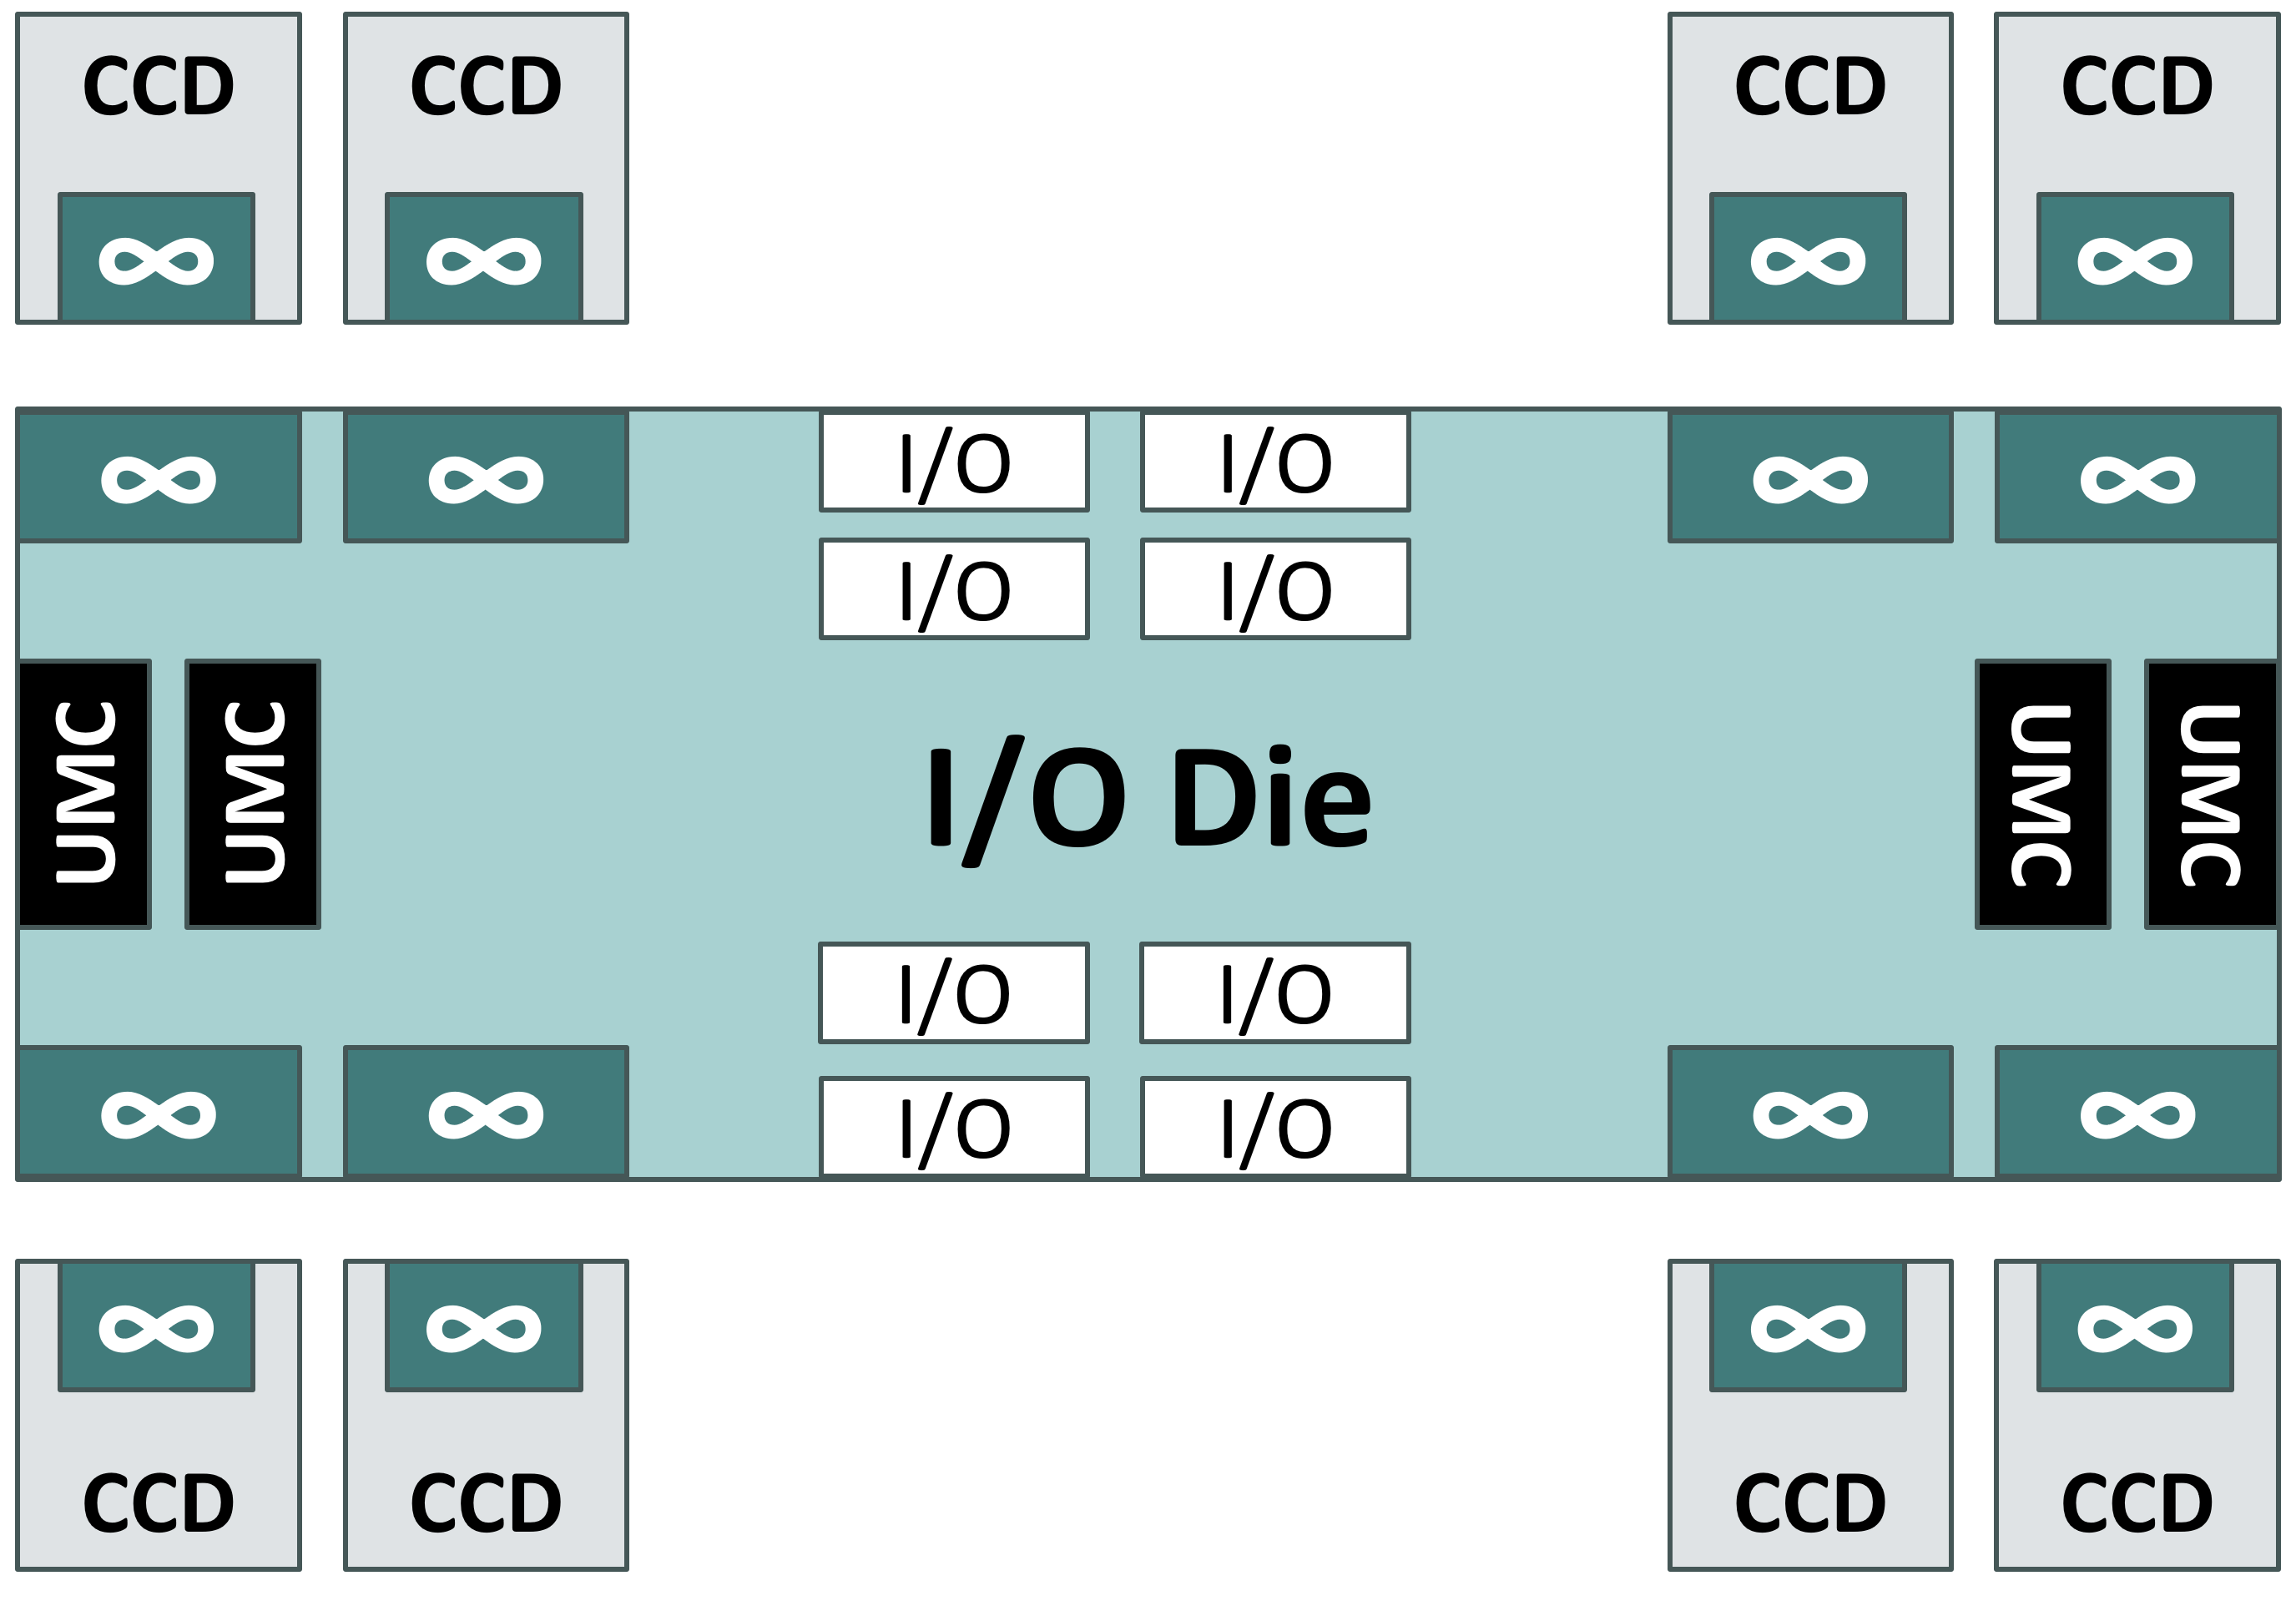
\includegraphics[width=\columnwidth]{figures/background/amd_arch/processor.png}
    \caption{AMD EPYC Zen 3 Architecture - CPU}
    \label{fig:amd-cpu}
\end{figure}


\Cref{fig:amd-cpu} shows a high-level overview of the architecture of the AMD EPYC Zen 3 processors.
The figure shows the following components:
\textbf{1) I/O:} The component that handles the input-output from the peripheral devices. This is where the PCIe communication happens.
\textbf{2) UMC:} The Unified Memory Controller is the controller that communicates with the DRAM.
\textbf{3) CCD:} The Core Complex Dies are where the cores (execution units) and caches reside.
\textbf{4) Infinity Fabric ($\infty$):} The interconnect that connects all of the components within the AMD CPU.

\subsubsection{CPU Pipelines}
\label{subsubsec:cpu-pipelines-bg}

Modern CPUs rely on executing multiple instructions simultaneously to maximise performance.
To achieve this, the CPUs have a multi-stage pipeline with the following stages: 1) Fetch, 2) Decode, 3) Schedule and Execute and 4) Retire.
We provide a simplified view of the pipeline in the CPU cores of the AMD EPYC Zen 3 processors in \Cref{fig:amd-core} and a brief description of each of the stages below:\\
\textbf{Fetch: } This stage fetches the next macro-op from the cache or the memory. 
However, the next macro-op to be fetched may not be deterministic, given the program may contain branches. 
In such cases, this stage also uses branch prediction to speculate on which instruction may be executed next and fetch that instruction.\\
\textbf{Decode: } This stage involved decoding the fetched macro-op into one or more micro-ops, which are then forwarded to the next stages.\\
\textbf{Schedule and Execute: } The scheduler(s) determine which instruction can be executed next based on the availability of the data that the instruction requires. 
This ensures that a long-running instruction (e.g., where the data is unavailable) does not stall all other independent instructions that can be executed.
As such, instructions here can be executed out of program order. 
Once the instruction has finished execution and the output of the instruction (if any) is available in the registers, the instruction is removed from the scheduler. 
\footnote{On AMD Zen 3 architecture, each scheduler has a capacity of 24 entries.}
As load and store are common but time-consuming instructions, this stage also consists of a load-store queue where pending load and store operations are held. \\
\textbf{Retire: } This stage ensures that instructions are retired in the program order so that the program can remain oblivious to the out-of-order execution that occurred in the previous stage.

\begin{figure}[!htb]
    \centering
    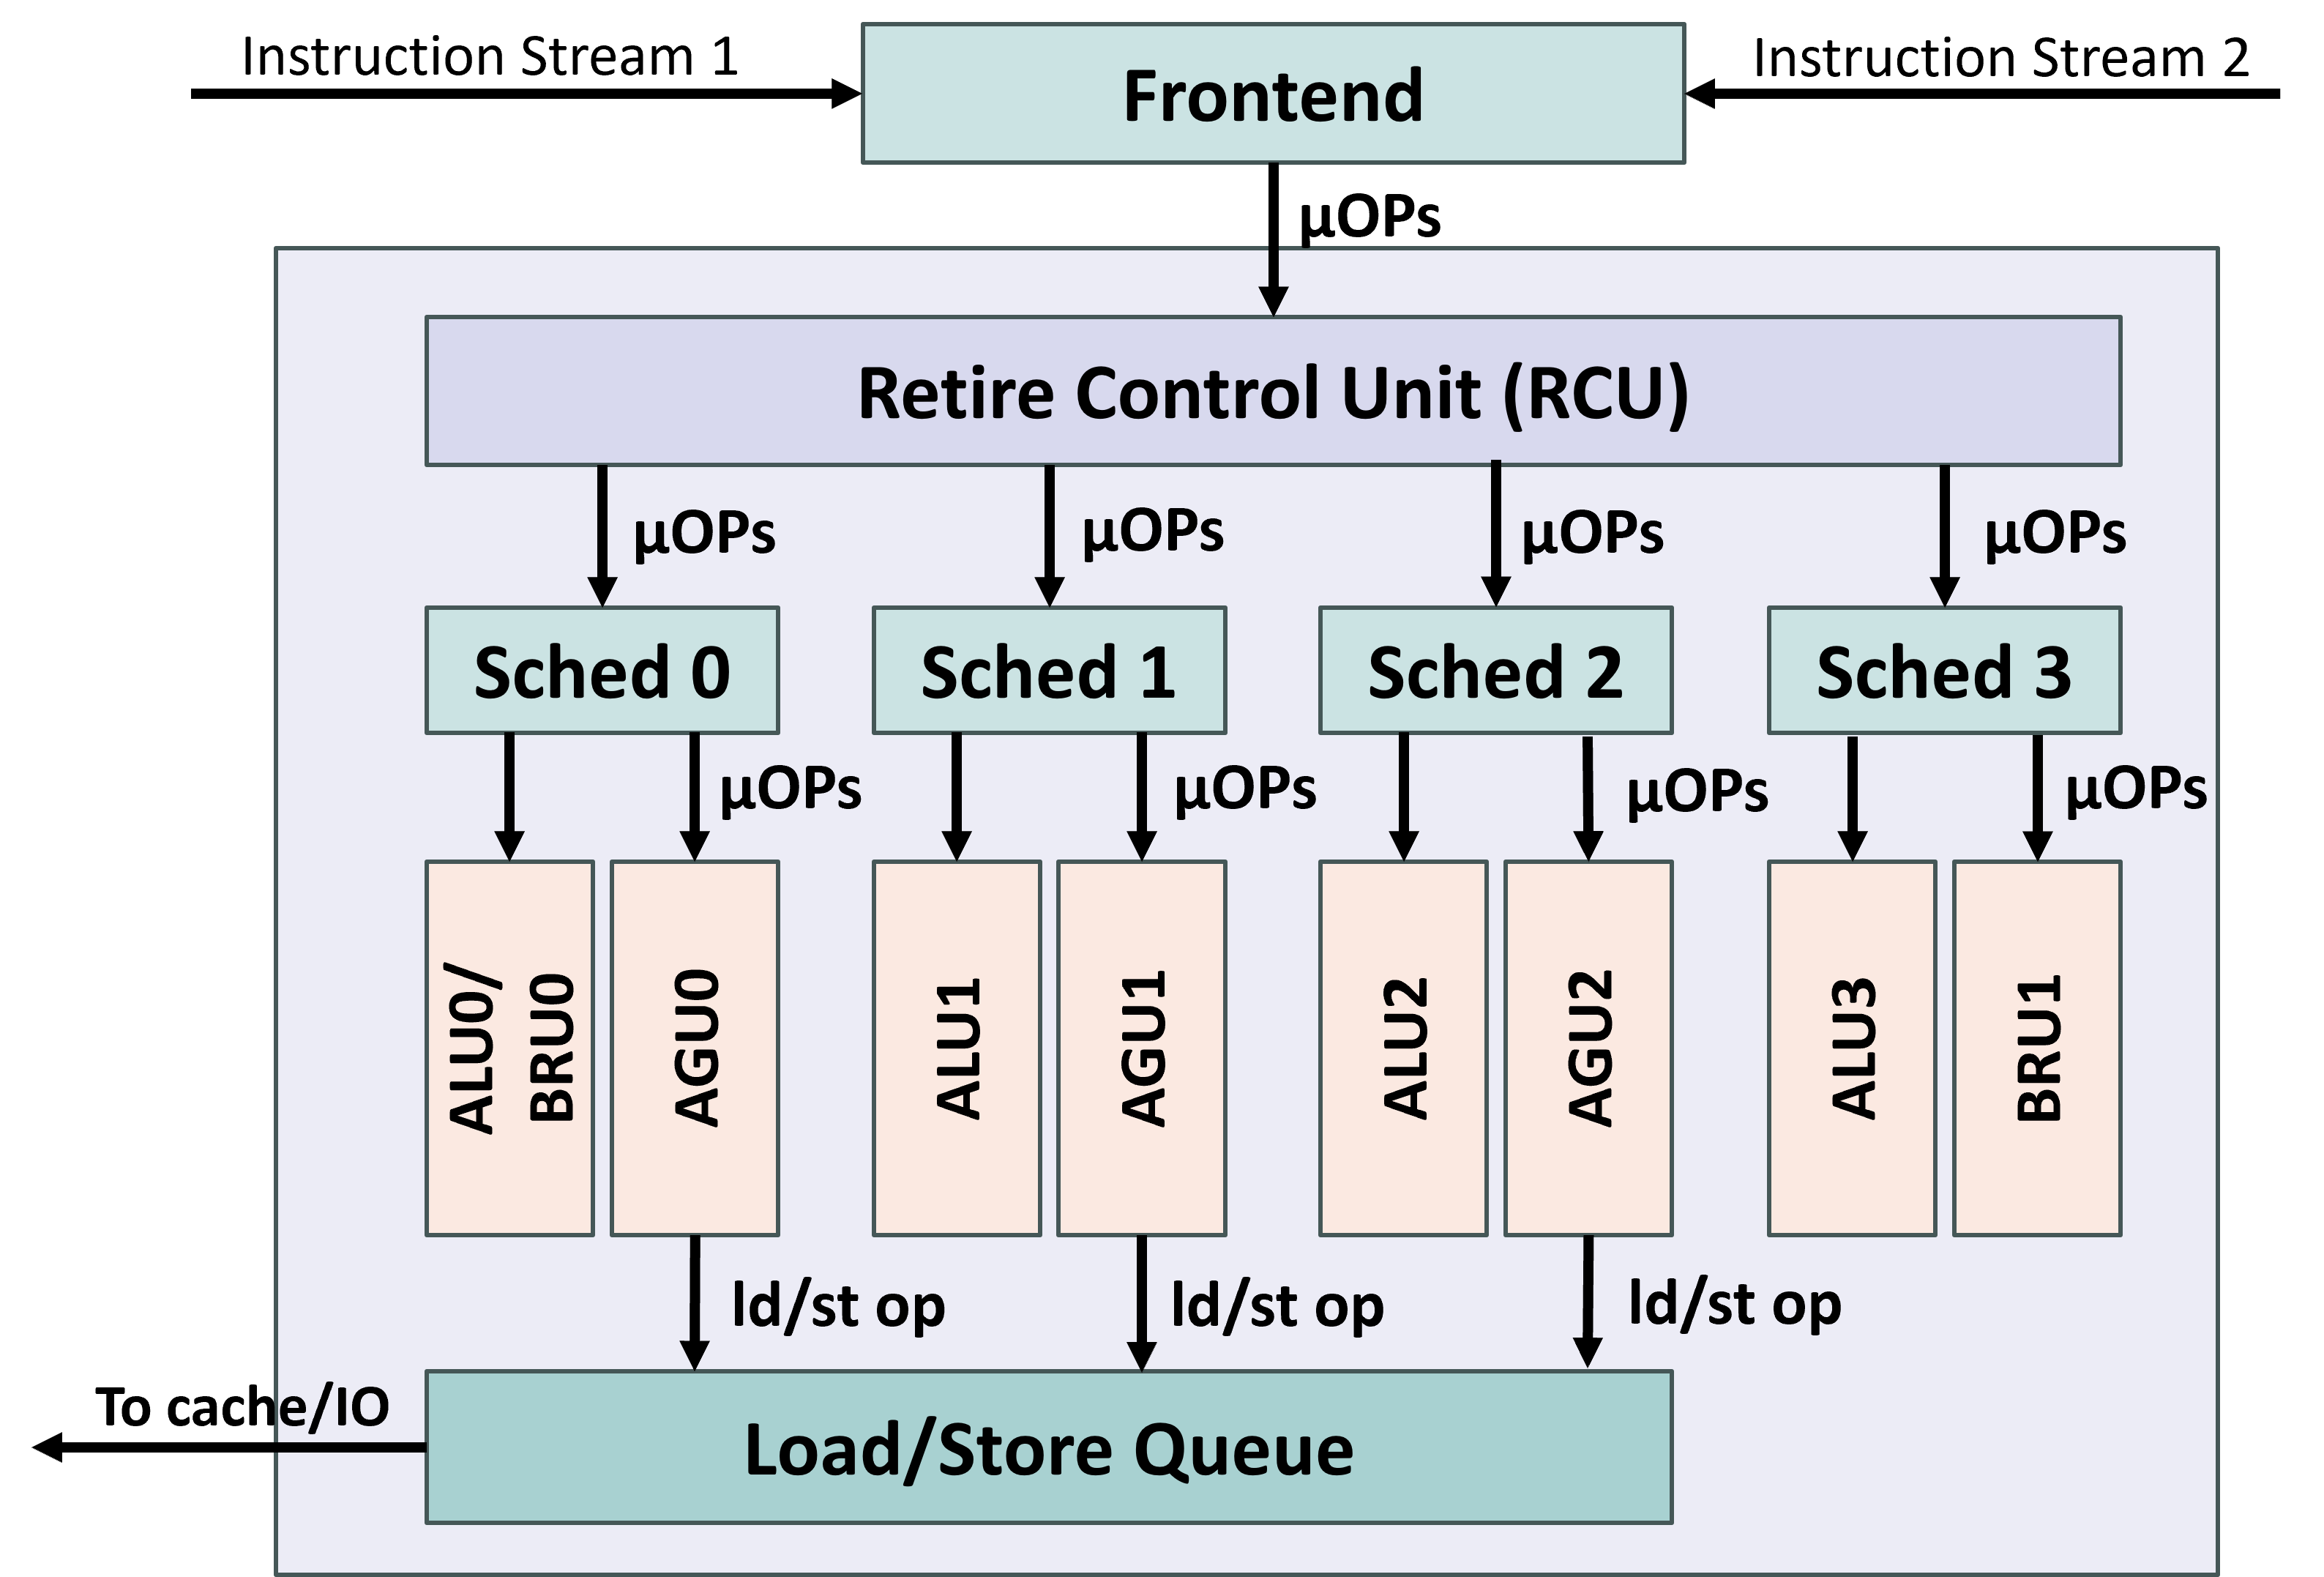
\includegraphics[width=\columnwidth]{figures/background/amd_arch/core.png}
    \caption{AMD EPYC Zen 3 Architecture - Core}
    \label{fig:amd-core}
\end{figure}

\subsubsection{PCIe transactions to/from CPU}

A program running on the CPU can transfer data to the PCIe device/endpoint in two major ways: 1) Memory operations via memory-mapped IO (MMIO) and 2) Direct memory access (DMA).
MMIO enables the CPU to map some memory region of the PCIe endpoint in the CPU's physical address space.
Any process with the proper permissions can then map this memory within the process and perform normal \textit{load} or \textit{store} operations on this memory.
However, this approach requires the execution units of the CPU to issue repeated \textit{load/store} instructions to copy data to the PCIe endpoint.
While this method is useful for reading or writing limited content, such as small configuration parameters, to the PCIe endpoints, it is inefficient for transferring a large amount of data.
To alleviate this, a lot of PCIe endpoints consist of a special hardware component called a DMA engine.
The DMA engine can copy large chunks of contiguous data without involving the execution units of the CPU.

For MMIO-based transactions, the load or store instructions go through the same instruction pipeline outlined in \Cref{fig:amd-core}. 
From the Load Store Queue, they end up in the I/O die outlined in \Cref{fig:amd-cpu} and go out the I/O block to the connected PCIe endpoint.
For DMA transactions (usually initiated by the PCIe endpoint), the transaction comes into the I/O block and, after some address and protocol translations, is sent out to the DRAM via the UMC.

\endinput


% \subsection{Threat Model}\label{subsec:interconnect-sc-threat-model}

\endinput
\chapter{NetShaper: A Differentially-Private Side Channel Mitigation System}

NetShaper \cite{sabzi2024netshaper} is both the name of the framework and the system that implements the framework to mitigate network side-channel attacks in internet applications.
We have provided a brief outline of the framework in \Cref{sec:netshaper-framework-bg}. 
Here, we describe the NetShaper system.

We first outline the requirements that the system should fulfil.
First, in any given window $W$, the system should be able to obtain the size of the payload in the buffering queue, with noise added to it. 
That is, the system should be able to complete the execution of $f_{DP}(S, t_{start}, t_{start} + W)$.
In the same window, the system should also be able to send out the payload, with padding, if necessary, such that the total data sent out, $b_{out}$, is equal to the noised size. 
However, it is sufficient to be able to queue $b_{out}$ bytes to be sent out, even if the actual transmission goes beyond the window $W$, as long as any delays were not caused by the payload coming in or already present in the buffering queue. 
The reason for this is the post-processing property of DP that we outlined in \Cref{subsec:dp-bg}.

Second, the payload and the padding should be indistinguishable to any observer observing the outbound packet stream.
Hence, the payload and padding should both be subject to the same congestion control, re-transmission, loss recovery, and other network behaviour.
In addition, the outbound transmission should provide the same or a higher level of reliability than the applications using this system expect.

Finally, the system should be modular so that modifications to any one sub-component do not require changes in the other components.
The system should also be portable and easily deployable, requiring none to minimal changes on the end hosts where the applications are running.
These goals ascertain that the system is easy to adopt and deploy and can easily be modified per the deployer's requirements.


% 1. Complete DP measurement within the window W
% 2. Data and Dummy should be indistinguishable
% 3. Should provide the same level of reliability the application expects
% 4. Should be modular for easy modification to sub-components
% 5. Should be portable and easily deployable, with minimal modifications of the end-hosts.

\section{Proxy Architecture}
\label{sec:proxy-arch}

\begin{figure}[!htb]
    \centering
    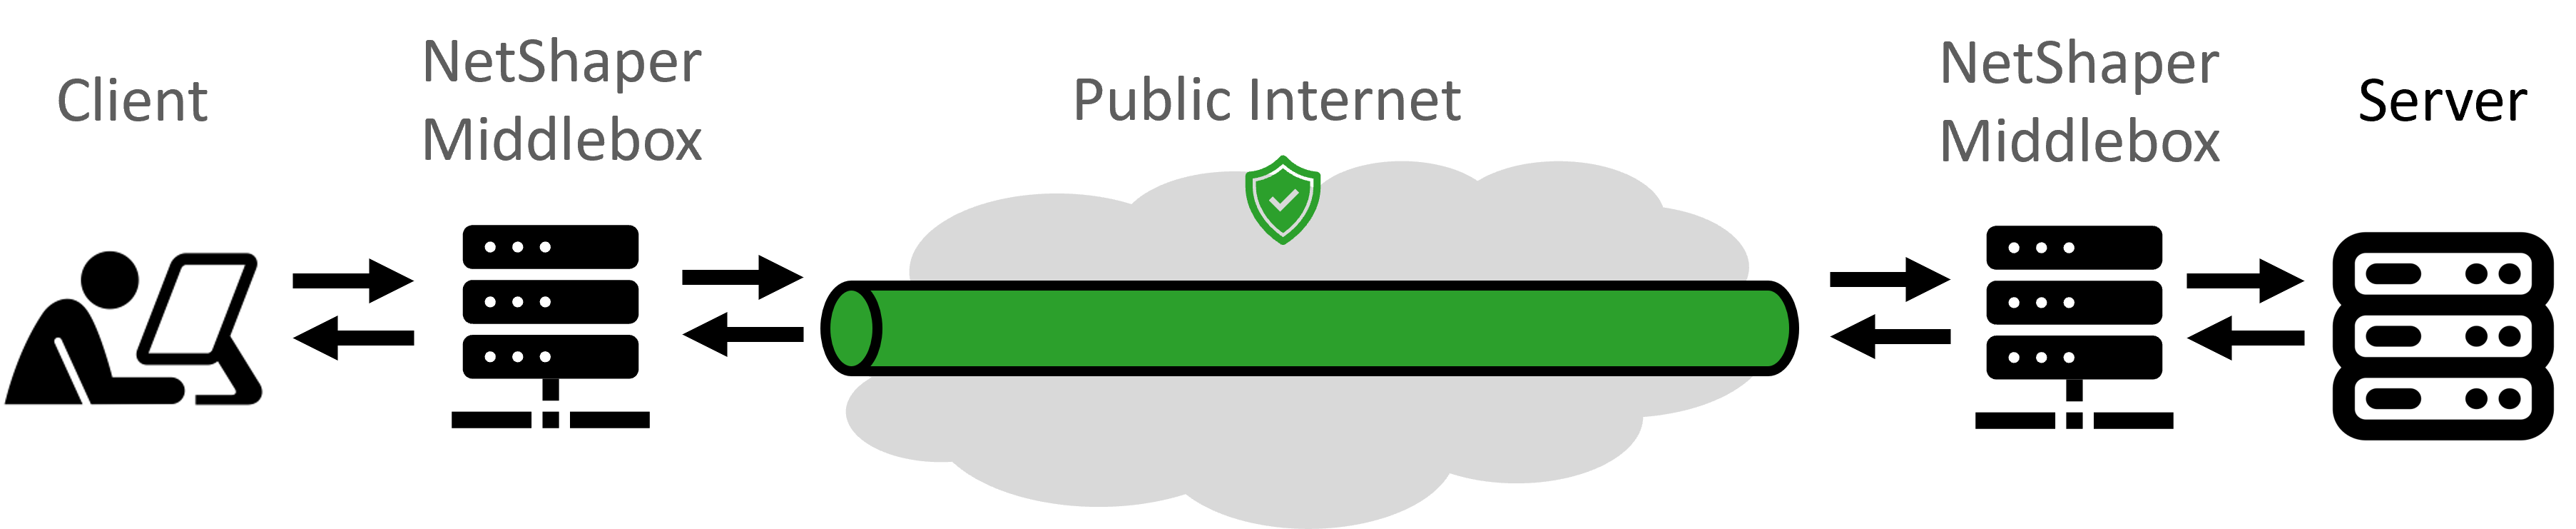
\includegraphics[width=\columnwidth]{figures/netshaper/netshaper-setup.png}
    \caption{NetShaper's Tunnel Setup}
    \label{fig:netshaper-setup}
\end{figure}

We designed NetShaper as a modular system that can be deployed using a pair of middleboxes, forming a forward and reverse proxy pair (see \Cref{fig:netshaper-setup}). 
Here, we describe in detail the architecture of the proxy setup and defer the discussion regarding the design of the middlebox to \Cref{sec:mb-design}. 

When using NetShaper, all clients communicate with the servers using three piecewise connections: 
(\textit{i}) between the client and the client-side middlebox, 
(\textit{ii}) between the client-side middlebox and the server-side middlebox, and
(\textit{iii}) between the server-side middlebox and the server.

For connection \textit{i} and \textit{iii}, NetShaper relies on standard TCP/UDP protocols. However, for connection \textit{ii} (i.e. to proxy the payload), NetShaper utilises QUIC. 
Using QUIC to proxy the payload avoids the TCP meltdown problem [??] that occurs when tunnelling TCP via TCP.
In addition, using QUIC also avoids the problem of an observer/attacker being able to distinguish between payload and padding that would occur when TCP was tunnelled via UDP (as the end host would retransmit payload, but the padding would not be retransmitted).

\paragraph{Setup.}
In order to be able to proxy end host traffic via NetShaper, the middleboxes need to be configured. 
The middleboxes first establish an encrypted QUIC connection between them, with user-specified reliability semantics.
Once the QUIC connection is established, NetShaper initialises three types of QUIC streams: Control, Data (Payload), and Dummy (Padding).
One \textit{control} stream is used to transmit messages regarding connection establishment or termination by the end host.
One \textit{dummy} stream is used for adding padding to the payload whenever necessary, based on the output of $f_{DP}$
\footnote{We avoid the use of PADDING frames in QUIC as they do not elicit acknowledgements and hence are distinguishable from the payload \cite{quic_rfc}.}.

\paragraph{Supporting multiple end hosts.}
As we discussed in \Cref{sec:quic-bg}, QUIC supports multiple streams in the same connection.
Using this, NetShaper can proxy the payload of multiple end hosts through a single QUIC connection between a pair of middleboxes.

While QUIC can support arbitrary initialisation and termination of streams, each stream has an associated header, which would increase the total transmission size.
For example, when transmitting two bytes in a single stream, the total transmission size would be $2 + S_{header}$.
However, when transmitting two streams of one byte each, the total transmission size would be $2 + 2*S_{header}$. 
An adversary may be able to distinguish between these two scenarios.
In order to avoid such a situation, NetShaper fixes and initialises a fixed number of streams per QUIC connection during the setup phase.
NetShaper assigns an unused stream to the client whenever a new client connects to the middlebox.
Similarly, NetShaper marks a stream as unused when an end host terminates the connection.

\endinput
\section{Middlebox Design}
\label{sec:mb-design}

While it is possible to apply NetShaper framework's approach at any network layer, we chose to develop the system as an L4 (Transport Layer) proxy.
This enables the system to be easily deployable, entirely in userspace and without requiring any superuser privileges. 
Developing NetShaper at L2 (Data Link Layer) or L3 (Network Layer) would require the deployer to either have the ability to modify the OS kernel or deploy some form of kernel bypass.

\begin{figure}[!htb]
    \centering
    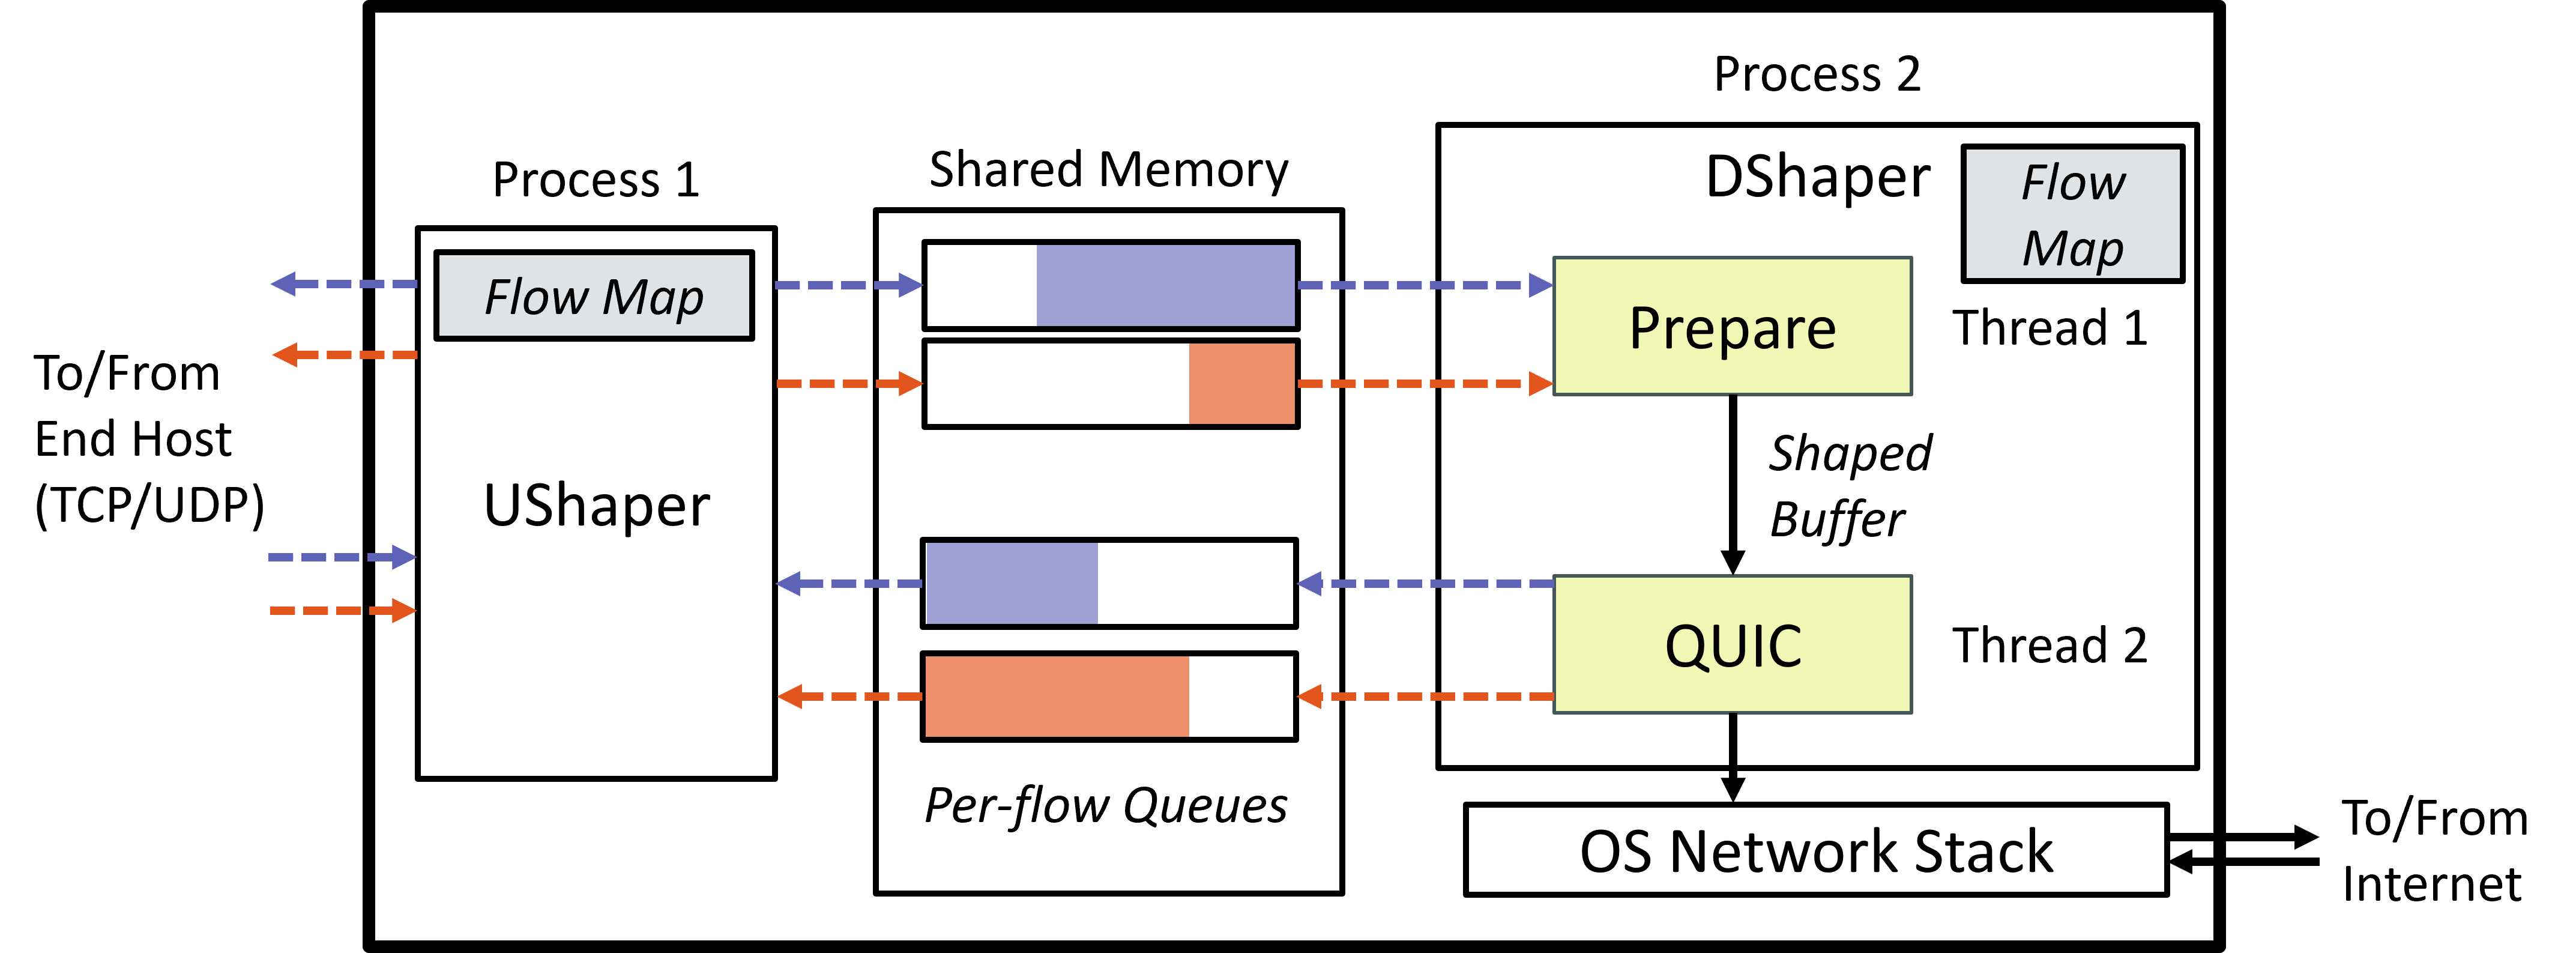
\includegraphics[width=\columnwidth]{figures/netshaper/middlebox-design.png}
    \caption{NetShaper Middlebox Design}
    \label{fig:middlebox-design}
\end{figure}

As outlined in \Cref{fig:middlebox-design}, NetShaper's middlebox consists of two main processes: UShaper and DShaper, and a shared memory between them.

\paragraph{UShaper.}
The \textit{UShaper} implements a client or a server to communicate with the end host.
It shares some Lamport Queues (LQs) [??] with DShaper.
It also consists of a flow map that maps a client with a corresponding pair of LQs.
\textit{UShaper} updates the flow map whenever a client establishes or terminates a connection.
In addition, it assigns an unused pair of LQs (one outbound and one inbound) to a new client and revokes that whenever the client terminates the connection.
The \textit{UShaper} receives outbound traffic from the end host and enqueues the payload in the assigned LQ.
Similarly, it dequeues inbound traffic from the inbound LQs and sends it to the corresponding end hosts.

\paragraph{DShaper.}
The \textit{DShaper} consists of two threads: \textit{Prepare} and \textit{QUIC worker}, and a flow map.
The flow map maps an LQ with a pre-initialised QUIC stream.
The \textit{Prepare} thread also measures the data available in the outbound LQs at the start of the window $W$.
It then adds noise to this available size based on the DP parameters.
Finally, it enqueues the payload and padding that needs to be transmitted.
The \textit{QUIC worker} transmits the enqueued data out to the network.
It also processes the received data, places it in the relevant LQ, and updates the flow map whenever a client initialises or terminates a connection.

In order to ensure that the operation of \textit{UShaper}, \textit{Prepare}, and \textit{QUIC worker} do not interfere with each other, we apply a few constraints in the implementation, and during the deployment of NetShaper.
First, all three components are required to be pinned on separate cores so that the execution time of one may not impact the others.
Second, in order to not leak the size of the payload due to the processing time of the enqueue operation done by the \textit{Prepare} thread, the \textit{Prepare} thread applies a lock for a fixed duration, during which the \textit{QUIC worker} can not transmit the data. 
We have outlined pseudo-code for both prepare and QUIC worker in \Cref{lst:prepare_and_worker}.
Finally, when receiving data, the \textit{QUIC worker} also enqueues the dummy bytes to a designated LQ so that the processing time remains consistent with the size of the data (see Figure ??).

\paragraph{Shared Memory.}
Both \textit{UShaper} and \textit{DShaper} have a shared memory between them.
This shared memory consists of three types of LQs: Control, Payload, Dummy
Similar to the stream types outlined in \Cref{sec:proxy-arch}, \textit{Control} LQ transmits the information about a connection establishment or termination by a client. 
\textit{Payload} LQ consists of the bytes received from the end host or to be sent to the end host.
\textit{Dummy} LQ consists of the dummy/padding bytes that are received.

\begin{minipage}{\textwidth}
\lstinputlisting[language=Python]{code/netshaper/prepare_and_worker.py}
\captionsetup{type=lstlisting}
\caption{Prepare and QUIC Worker Pseudo-code}
\label{lst:prepare_and_worker}
\end{minipage}

\endinput


\begin{figure}[!htb]
    \centering
    
\includegraphics[width=\columnwidth]{figures/netshaper/middlebox-design-overview.png}
    \caption{Overview of NetShaper's Middlebox}
    \label{fig:middlebox-design-overview}
\end{figure}

\endinput

Should we add pseudo-codes for UShaper and DShaper?
\section{Performance}\label{sec:netshaper-performance}
\section{Limitations and Discussion}\label{sec:netshaper-discussion}

\endinput

\begin{singlespace}
\raggedright
\bibliographystyle{abbrvnat}
\bibliography{biblio}
\end{singlespace}

\end{document}

\title{Side-Channel Security in Networks: From the Internet to Interconnects}
%\subtitle{If you want a subtitle}

\author{Rut Vora}
\previousdegree{B. Engineering in Computer Science, BITS-Pilani, 2020}

% What is this dissertation for?
\degreetitle{Master of Science}

\institution{The University of British Columbia}
\campus{Vancouver}

\faculty{The Faculty of Graduate and Postdoctoral Studies}
\department{Computer Science}
\submissionmonth{March}
\submissionyear{2025}

% details of your examining committee
\examiningcommittee{Aastha Mehta, Assistant Professor, Computer Science, \textsc{UBC}}{Supervisor}
% \examiningcommittee{Mathias L\'{e}cuyer, Assistant Professor, Computer Science, \textsc{UBC}}{Co-Supervisor}
% \examiningcommittee{Margo Seltzer, Professor, Computer Science, \textsc{UBC}}{Supervisory Committee Member}

%% hyperref package provides support for embedding meta-data in .PDF
%% files
\hypersetup{
  pdftitle={Side-Channel Security in Networks: From the Internet to Interconnects  (DRAFT: \today)},
  pdfauthor={Rut Vora},
  pdfkeywords={PCIe, CXL, Side Channels, Networks, Proxy}
}

%%%%%%%%%%%%%%%%%%%%%%%%%%%%%%%%%%%%%%%%%%%%%%%%%%%%%%%%%%%%%%%%%%%%%%
%%%%%%%%%%%%%%%%%%%%%%%%%%%%%%%%%%%%%%%%%%%%%%%%%%%%%%%%%%%%%%%%%%%%%%
%% 
%% The document content
%%

%% LaTeX's \includeonly commands causes any uses of \include{} to only
%% include files that are in the list.  This is helpful to produce
%% subsets of your thesis (e.g., for committee members who want to see
%% the dissertation chapter by chapter).  It also saves time by 
%% avoiding reprocessing the entire file.
%\includeonly{intro,conclusions}
%\includeonly{discussion}

\begin{document}

%%%%%%%%%%%%%%%%%%%%%%%%%%%%%%%%%%%%%%%%%%%%%%%%%%
%% From Thesis Components: Tradtional Thesis
%% <http://www.grad.ubc.ca/current-students/dissertation-thesis-preparation/order-components>

% Preliminary Pages (numbered in lower case Roman numerals)
%    1. Title page (mandatory)
\maketitle

%    2. Committee page (mandatory): lists supervisory committee and,
%    if applicable, the examining committee
\makecommitteepage

%    3. Abstract (mandatory - maximum 350 words)
%% The following is a directive for TeXShop to indicate the main file
%%!TEX root = diss.tex

\chapter{Abstract}

This document provides brief instructions for using the \class{ubcdiss}
class to write a \acs{UBC}-conformant dissertation in \LaTeX.  This
document is itself written using the \class{ubcdiss} class and is
intended to serve as an example of writing a dissertation in \LaTeX.
This document has embedded \acp{URL} and is intended to be viewed
using a computer-based \ac{PDF} reader.

Note: Abstracts should generally try to avoid using acronyms.

Note: at \ac{UBC}, both the \ac{GPS} Ph.D. defence programme and the
Library's online submission system restricts abstracts to 350
words.

\ifgpscopy
  This document was typeset in \texttt{gpscopy} mode.
\else
  This document was typeset in non-\texttt{gpscopy} mode.
\fi

% Consider placing version information if you circulate multiple drafts
%\vfill
%\begin{center}
%\begin{sf}
%\fbox{Revision: \today}
%\end{sf}
%\end{center}

\cleardoublepage

%    4. Lay Summary (Effective May 2017, mandatory - maximum 150 words)
\chapter{Lay Summary}

% Limit to 150-ish words

\paragraph{} Communication networks, whether the internet or hardware interconnects like PCIe (which connect components inside a computer), play a crucial role in modern computing. 
Although they operate at different levels, both are used to transfer data and can be vulnerable to side-channel attacks, which leak unintended information.

This research looks at security risks in both types of networks and explores their similarities. 
The first part focuses on reducing side-channel attacks in internet-like networks with a scalable solution that allows users to balance security with performance trade-offs like latency and bandwidth. 
The second part examines whether similar attacks can happen in PCIe interconnects.

By drawing similarities between the two types of attacks, we provide a unified perspective on securing communication networks against side-channel threats.

\cleardoublepage

%    5. Preface
%% The following is a directive for TeXShop to indicate the main file
%%!TEX root = diss.tex

\chapter{Preface}

At \ac{UBC}, a preface may be required.  Be sure to check the
\ac{GPS} guidelines as they may have specific content to be included.

\cleardoublepage

%    6. Table of contents (mandatory - list all items in the preliminary pages
%    starting with the abstract, followed by chapter headings and
%    subheadings, bibliographies and appendices)
\tableofcontents
\cleardoublepage	% required by tocloft package

%    7. List of tables (mandatory if thesis has tables)
\listoftables
\cleardoublepage	% required by tocloft package

%    8. List of figures (mandatory if thesis has figures)
\listoffigures
\cleardoublepage	% required by tocloft package

%    9. List of illustrations (mandatory if thesis has illustrations)
%   10. Lists of symbols, abbreviations or other (optional)

%   11. Glossary (optional)
\input{glossary}	% always input, since other macros may rely on it

\textspacing		% begin one-half or double spacing

%   12. Acknowledgements (optional)
%% The following is a directive for TeXShop to indicate the main file
%%!TEX root = thesis.tex

\chapter{Acknowledgments}

I would like to express my deepest gratitude to my advisor, Prof. Aastha Mehta, whose unwavering support, invaluable guidance, and expertise have been instrumental in shaping this dissertation.
Their dedication to mentoring, insightful feedback, and commitment to pushing the boundaries of my knowledge have been the driving forces behind this research endeavour. 

I would like to convey my sincerest appreciation to my collaborators, Amir Sabzi, Satvik Vemuganti, Arun Balamurali and Lucas Qin, whose tireless efforts have been indispensable throughout this project.

I would like to express my sincere gratitude to all members of the Systopia lab for their valuable ideas, discussions, and support throughout this work. Their insights and encouragement have been instrumental in refining concepts and overcoming challenges. The collaborative environment and shared knowledge have significantly contributed to the progress of this research.

\endinput

I extend my heartfelt gratitude to Prof. Margo Seltzer for her invaluable contributions as a committee member for this dissertation.
Her extensive knowledge and keen insights have greatly enriched the depth and quality of this work.

%   13. Dedication (optional)

% Body of Thesis (not all sections may apply)
\mainmatter

\acresetall	% reset all acronyms used so far

% Main Sections
%% The following is a directive for TeXShop to indicate the main file
%%!TEX root = diss.tex

\chapter{Introduction}
\label{ch:Introduction}

\begin{epigraph}
    \emph{If I have seen farther it is by standing on the shoulders of
    Giants.} ---~Sir Isaac Newton (1855)
\end{epigraph}

This document provides a quick set of instructions for using the
\class{ubcdiss} class to write a dissertation in \LaTeX. 
Unfortunately this document cannot provide an introduction to using
\LaTeX.  The classic reference for learning \LaTeX\ is
\citeauthor{lamport-1994-ladps}'s
book~\cite{lamport-1994-ladps}.  There are also many freely-available
tutorials online;
\webref{http://www.andy-roberts.net/misc/latex/}{Andy Roberts' online
    \LaTeX\ tutorials}
seems to be excellent.
The source code for this docment, however, is intended to serve as
an example for creating a \LaTeX\ version of your dissertation.

We start by discussing organizational issues, such as splitting
your dissertation into multiple files, in
\autoref{sec:SuggestedThesisOrganization}.
We then cover the ease of managing cross-references in \LaTeX\ in
\autoref{sec:CrossReferences}.
We cover managing and using bibliographies with \BibTeX\ in
\autoref{sec:BibTeX}. 
We briefly describe typesetting attractive tables in
\autoref{sec:TypesettingTables}.
We briefly describe including external figures in
\autoref{sec:Graphics}, and using special characters and symbols
in \autoref{sec:SpecialSymbols}.
As it is often useful to track different versions of your dissertation,
we discuss revision control further in
\autoref{sec:DissertationRevisionControl}. 
We conclude with pointers to additional sources of information in
\autoref{sec:Conclusions}.

%%%%%%%%%%%%%%%%%%%%%%%%%%%%%%%%%%%%%%%%%%%%%%%%%%%%%%%%%%%%%%%%%%%%%%
\section{Suggested Thesis Organization}
\label{sec:SuggestedThesisOrganization}

The \acs{UBC} \acf{GPS} specifies a particular arrangement of the
components forming a thesis.\footnote{See
    \url{http://www.grad.ubc.ca/current-students/dissertation-thesis-preparation/order-components}}
This template reflects that arrangement.

In terms of writing your thesis, the recommended best practice for
organizing large documents in \LaTeX\ is to place each chapter in
a separate file.  These chapters are then included from the main
file through the use of \verb+\include{file}+.  A thesis might
be described as six files such as \file{intro.tex},
\file{relwork.tex}, \file{model.tex}, \file{eval.tex},
\file{discuss.tex}, and \file{concl.tex}.

We also encourage you to use macros for separating how something
will be typeset (\eg bold, or italics) from the meaning of that
something. 
For example, if you look at \file{intro.tex}, you will see repeated
uses of a macro \verb+\file{}+ to indicate file names.
The \verb+\file{}+ macro is defined in the file \file{macros.tex}.
The consistent use of \verb+\file{}+ throughout the text not only
indicates that the argument to the macro represents a file (providing
meaning or semantics), but also allows easily changing how
file names are typeset simply by changing the definition of the
\verb+\file{}+ macro.
\file{macros.tex} contains other useful macros for properly typesetting
things like the proper uses of the latinate \emph{exempli grati\={a}}
and \emph{id est} (\ie \verb+\eg+ and \verb+\ie+), 
web references with a footnoted \acs{URL} (\verb+\webref{url}{text}+),
as well as definitions specific to this documentation
(\verb+\latexpackage{}+).

%%%%%%%%%%%%%%%%%%%%%%%%%%%%%%%%%%%%%%%%%%%%%%%%%%%%%%%%%%%%%%%%%%%%%%
\section{Making Cross-References}
\label{sec:CrossReferences}

\LaTeX\ make managing cross-references easy, and the \latexpackage{hyperref}
package's\ \verb+\autoref{}+ command\footnote{%
    The \latexpackage{hyperref} package is included by default in this
    template.}
makes it easier still. 

A thing to be cross-referenced, such as a section, figure, or equation,
is \emph{labelled} using a unique, user-provided identifier, defined
using the \verb+\label{}+ command.  
The thing is referenced elsewhere using the \verb+\autoref{}+ command.
For example, this section was defined using:
\begin{lstlisting}
    \section{Making Cross-References}
    \label{sec:CrossReferences}
\end{lstlisting}
References to this section are made as follows:
\begin{lstlisting}
    We then cover the ease of managing cross-references in \LaTeX\
    in \autoref{sec:CrossReferences}.
\end{lstlisting}
\verb+\autoref{}+ takes care of determining the \emph{type} of the 
thing being referenced, so the example above is rendered as
\begin{quote}
    We then cover the ease of managing cross-references in \LaTeX\
    in \autoref{sec:CrossReferences}.
\end{quote}

The label is any simple sequence of characters, numbers, digits,
and some punctuation marks such as ``:'' and ``--''; there should
be no spaces.  Try to use a consistent key format: this simplifies
remembering how to make references.  This document uses a prefix
to indicate the type of the thing being referenced, such as \texttt{sec}
for sections, \texttt{fig} for figures, \texttt{tbl} for tables,
and \texttt{eqn} for equations.

For details on defining the text used to describe the type
of \emph{thing}, search \file{diss.tex} and the \latexpackage{hyperref}
documentation for \texttt{autorefname}.


%%%%%%%%%%%%%%%%%%%%%%%%%%%%%%%%%%%%%%%%%%%%%%%%%%%%%%%%%%%%%%%%%%%%%%
\section{Managing Bibliographies with \BibTeX}
\label{sec:BibTeX}

One of the primary benefits of using \LaTeX\ is its companion program,
\BibTeX, for managing bibliographies and citations.  Managing
bibliographies has three parts: (i) describing references,
(ii)~citing references, and (iii)~formatting cited references.

\subsection{Describing References}

\BibTeX\ defines a standard format for recording details about a
reference.  These references are recorded in a file with a
\file{.bib} extension.  \BibTeX\ supports a broad range of
references, such as books, articles, items in a conference proceedings,
chapters, technical reports, manuals, dissertations, and unpublished
manuscripts. 
A reference may include attributes such as the authors,
the title, the page numbers, the \ac{DOI}, or a \ac{URL}.  A reference
can also be augmented with personal attributes, such as a rating,
notes, or keywords.

Each reference must be described by a unique \emph{key}.\footnote{%
    Note that the citation keys are different from the reference
    identifiers as described in \autoref{sec:CrossReferences}.}
A key is a simple sequence of characters, numbers, digits, and some
punctuation marks such as ``:'' and ``--''; there should be no spaces. 
A consistent key format simiplifies remembering how to make references. 
For example:
\begin{quote}
   \fbox{\emph{last-name}}\texttt{-}\fbox{\emph{year}}\texttt{-}\fbox{\emph{contracted-title}}
\end{quote}
where \emph{last-name} represents the last name for the first author,
and \emph{contracted-title} is some meaningful contraction of the
title.  Then \citeauthor{kiczales-1997-aop}'s seminal article on
aspect-oriented programming~\cite{kiczales-1997-aop} (published in
\citeyear{kiczales-1997-aop}) might be given the key
\texttt{kiczales-1997-aop}.

An example of a \BibTeX\ \file{.bib} file is included as
\file{biblio.bib}.  A description of the format a \file{.bib}
file is beyond the scope of this document.  We instead encourage
you to use one of the several reference managers that support the
\BibTeX\ format such as
\webref{http://jabref.sourceforge.net}{JabRef} (multiple platforms) or
\webref{http://bibdesk.sourceforge.net}{BibDesk} (MacOS\,X only). 
These front ends are similar to reference managers such as
EndNote or RefWorks.


\subsection{Citing References}

Having described some references, we then need to cite them.  We
do this using a form of the \verb+\cite+ command.  For example:
\begin{lstlisting}
    \citet{kiczales-1997-aop} present examples of crosscutting 
    from programs written in several languages.
\end{lstlisting}
When processed, the \verb+\citet+ will cause the paper's authors
and a standardized reference to the paper to be inserted in the
document, and will also include a formatted citation for the paper
in the bibliography.  For example:
\begin{quote}
    \citet{kiczales-1997-aop} present examples of crosscutting 
    from programs written in several languages.
\end{quote}
There are several forms of the \verb+\cite+ command (provided
by the \latexpackage{natbib} package), as demonstrated in
\autoref{tbl:natbib:cite}.
Note that the form of the citation (numeric or author-year) depends
on the bibliography style (described in the next section).
The \verb+\citet+ variant is used when the author names form
an object in the sentence, whereas the \verb+\citep+ variant
is used for parenthetic references, more like an end-note.
Use \verb+\nocite+ to include a citation in the bibliography
but without an actual reference.
\nocite{rowling-1997-hpps}
\begin{table}
\caption[Available \texttt{cite} variants]{%
    Available \texttt{cite} variants; the exact citation style
    depends on whether the bibliography style is numeric or author-year.}
\label{tbl:natbib:cite}
\centering
\begin{tabular}{lp{3.25in}}\toprule
Variant & Result \\
\midrule
% We cheat here to simulate the cite/citep/citet for APA-like styles
\verb+\cite+ & Parenthetical citation (\eg ``\cite{kiczales-1997-aop}''
    or ``(\citeauthor{kiczales-1997-aop} \citeyear{kiczales-1997-aop})'') \\
\verb+\citet+ & Textual citation: includes author (\eg
    ``\citet{kiczales-1997-aop}'' or
    or ``\citeauthor{kiczales-1997-aop} (\citeyear{kiczales-1997-aop})'') \\
\verb+\citet*+ & Textual citation with unabbreviated author list \\
\verb+\citealt+ & Like \verb+\citet+ but without parentheses \\
\verb+\citep+ & Parenthetical citation (\eg ``\cite{kiczales-1997-aop}''
    or ``(\citeauthor{kiczales-1997-aop} \citeyear{kiczales-1997-aop})'') \\
\verb+\citep*+ & Parenthetical citation with unabbreviated author list \\
\verb+\citealp+ & Like \verb+\citep+ but without parentheses \\
\verb+\citeauthor+ & Author only (\eg ``\citeauthor{kiczales-1997-aop}'') \\
\verb+\citeauthor*+ & Unabbreviated authors list 
    (\eg ``\citeauthor*{kiczales-1997-aop}'') \\
\verb+\citeyear+ & Year of citation (\eg ``\citeyear{kiczales-1997-aop}'') \\
\bottomrule
\end{tabular}
\end{table}

\subsection{Formatting Cited References}

\BibTeX\ separates the citing of a reference from how the cited
reference is formatted for a bibliography, specified with the
\verb+\bibliographystyle+ command. 
There are many varieties, such as \texttt{plainnat}, \texttt{abbrvnat},
\texttt{unsrtnat}, and \texttt{vancouver}.
This document was formatted with \texttt{abbrvnat}.
Look through your \TeX\ distribution for \file{.bst} files. 
Note that use of some \file{.bst} files do not emit all the information
necessary to properly use \verb+\citet{}+, \verb+\citep{}+,
\verb+\citeyear{}+, and \verb+\citeauthor{}+.

There are also packages available to place citations on a per-chapter
basis (\latexpackage{bibunits}), as footnotes (\latexpackage{footbib}),
and inline (\latexpackage{bibentry}).
Those who wish to exert maximum control over their bibliography
style should see the amazing \latexpackage{custom-bib} package.

%%%%%%%%%%%%%%%%%%%%%%%%%%%%%%%%%%%%%%%%%%%%%%%%%%%%%%%%%%%%%%%%%%%%%%
\section{Typesetting Tables}
\label{sec:TypesettingTables}

\citet{lamport-1994-ladps} made one grievous mistake
in \LaTeX: his suggested manner for typesetting tables produces
typographic abominations.  These suggestions have unfortunately
been replicated in most \LaTeX\ tutorials.  These
abominations are easily avoided simply by ignoring his examples
illustrating the use of horizontal and vertical rules (specifically
the use of \verb+\hline+ and \verb+|+) and using the
\latexpackage{booktabs} package instead.

The \latexpackage{booktabs} package helps produce tables in the form
used by most professionally-edited journals through the use of
three new types of dividing lines, or \emph{rules}.
% There are times that you don't want to use \autoref{}
Tables~\ref{tbl:natbib:cite} and~\ref{tbl:LaTeX:Symbols} are two
examples of tables typeset with the \latexpackage{booktabs} package.
The \latexpackage{booktabs} package provides three new commands
for producing rules:
\verb+\toprule+ for the rule to appear at the top of the table,
\verb+\midrule+ for the middle rule following the table header,
and \verb+\bottomrule+ for the bottom-most at the end of the table.
These rules differ by their weight (thickness) and the spacing before
and after.
A table is typeset in the following manner:
\begin{lstlisting}
    \begin{table}
    \caption{The caption for the table}
    \label{tbl:label}
    \centering
    \begin{tabular}{cc}
    \toprule
    Header & Elements \\
    \midrule
    Row 1 & Row 1 \\
    Row 2 & Row 2 \\
    % ... and on and on ...
    Row N & Row N \\
    \bottomrule
    \end{tabular}
    \end{table}
\end{lstlisting}
See the \latexpackage{booktabs} documentation for advice in dealing with
special cases, such as subheading rules, introducing extra space
for divisions, and interior rules.

%%%%%%%%%%%%%%%%%%%%%%%%%%%%%%%%%%%%%%%%%%%%%%%%%%%%%%%%%%%%%%%%%%%%%%
\section{Figures, Graphics, and Special Characters}
\label{sec:Graphics}

Most \LaTeX\ beginners find figures to be one of the more challenging
topics.  In \LaTeX, a figure is a \emph{floating element}, to be
placed where it best fits.
The user is not expected to concern him/herself with the placement
of the figure.  The figure should instead be labelled, and where
the figure is used, the text should use \verb+\autoref+ to reference
the figure's label.
\autoref{fig:latex-affirmation} is an example of a figure.
\begin{figure}
    \centering
    % For the sake of this example, we'll just use text
    %\includegraphics[width=3in]{file}
    \Huge{\textsf{\LaTeX\ Rocks!}}
    \caption{Proof of \LaTeX's amazing abilities}
    \label{fig:latex-affirmation}   % label should change
\end{figure}
A figure is generally included as follows:
\begin{lstlisting}
    \begin{figure}
    \centering
    \includegraphics[width=3in]{file}
    \caption{A useful caption}
    \label{fig:fig-label}   % label should change
    \end{figure}
\end{lstlisting}
There are three items of note:
\begin{enumerate}
\item External files are included using the \verb+\includegraphics+
    command.  This command is defined by the \latexpackage{graphicx} package
    and can often natively import graphics from a variety of formats.
    The set of formats supported depends on your \TeX\ command processor.
    Both \texttt{pdflatex} and \texttt{xelatex}, for example, can
    import \textsc{gif}, \textsc{jpg}, and \textsc{pdf}.  The plain
    version of \texttt{latex} only supports \textsc{eps} files.

\item The \verb+\caption+ provides a caption to the figure. 
    This caption is normally listed in the List of Figures; you
    can provide an alternative caption for the LoF by providing
    an optional argument to the \verb+\caption+ like so:
    \begin{lstlisting}
    \caption[nice shortened caption for LoF]{%
	longer detailed caption used for the figure}
    \end{lstlisting}
    \ac{GPS} generally prefers shortened single-line captions
    in the LoF: multiple-line captions are a bit unwieldy.

\item The \verb+\label+ command provides for associating a unique, user-defined,
    and descriptive identifier to the figure.  The figure can be
    can be referenced elsewhere in the text with this identifier
    as described in \autoref{sec:CrossReferences}.
\end{enumerate}
See Keith Reckdahl’s excellent guide for more details,
\webref{http://www.ctan.org/tex-archive/info/epslatex.pdf}{\emph{Using
imported graphics in LaTeX2e}}.

\section{Special Characters and Symbols}
\label{sec:SpecialSymbols}

\LaTeX\ appropriates many common symbols for its own purposes,
with some used for commands (\eg \verb+\{}&%+) and
mathematics (\eg \verb+$^_+), and others are automagically transformed
into typographically-preferred forms (\eg \verb+-`'+) or to
completely different forms (\eg \verb+<>+).
\autoref{tbl:LaTeX:Symbols} presents a list of common symbols and
their corresponding \LaTeX\ commands.  A much more comprehensive list 
of symbols and accented characters is available at:
\url{http://www.ctan.org/tex-archive/info/symbols/comprehensive/}
\begin{table}
\caption{Useful \LaTeX\ symbols}\label{tbl:LaTeX:Symbols}
\centering\begin{tabular}{ccp{0.5cm}cc}\toprule
\LaTeX & Result && \LaTeX & Result \\
\midrule
    \verb+\texttrademark+ & \texttrademark && \verb+\&+ & \& \\
    \verb+\textcopyright+ & \textcopyright && \verb+\{ \}+ & \{ \} \\
    \verb+\textregistered+ & \textregistered && \verb+\%+ & \% \\
    \verb+\textsection+ & \textsection && \verb+\verb!~!+ & \verb!~! \\
    \verb+\textdagger+ & \textdagger && \verb+\$+ & \$ \\
    \verb+\textdaggerdbl+ & \textdaggerdbl && \verb+\^{}+ & \^{} \\
    \verb+\textless+ & \textless && \verb+\_+ & \_ \\
    \verb+\textgreater+ & \textgreater && \\
\bottomrule
\end{tabular}
\end{table}

%%%%%%%%%%%%%%%%%%%%%%%%%%%%%%%%%%%%%%%%%%%%%%%%%%%%%%%%%%%%%%%%%%%%%%
\section{Changing Page Widths and Heights}

The \class{ubcdiss} class is based on the standard \LaTeX\ \class{book}
class~\cite{lamport-1994-ladps} that selects a line-width to carry
approximately 66~characters per line.  This character density is
claimed to have a pleasing appearance and also supports more rapid
reading~\cite{bringhurst-2002-teots}.  I would recommend that you
not change the line-widths!

\subsection{The \texttt{geometry} Package}

Some students are unfortunately saddled with misguided supervisors
or committee members whom believe that documents should have the
narrowest margins possible.  The \latexpackage{geometry} package is
helpful in such cases.  Using this package is as simple as:
\begin{lstlisting}
    \usepackage[margin=1.25in,top=1.25in,bottom=1.25in]{geometry}
\end{lstlisting}
You should check the package's documentation for more complex uses.

\subsection{Changing Page Layout Values By Hand}

There are some miserable students with requirements for page layouts
that vary throughout the document.  Unfortunately the
\latexpackage{geometry} can only be specified once, in the document's
preamble.  Such miserable students must set \LaTeX's layout parameters
by hand:
\begin{lstlisting}
    \setlength{\topmargin}{-.75in}
    \setlength{\headsep}{0.25in}
    \setlength{\headheight}{15pt}
    \setlength{\textheight}{9in}
    \setlength{\footskip}{0.25in}
    \setlength{\footheight}{15pt}

    % The *sidemargin values are relative to 1in; so the following
    % results in a 0.75 inch margin
    \setlength{\oddsidemargin}{-0.25in}
    \setlength{\evensidemargin}{-0.25in}
    \setlength{\textwidth}{7in}       % 1.1in margins (8.5-2*0.75)
\end{lstlisting}
These settings necessarily require assuming a particular page height
and width; in the above, the setting for \verb+\textwidth+ assumes
a \textsc{US} Letter with an 8.5'' width.
The \latexpackage{geometry} package simply uses the page height and
other specified values to derive the other layout values.
The
\href{http://tug.ctan.org/tex-archive/macros/latex/required/tools/layout.pdf}{\texttt{layout}}
package provides a
handy \verb+\layout+ command to show the current page layout
parameters. 


\subsection{Making Temporary Changes to Page Layout}

There are occasions where it becomes necessary to make temporary
changes to the page width, such as to accomodate a larger formula. 
The \latexmiscpackage{chngpage} package provides an \env{adjustwidth}
environment that does just this.  For example:
\begin{lstlisting}
    % Expand left and right margins by 0.75in
    \begin{adjustwidth}{-0.75in}{-0.75in}
    % Must adjust the perceived column width for LaTeX to get with it.
    \addtolength{\columnwidth}{1.5in}
    \[ an extra long math formula \]
    \end{adjustwidth}
\end{lstlisting}


%%%%%%%%%%%%%%%%%%%%%%%%%%%%%%%%%%%%%%%%%%%%%%%%%%%%%%%%%%%%%%%%%%%%%%
\section{Keeping Track of Versions with Revision Control}
\label{sec:DissertationRevisionControl}

Software engineers have used \acf{RCS} to track changes to their
software systems for decades.  These systems record the changes to
the source code along with context as to why the change was required.
These systems also support examining and reverting to particular
revisions from their system's past.

An \ac{RCS} can be used to keep track of changes to things other
than source code, such as your dissertation.  For example, it can
be useful to know exactly which revision of your dissertation was
sent to a particular committee member.  Or to recover an accidentally
deleted file, or a badly modified image.  With a revision control
system, you can tag or annotate the revision of your dissertation
that was sent to your committee, or when you incorporated changes
from your supervisor.

Unfortunately current revision control packages are not yet targetted
to non-developers.  But the Subversion project's
\webref{http://tortoisesvn.net/docs/release/TortoiseSVN_en/}{TortoiseSVN}
has greatly simplified using the Subversion revision control system
for Windows users.  You should consult your local geek.

A simpler alternative strategy is to create a GoogleMail account
and periodically mail yourself zipped copies of your dissertation.

%%%%%%%%%%%%%%%%%%%%%%%%%%%%%%%%%%%%%%%%%%%%%%%%%%%%%%%%%%%%%%%%%%%%%%
\section{Recommended Packages}

The real strength to \LaTeX\ is found in the myriad of free add-on
packages available for handling special formatting requirements.
In this section we list some helpful packages.

\subsection{Typesetting}

\begin{description}
\item[\latexpackage{enumitem}:]
    Supports pausing and resuming enumerate environments.

\item[\latexpackage{ulem}:]
    Provides two new commands for striking out and crossing out text
    (\verb+\sout{text}+ and \verb+\xout{text}+ respectively)
    The package should likely
    be used as follows:
    \begin{verbatim}
    \usepackage[normalem,normalbf]{ulem}
    \end{verbatim}
    to prevent the package from redefining the emphasis and bold fonts.

\item[\latexpackage{chngpage}:]
    Support changing the page widths on demand.

\item[\latexpackage{mhchem}:] 
    Support for typesetting chemical formulae and reaction equations.

\end{description}

Although not a package, the
\webref{http://www.ctan.org/tex-archive/support/latexdiff/}{\texttt{latexdiff}}
command is very useful for creating changebar'd versions of your
dissertation.


\subsection{Figures, Tables, and Document Extracts}

\begin{description}
\item[\latexpackage{pdfpages}:]
    Insert pages from other PDF files.  Allows referencing the extracted
    pages in the list of figures, adding labels to reference the page
    from elsewhere, and add borders to the pages.

\item[\latexpackage{subfig}:]
    Provides for including subfigures within a figure, and includes
    being able to separately reference the subfigures.  This is a
    replacement for the older \texttt{subfigure} environment.

\item[\latexpackage{rotating}:]
    Provides two environments, sidewaystable and sidewaysfigure,
    for typesetting tables and figures in landscape mode.  

\item[\latexpackage{longtable}:]
    Support for long tables that span multiple pages.

\item[\latexpackage{tabularx}:]
    Provides an enhanced tabular environment with auto-sizing columns.

\item[\latexpackage{ragged2e}:]
    Provides several new commands for setting ragged text (\eg forms
    of centered or flushed text) that can be used in tabular
    environments and that support hyphenation.

\end{description}


\subsection{Bibliography Related Packages}

\begin{description}
\item[\latexpackage{bibunits}:]
    Support having per-chapter bibliographies.

\item[\latexpackage{footbib}:]
    Cause cited works to be rendered using footnotes.

\item[\latexpackage{bibentry}:] 
    Support placing the details of a cited work in-line.

\item[\latexpackage{custom-bib}:]
    Generate a custom style for your bibliography.

\end{description}


%%%%%%%%%%%%%%%%%%%%%%%%%%%%%%%%%%%%%%%%%%%%%%%%%%%%%%%%%%%%%%%%%%%%%%
\section{Moving On}
\label{sec:Conclusions}

At this point, you should be ready to go.  Other handy web resources:
\begin{itemize}
\item \webref{http://www.ctan.org}{\ac{CTAN}} is \emph{the} comprehensive
    archive site for all things related to \TeX\ and \LaTeX. 
    Should you have some particular requirement, somebody else is
    almost certainly to have had the same requirement before you,
    and the solution will be found on \ac{CTAN}.  The links to
    various packages in this document are all to \ac{CTAN}.

\item An online
    \webref{http://www.ctan.org/get/info/latex2e-help-texinfo/latex2e.html}{%
	reference to \LaTeX\ commands} provides a handy quick-reference
    to the standard \LaTeX\ commands.

\item The list of 
    \webref{http://www.tex.ac.uk/cgi-bin/texfaq2html?label=interruptlist}{%
	Frequently Asked Questions about \TeX\ and \LaTeX}
    can save you a huge amount of time in finding solutions to
    common problems.

\item The \webref{http://www.tug.org/tetex/tetex-texmfdist/doc/}{te\TeX\
    documentation guide} features a very handy list of the most useful
    packages for \LaTeX\ as found in \ac{CTAN}.

\item The
\webref{http://www.ctan.org/tex-archive/macros/latex/required/graphics/grfguide.pdf}{\texttt{color}}
    package, part of the graphics bundle, provides handy commands
    for changing text and background colours.  Simply changing
    text to various levels of grey can have a very 
    \textcolor{greytext}{dramatic effect}.


\item If you're really keen, you might want to join the
    \webref{http://www.tug.org}{\TeX\ Users Group}.

\end{itemize}

\endinput

Any text after an \endinput is ignored.
You could put scraps here or things in progress.

\chapter{Background}

% We begin this chapter by discussing the problem of network side-channel attacks in \Cref{sec:ns-attacks}, in the context of two distinct applications: video streaming and web services.
% In \Cref{sec:dp-background}, we present a comprehensive definition of differential privacy (DP), outline its key properties, and highlight its primary applications, thereby setting the foundation for our differentially private traffic shaping mechanism.
% In \Cref{sec:background-quic} we provide a brief overview of the QUIC protocol, which plays a pivotal role in the design of {\sys}.
% Finally, in \Cref{sec:threat-model}, we conclude this chapter by explaining our threat model. 

\section{Network Side Channels}
\label{sec:network-side-channel-background}

Let us first understand how network side-channel attacks are carried out.
The ultimate goal of the attacker is to determine the contents of the web traffic being transmitted or received by the victim. More often than not, an attacker is interested in knowing if the victim accessed any content from a small subset and, if so, which content they accessed.
To do this, the attacker takes the following steps: 
1) Collect network traces
2) Build a classifier trained on the collected network traces
3) Gain access to the network shared with the victim
4) Profile the victim's network traffic
5) Determine whether the victim accessed any content of interest to the attacker

First, the attacker builds a collection of the content (e.g. webpages and video streams) that they are interested in. 
They collect network traces for this content under various network conditions to account for variability caused by the network itself. 
Then, the attacker trains a classifier on this collected network trace.
The classifier can use multiple features like packer sizes, inter-packer timing, total bytes transferred in a burst of packets, the duration of the burst and the interval between bursts, and the direction of the bursts \cite{schuster2017beautyburst}.

Next, the attacker infiltrates a machine that shares some network path with the victim.
This machine could also be the victim's machine. 
The malicious application could be a javascript-based advertisement on the page the victim is visiting or another process on the victim's machine, thus sharing the network card on that machine. 
It could also be a shared router/switch in the victim's network path to the server.
The attacker could either be another client connected to the same shared router/switch or someone who owns the router/switch.
If the attacker owns an element in the network path, they can directly observe all the features necessary to carry out the attack. 
Otherwise, they create congestion in the shared network path such that the victim's network traffic would contend with the attacker's traffic.
In this case, the attacker's traffic would be delayed, and the delay would be proportional to the victim's traffic, thus revealing some features of the victim's traffic.

The attacker collects the network traces of its own traffic and, based on that, extracts the features of the victim's traffic flow. These extracted features are then run through the pre-trained classifier, which helps the attacker determine which content the victim accessed. \citeauthor{schuster2017beautyburst} demonstrated that one could train a Convolution Neural Network (CNN)-based classifier to determine which video the victim is streaming. Similarly, prior work has demonstrated that such a network side channel-based approach can also be used to determine which webpage the victim is visiting \cite{hayes2016kfp, panchenko2016website, gong2010fingerprinting}

% \section{Threat Model}\label{sec:nsc-threat-model}

\section{NetShaper - Framework}
\label{sec:netshaper-framework-bg}

NetShaper \cite{sabzi2024netshaper} is both the name of a differential-privacy-based framework for mitigating network side-channel attacks and the system that utilises that framework. 
Here, we provide a brief description of the NetShaper Framework.

\subsection{Differential Privacy}
NetShaper's framework relies on Differential Privacy (DP) to provide robust, mathematical guarantees against side-channel attacks in internet networks.
DP is a framework originally proposed by \citeauthor{dwork2006differential} for releasing usable aggregate metrics regarding a dataset while limiting the leakage of information about individual data points in that dataset.
In other words, DP bounds the probability of an observer being able to infer if an individual data point was used to generate the aggregate metric the observer has access to.
DP has two main parameters: \\
\textbf{$\epsilon$: } Intuitively, it specifies the amount of privacy loss
\textbf{$\delta$: } Intuitively, it specifies the probability with which a given differentially-private mechanism can fail.


\begin{definition}[Differential privacy]
  \label{def:dp}
  A randomized algorithm $A_{DP}$ is $(\varepsilon, \delta)-DP$ if for all ${S} \subseteq Range(A_{DP})$ and for all datasets $D, D'$ that differ on a single element, we have:
  \begin{equation*}
    \Pr[A_{DP}(D) \in S] \leq \exp(\varepsilon)\Pr[A{DP}(D') \in S] + \delta
  \end{equation*}
\end{definition}

For any aggregate algorithm $A$, we can make an $(\varepsilon, \delta)-DP$ algorithm by adding some noise to the output of $A$.
There are many different mechanisms to add the noise $\eta$, but most commonly, $\eta$ is a function of $\varepsilon, \delta$ and other dataset-dependent parameters. 
Mathematically, $A_{DP}(D) = A(D) + \eta(\varepsilon, \delta, ...)$

DP has a few useful properties: 
\textbf{1) Post Processing:} Any further operations or processing on the output of an $(\varepsilon, \delta)-DP$ algorithm is also $(\varepsilon, \delta)-DP$.
This condition holds true as long as the operations carried out do not involve any auxiliary knowledge of the dataset.
\textbf{2) Composition:} It is possible to quantify the total privacy loss when multiple queries are issued to the same $(\varepsilon, \delta)-DP$ algorithm.

\subsection{Applying DP on network streams}
NetShaper uses DP to mitigate network side-channel attacks. 
To achieve this, NetShaper relies on two key ideas: 
First, NetShaper represents network traffic streams as datasets to which DP can be applied.
As DP applies to datasets, we must first represent a network stream as a dataset.
A network stream $S$ can be represented as a sequence of packets $P_i^S$, where each packet is associated with its length and the timestamp at which it was encountered (i.e. $P_i^S = (l_i^S, t_i^S$).
Hence, $S$ is the dataset consisting of the traffic shape, which can be used by an attacker to carry out a side-channel attack, as outlined in \Cref{sec:network-side-channel-background}.
As the network stream can potentially be long, NetShaper models the DP guarantees in windows of fixed length $W$ and can use composition to calculate the privacy loss across multiple windows.
Second, NetShaper relies on a buffering queue to control the shape of the traffic visible to the attacker within each window $W$ by discretising time into $W$-sized windows.
At the beginning of each discrete window, NetShaper checks the size of the buffer and adds DP noise to the size to determine the amount of data to be sent out in that window.


So, initially, the attacker was able to query a function $f(S, t_{start}, t_{end})$ to obtain the size and time of the packet that was transmitted by the victim. 
However, with the application of DP on the network stream, the attacker can now only query a new function $f_{DP}(S, t_{start}, t_{end})$.
$f_{DP}$ is a differentially private function ensuring that the probability of leaking individual entries of the dataset is bounded, and where $t_{end} - t_{start} = kW, k \in N$.

\endinput

Note: Should we add stuff about sensitivity? (I don't think it's necessary for my thesis)
\section{The QUIC protocol}
\label{sec:quic-bg}

QUIC is a connection-oriented transport layer protocol that can be deployed on top of UDP.
It is now standardised under RFC 9000 \cite{quic_rfc}.
It provides many features which are similar to TCP, like flow control, loss recovery, and congestion control. 
However, it also alleviates some problems that TCP encounters.
For example, QUIC enforces encryption in the initial handshake, thus ensuring that all traffic is always encrypted.
In addition, a QUIC connection can consist of multiple dynamically created streams, each of which can act as an independent byte stream. 
This helps alleviate the problem of head-of-line blocking faced by TCP, ensuring that one blocked stream does not affect others.
Each stream has a unique header containing the stream ID and the stream type, among other information.
Multiple such streams, with their headers, can be a part of a single encrypted QUIC packet.
This ensures that an attacker can not determine the number of streams being transmitted in a QUIC packet just by observing the encrypted packet or traffic stream.


\endinput

\footnote{While QUIC has a PADDING frame, we don't use it, as a packet that only contains padding frames will not be re-transmitted in case of packet loss, thus revealing that it was a dummy packet.}


\section{Side Channels in Interconnects}
\label{sec:interconnect-sc-bg}
Conceptually, carrying out a side-channel interconnect is very similar to carrying out such an attack on internet networks. 
The attacker creates congestion on a buffer in the communication path between the host (CPU) and the peripheral (e.g. GPU) and observes their own delay.
This delay would be proportional to the amount of data transferred by the victim, which would help the attacker gain insight into the victim's traffic shape.

However, a few differences between interconnects and traditional networks make it challenging to implement such an attack. \\
\textit{First}, The bandwidth of interconnects like PCIe is at least an order of magnitude higher than that of internet networks.
While a typical bandwidth in an internet network may be 1-10Gbps ( = 0.125 - 1.25 GBps), PCIe 4.0 can operate at a rate of 32GBps.
The high bandwidth makes it non-trivial to saturate the PCIe link. \\
\textit{Second}, latency in PCIe is at least three orders of magnitude smaller than that of internet networks.
Typically, internet latency is measured in milliseconds, while PCIe latency is measured in microseconds.
The low latency makes it difficult for the attacker to measure the delays accurately. \\
\textit{Third}, unlike internet networks, PCIe does not extend outside the machine of the host CPU.
This further adds to the challenge that the attacker needs to co-locate with the victim application on the same machine. \\
\textit{Fourth}, the PCIe protocol has a fixed behaviour depending on the type of transaction. 
Most transaction types can not generate enough traffic to even come close to saturating the bandwidth of PCIe. 
While saturating the bandwidth may not be necessary to create a side-channel attack, it would be useful if there is always at least one attacker packet in the buffer whenever the victim might transmit.
This would ensure that the attacker can observe a delay in their own packets for each packet or set of packets the victim transmits.

We provide a list of the transactions PCIe supports in \Cref{tab:pcie-transaction-types}, and a description of what each PCIe transaction type entails below: \\
\textbf{Posted:} Transactions where no response is issued or expected. 
These transactions are also asynchronous and hence allow multiple transactions of the same type to be in flight at the same time.\\
\textbf{Non-posted:} Transactions where a response is required. 
These types of transactions are also synchronous.
As such, one can not execute multiple of these simultaneously.\\
\textbf{Completions:} The completion of a previous non-posted transaction.\\

\begin{table}[htb]
    \centering
    \begin{tabular}{|l|l|p{0.65\textwidth}|}
        \hline
        \textbf{Transaction} & \textbf{Type} & \textbf{Description} \\ 
        \hline
        Memory Read  & Non-Posted & Read from a memory-mapped address space \\ 
        Memory Write & Posted     & Write to a memory-mapped address space  \\ 
        I/O Read     & Non-Posted & (Legacy PCI) Read from the I/O address space \\ 
        I/O Write    & Non-Posted & (Legacy PCI) Write to the I/O address space \\ 
        Config Read  & Non-Posted & Read control and status registers of the PCIe interface \\ 
        Config Write & Non-Posted & Write control and status registers of the PCIe interface \\  
        Message      & Posted     & Conveys additional information (e.g. Interrupts, Power Management, Error Signalling, Vendor-defined messaging). \\
        Completion   & Completion & Response to all non-posted transactions \\ 
        \hline
    \end{tabular}
    \caption{PCIe transaction types}
    \label{tab:pcie-transaction-types}
\end{table}


\subsection{Challenge: Measuring the time of PCIe transactions}

In \Cref{tab:pcie-transaction-types}, we can see that most PCIe transactions are Non-posted.
Only memory writes and messages are posted and hence asynchronous.
Asynchronous transactions such as a memory write (i.e. a \textit{store} instruction executed on memory-mapped PCIe endpoint memory region) would be more useful for carrying out a side-channel attack on PCIe.
This is because asynchronous transactions enable the attacker to have one transaction always pending to be sent out, regardless of the completion of the previous transaction(s).

However, measuring the completion time of an individual asynchronous transaction becomes more challenging as they are executed out-of-order. 
The naive solution of having a memory fence after each \textit{store} instruction would not work, as the memory fence would not allow the next \textit{store} instruction to be issued in parallel to the previous one, negating the benefit of using an asynchronous transaction.

\endinput




https://www.linkedin.com/pulse/pci-express-primer-3-transaction-layer-simon-southwell/
\section{AMD CPU Architecture}
\label{subsec:amd-arch-bg}

Modern CPUs consist of many components, such as execution units, caches, PCIe root complex, and DRAM controllers.
Some subset of these components is always traversed when data is sent to or from the CPU to the PCIe endpoints.
The behaviour of each individual component may impact how the side-channel attack is carried out.
As such, it becomes necessary to understand all the components that may be involved in a PCIe transaction.

\begin{figure}[!htb]
    \centering
    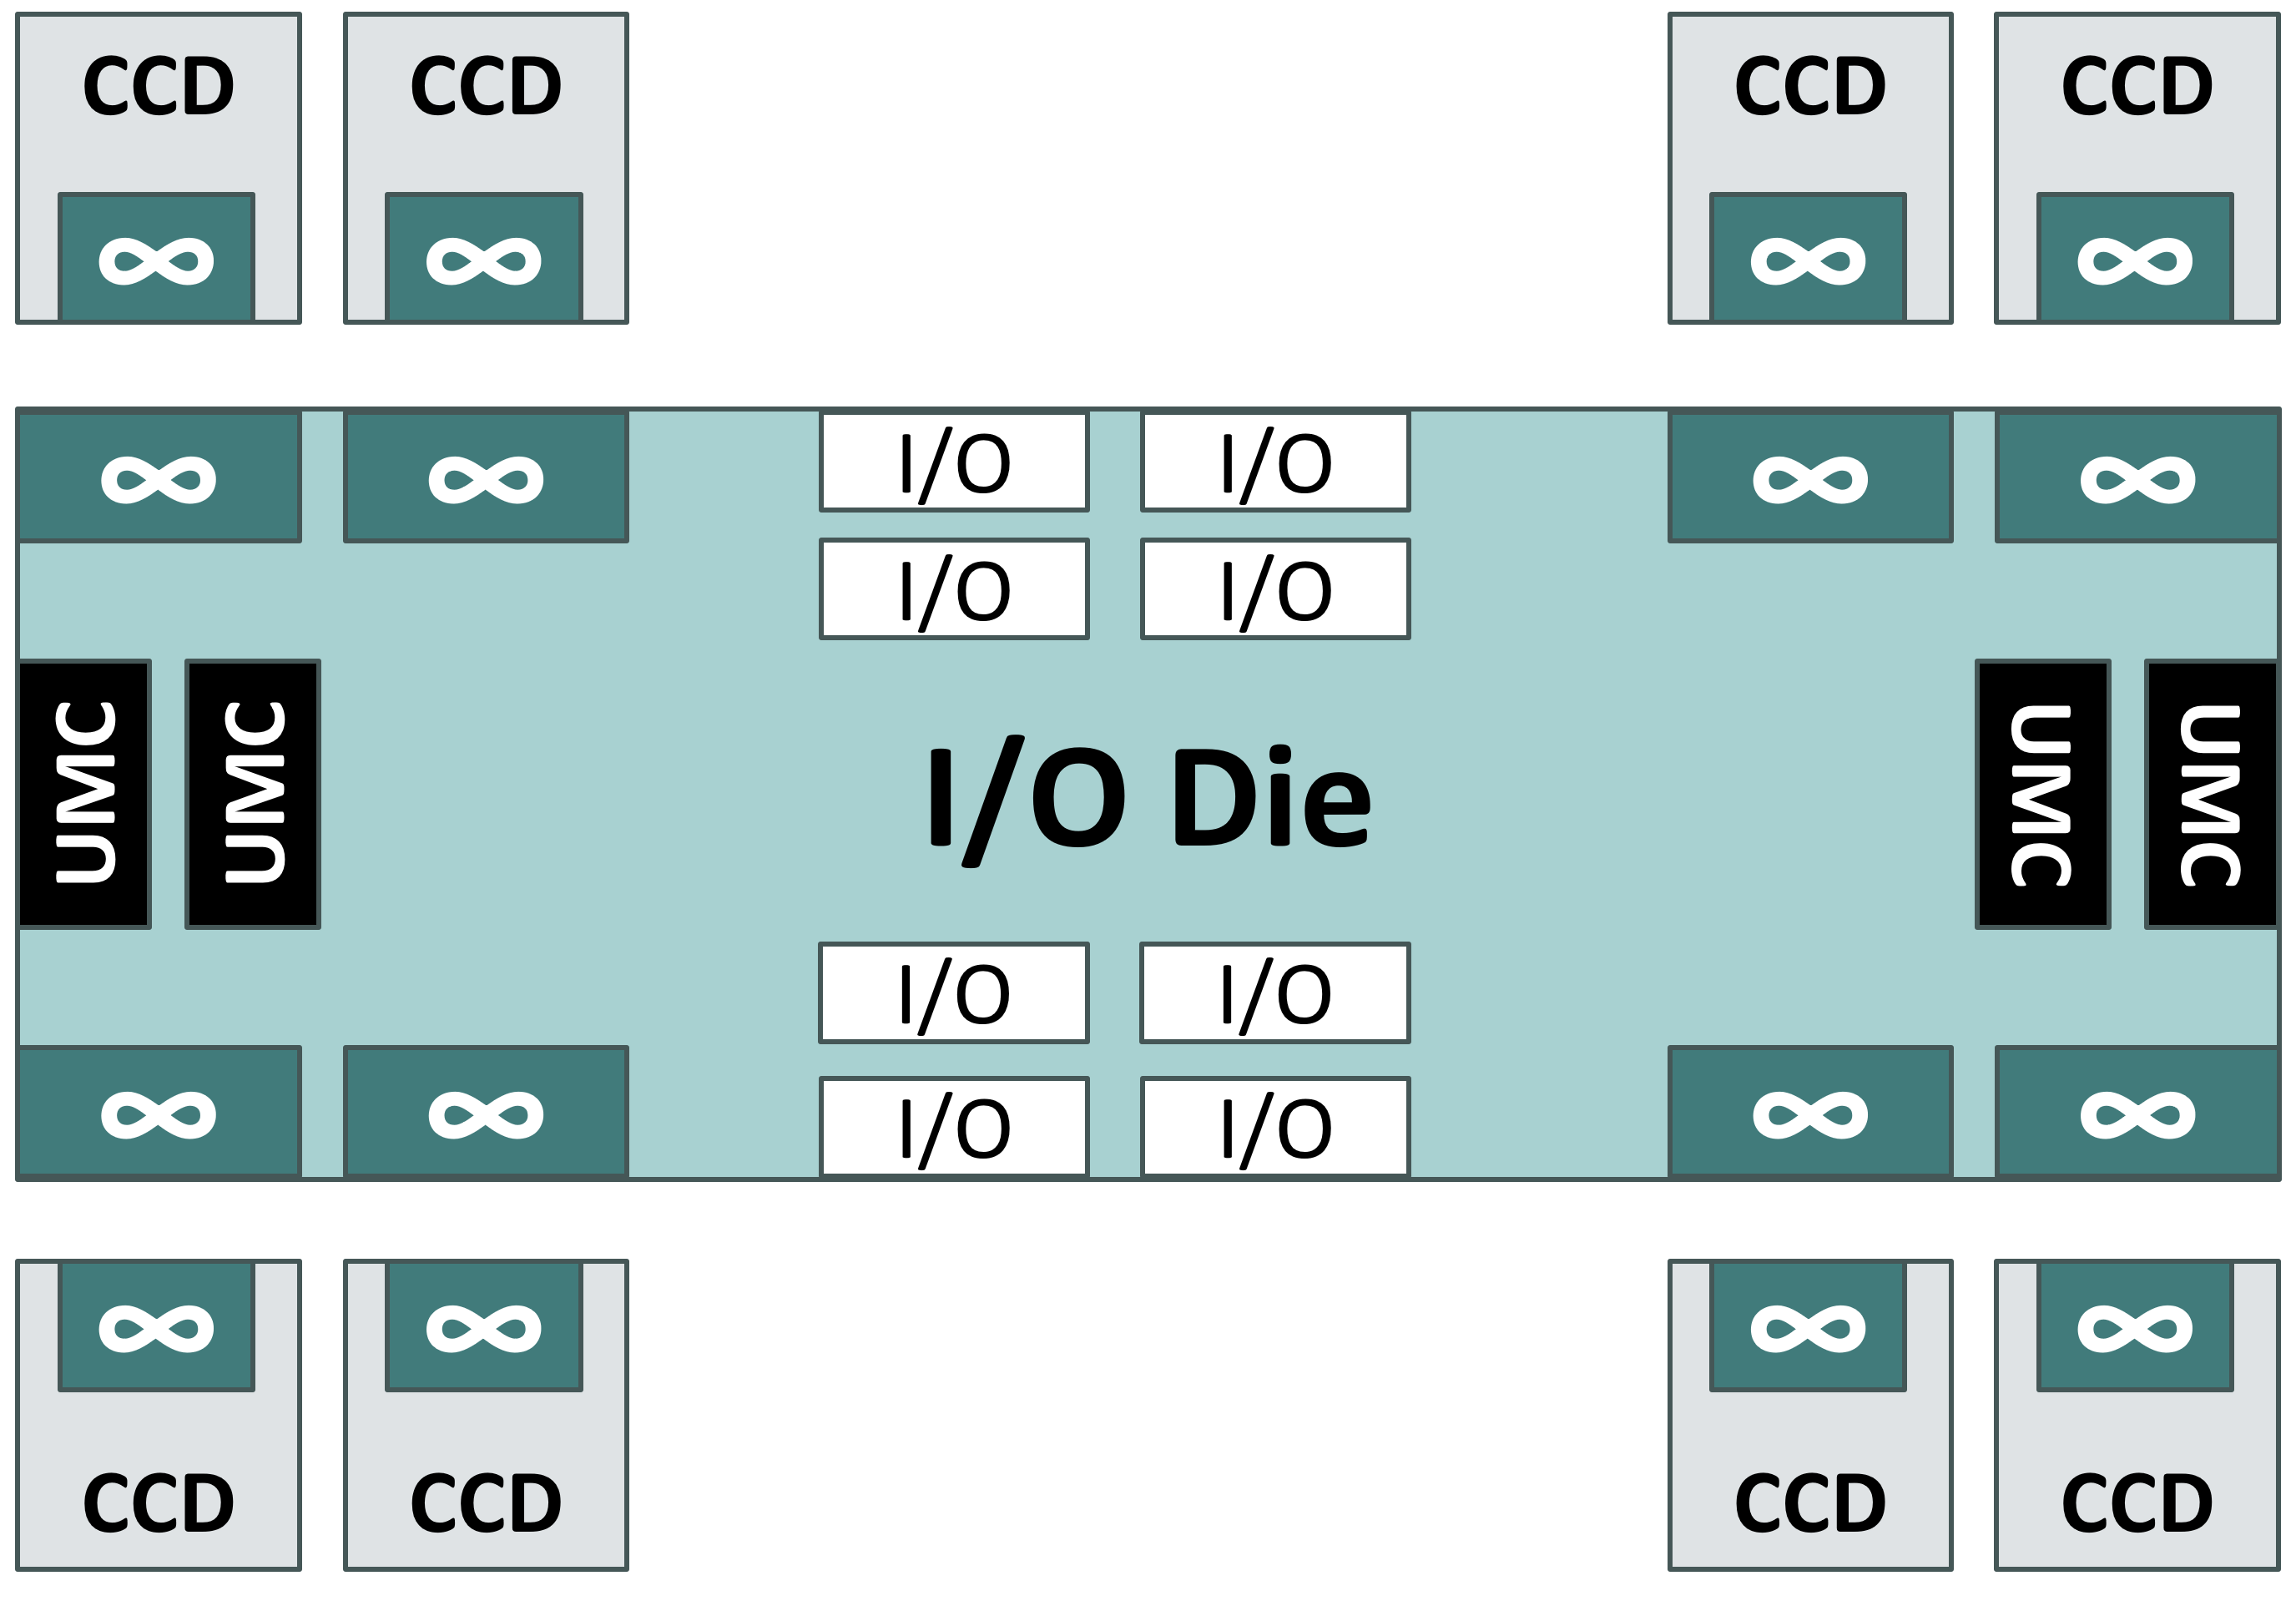
\includegraphics[width=\columnwidth]{figures/background/amd_arch/processor.png}
    \caption{AMD EPYC Zen 3 Architecture - CPU}
    \label{fig:amd-cpu}
\end{figure}


\Cref{fig:amd-cpu} shows a high-level overview of the architecture of the AMD EPYC Zen 3 processors.
The figure shows the following components:
\textbf{1) I/O:} The component that handles the input-output from the peripheral devices. This is where the PCIe communication happens.
\textbf{2) UMC:} The Unified Memory Controller is the controller that communicates with the DRAM.
\textbf{3) CCD:} The Core Complex Dies are where the cores (execution units) and caches reside.
\textbf{4) Infinity Fabric ($\infty$):} The interconnect that connects all of the components within the AMD CPU.

\subsubsection{CPU Pipelines}
\label{subsubsec:cpu-pipelines-bg}

Modern CPUs rely on executing multiple instructions simultaneously to maximise performance.
To achieve this, the CPUs have a multi-stage pipeline with the following stages: 1) Fetch, 2) Decode, 3) Schedule and Execute and 4) Retire.
We provide a simplified view of the pipeline in the CPU cores of the AMD EPYC Zen 3 processors in \Cref{fig:amd-core} and a brief description of each of the stages below:\\
\textbf{Fetch: } This stage fetches the next macro-op from the cache or the memory. 
However, the next macro-op to be fetched may not be deterministic, given the program may contain branches. 
In such cases, this stage also uses branch prediction to speculate on which instruction may be executed next and fetch that instruction.\\
\textbf{Decode: } This stage involved decoding the fetched macro-op into one or more micro-ops, which are then forwarded to the next stages.\\
\textbf{Schedule and Execute: } The scheduler(s) determine which instruction can be executed next based on the availability of the data that the instruction requires. 
This ensures that a long-running instruction (e.g., where the data is unavailable) does not stall all other independent instructions that can be executed.
As such, instructions here can be executed out of program order. 
Once the instruction has finished execution and the output of the instruction (if any) is available in the registers, the instruction is removed from the scheduler. 
\footnote{On AMD Zen 3 architecture, each scheduler has a capacity of 24 entries.}
As load and store are common but time-consuming instructions, this stage also consists of a load-store queue where pending load and store operations are held. \\
\textbf{Retire: } This stage ensures that instructions are retired in the program order so that the program can remain oblivious to the out-of-order execution that occurred in the previous stage.

\begin{figure}[!htb]
    \centering
    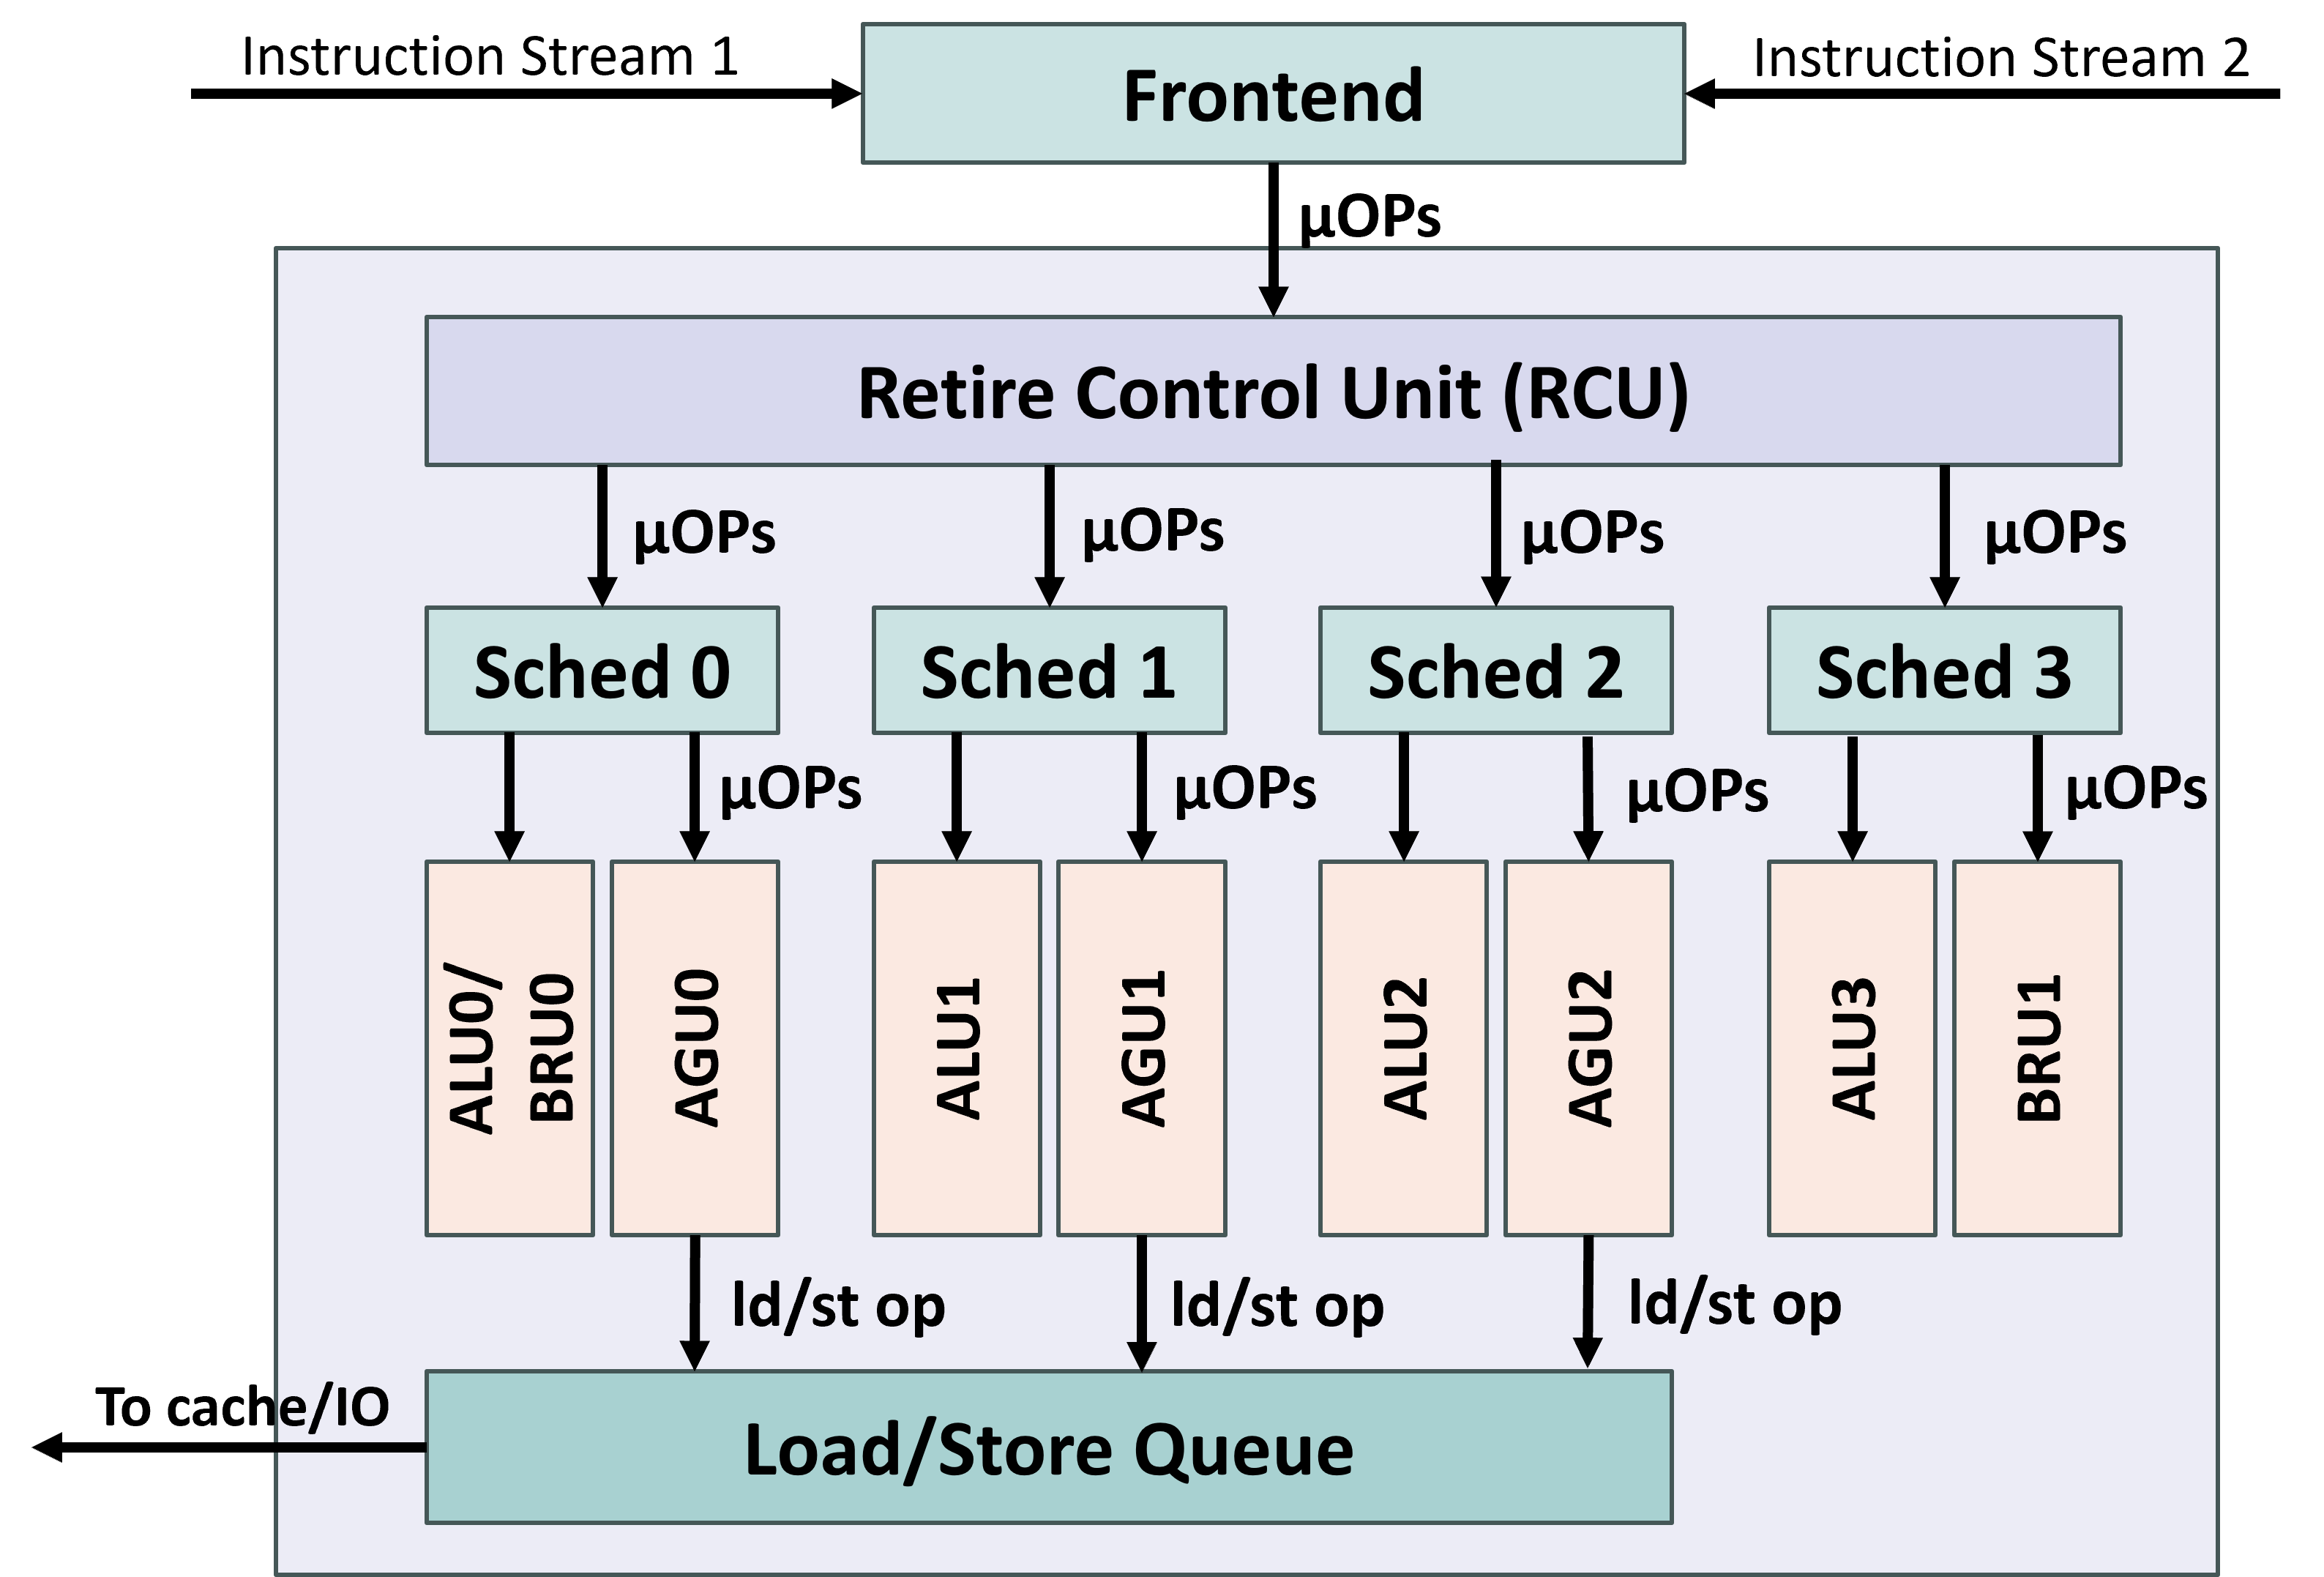
\includegraphics[width=\columnwidth]{figures/background/amd_arch/core.png}
    \caption{AMD EPYC Zen 3 Architecture - Core}
    \label{fig:amd-core}
\end{figure}

\subsubsection{PCIe transactions to/from CPU}

A program running on the CPU can transfer data to the PCIe device/endpoint in two major ways: 1) Memory operations via memory-mapped IO (MMIO) and 2) Direct memory access (DMA).
MMIO enables the CPU to map some memory region of the PCIe endpoint in the CPU's physical address space.
Any process with the proper permissions can then map this memory within the process and perform normal \textit{load} or \textit{store} operations on this memory.
However, this approach requires the execution units of the CPU to issue repeated \textit{load/store} instructions to copy data to the PCIe endpoint.
While this method is useful for reading or writing limited content, such as small configuration parameters, to the PCIe endpoints, it is inefficient for transferring a large amount of data.
To alleviate this, a lot of PCIe endpoints consist of a special hardware component called a DMA engine.
The DMA engine can copy large chunks of contiguous data without involving the execution units of the CPU.

For MMIO-based transactions, the load or store instructions go through the same instruction pipeline outlined in \Cref{fig:amd-core}. 
From the Load Store Queue, they end up in the I/O die outlined in \Cref{fig:amd-cpu} and go out the I/O block to the connected PCIe endpoint.
For DMA transactions (usually initiated by the PCIe endpoint), the transaction comes into the I/O block and, after some address and protocol translations, is sent out to the DRAM via the UMC.

\endinput


% \subsection{Threat Model}\label{subsec:interconnect-sc-threat-model}

\endinput
\chapter{NetShaper: A Differentially-Private Side Channel Mitigation System}

NetShaper \cite{sabzi2024netshaper} is both the name of the framework and the system that implements the framework to mitigate network side-channel attacks in internet applications.
We have provided a brief outline of the framework in \Cref{sec:netshaper-framework-bg}. 
Here, we describe the NetShaper system.

We first outline the requirements that the system should fulfil.
First, in any given window $W$, the system should be able to obtain the size of the payload in the buffering queue, with noise added to it. 
That is, the system should be able to complete the execution of $f_{DP}(S, t_{start}, t_{start} + W)$.
In the same window, the system should also be able to send out the payload, with padding, if necessary, such that the total data sent out, $b_{out}$, is equal to the noised size. 
However, it is sufficient to be able to queue $b_{out}$ bytes to be sent out, even if the actual transmission goes beyond the window $W$, as long as any delays were not caused by the payload coming in or already present in the buffering queue. 
The reason for this is the post-processing property of DP that we outlined in \Cref{subsec:dp-bg}.

Second, the payload and the padding should be indistinguishable to any observer observing the outbound packet stream.
Hence, the payload and padding should both be subject to the same congestion control, re-transmission, loss recovery, and other network behaviour.
In addition, the outbound transmission should provide the same or a higher level of reliability than the applications using this system expect.

Finally, the system should be modular so that modifications to any one sub-component do not require changes in the other components.
The system should also be portable and easily deployable, requiring none to minimal changes on the end hosts where the applications are running.
These goals ascertain that the system is easy to adopt and deploy and can easily be modified per the deployer's requirements.


% 1. Complete DP measurement within the window W
% 2. Data and Dummy should be indistinguishable
% 3. Should provide the same level of reliability the application expects
% 4. Should be modular for easy modification to sub-components
% 5. Should be portable and easily deployable, with minimal modifications of the end-hosts.

\section{Proxy Architecture}
\label{sec:proxy-arch}

\begin{figure}[!htb]
    \centering
    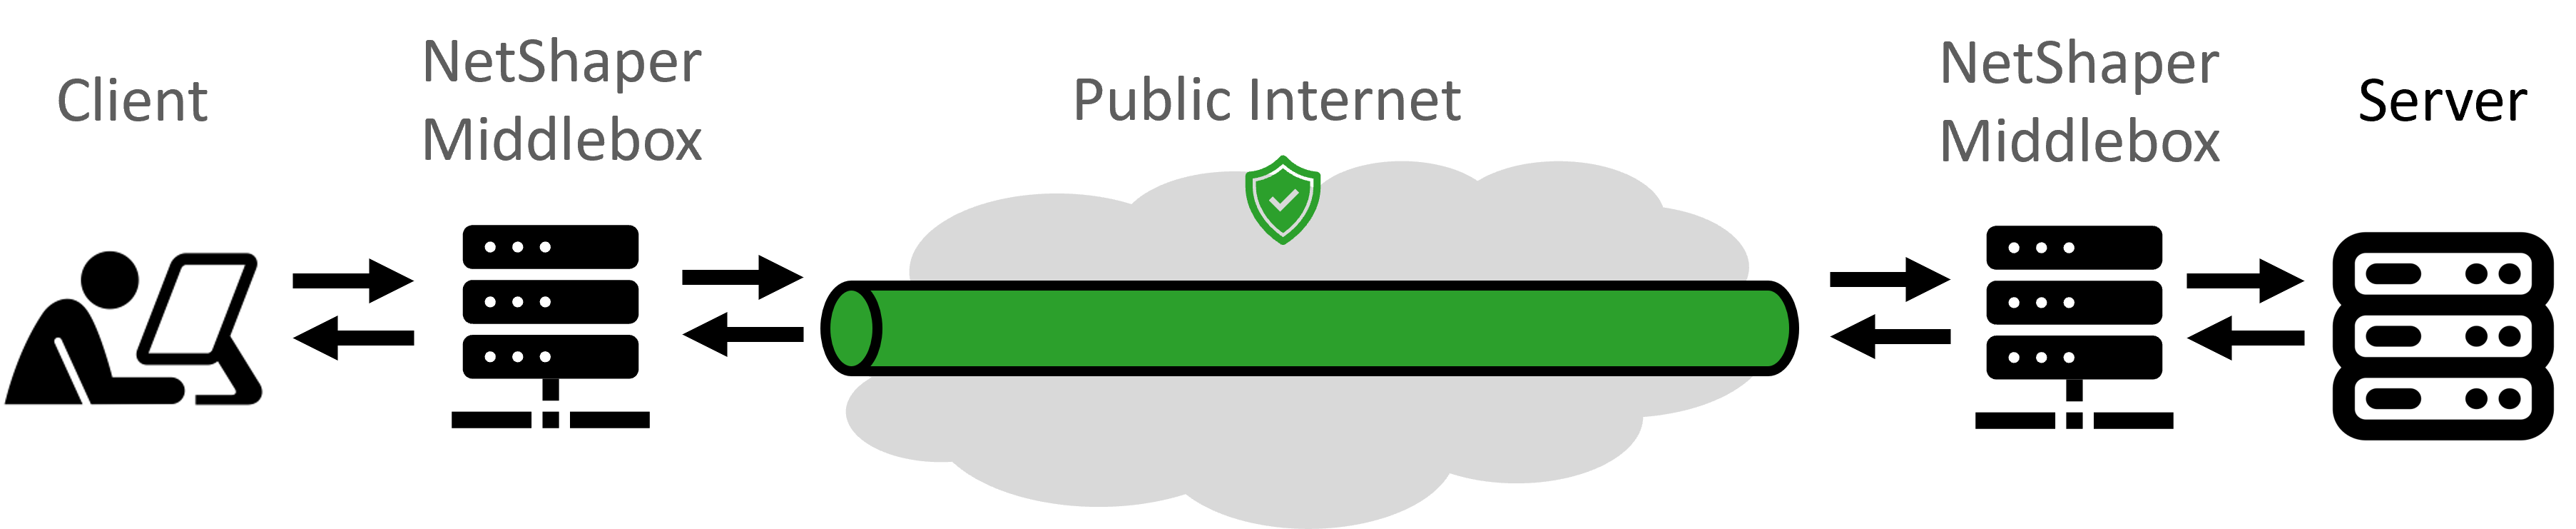
\includegraphics[width=\columnwidth]{figures/netshaper/netshaper-setup.png}
    \caption{NetShaper's Tunnel Setup}
    \label{fig:netshaper-setup}
\end{figure}

We designed NetShaper as a modular system that can be deployed using a pair of middleboxes, forming a forward and reverse proxy pair (see \Cref{fig:netshaper-setup}). 
Here, we describe in detail the architecture of the proxy setup and defer the discussion regarding the design of the middlebox to \Cref{sec:mb-design}. 

When using NetShaper, all clients communicate with the servers using three piecewise connections: 
(\textit{i}) between the client and the client-side middlebox, 
(\textit{ii}) between the client-side middlebox and the server-side middlebox, and
(\textit{iii}) between the server-side middlebox and the server.

For connection \textit{i} and \textit{iii}, NetShaper relies on standard TCP/UDP protocols. However, for connection \textit{ii} (i.e. to proxy the payload), NetShaper utilises QUIC. 
Using QUIC to proxy the payload avoids the TCP meltdown problem [??] that occurs when tunnelling TCP via TCP.
In addition, using QUIC also avoids the problem of an observer/attacker being able to distinguish between payload and padding that would occur when TCP was tunnelled via UDP (as the end host would retransmit payload, but the padding would not be retransmitted).

\paragraph{Setup.}
In order to be able to proxy end host traffic via NetShaper, the middleboxes need to be configured. 
The middleboxes first establish an encrypted QUIC connection between them, with user-specified reliability semantics.
Once the QUIC connection is established, NetShaper initialises three types of QUIC streams: Control, Data (Payload), and Dummy (Padding).
One \textit{control} stream is used to transmit messages regarding connection establishment or termination by the end host.
One \textit{dummy} stream is used for adding padding to the payload whenever necessary, based on the output of $f_{DP}$
\footnote{We avoid the use of PADDING frames in QUIC as they do not elicit acknowledgements and hence are distinguishable from the payload \cite{quic_rfc}.}.

\paragraph{Supporting multiple end hosts.}
As we discussed in \Cref{sec:quic-bg}, QUIC supports multiple streams in the same connection.
Using this, NetShaper can proxy the payload of multiple end hosts through a single QUIC connection between a pair of middleboxes.

While QUIC can support arbitrary initialisation and termination of streams, each stream has an associated header, which would increase the total transmission size.
For example, when transmitting two bytes in a single stream, the total transmission size would be $2 + S_{header}$.
However, when transmitting two streams of one byte each, the total transmission size would be $2 + 2*S_{header}$. 
An adversary may be able to distinguish between these two scenarios.
In order to avoid such a situation, NetShaper fixes and initialises a fixed number of streams per QUIC connection during the setup phase.
NetShaper assigns an unused stream to the client whenever a new client connects to the middlebox.
Similarly, NetShaper marks a stream as unused when an end host terminates the connection.

\endinput
\section{Middlebox Design}
\label{sec:mb-design}

While it is possible to apply NetShaper framework's approach at any network layer, we chose to develop the system as an L4 (Transport Layer) proxy.
This enables the system to be easily deployable, entirely in userspace and without requiring any superuser privileges. 
Developing NetShaper at L2 (Data Link Layer) or L3 (Network Layer) would require the deployer to either have the ability to modify the OS kernel or deploy some form of kernel bypass.

\begin{figure}[!htb]
    \centering
    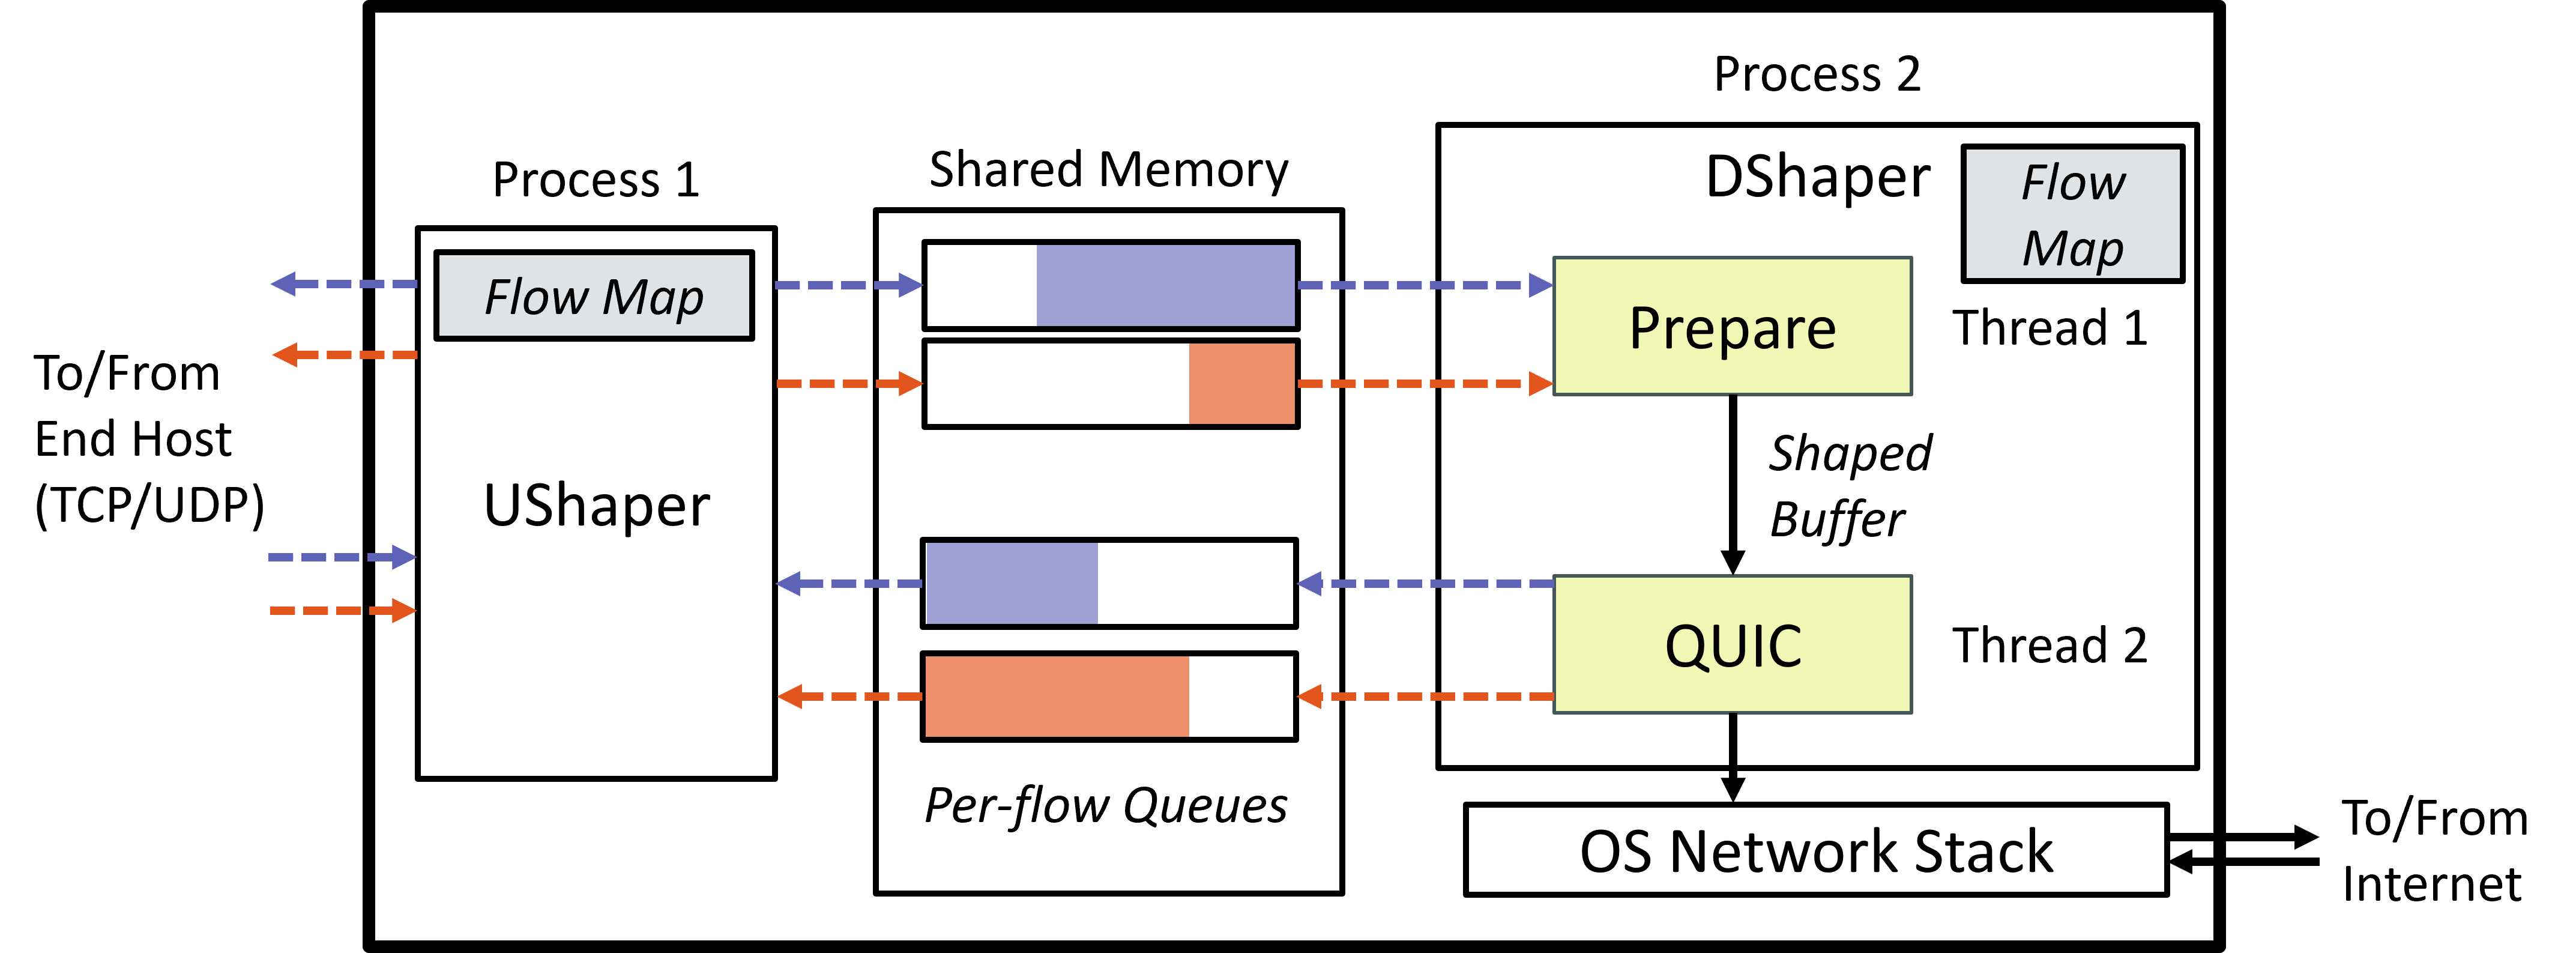
\includegraphics[width=\columnwidth]{figures/netshaper/middlebox-design.png}
    \caption{NetShaper Middlebox Design}
    \label{fig:middlebox-design}
\end{figure}

As outlined in \Cref{fig:middlebox-design}, NetShaper's middlebox consists of two main processes: UShaper and DShaper, and a shared memory between them.

\paragraph{UShaper.}
The \textit{UShaper} implements a client or a server to communicate with the end host.
It shares some Lamport Queues (LQs) [??] with DShaper.
It also consists of a flow map that maps a client with a corresponding pair of LQs.
\textit{UShaper} updates the flow map whenever a client establishes or terminates a connection.
In addition, it assigns an unused pair of LQs (one outbound and one inbound) to a new client and revokes that whenever the client terminates the connection.
The \textit{UShaper} receives outbound traffic from the end host and enqueues the payload in the assigned LQ.
Similarly, it dequeues inbound traffic from the inbound LQs and sends it to the corresponding end hosts.

\paragraph{DShaper.}
The \textit{DShaper} consists of two threads: \textit{Prepare} and \textit{QUIC worker}, and a flow map.
The flow map maps an LQ with a pre-initialised QUIC stream.
The \textit{Prepare} thread also measures the data available in the outbound LQs at the start of the window $W$.
It then adds noise to this available size based on the DP parameters.
Finally, it enqueues the payload and padding that needs to be transmitted.
The \textit{QUIC worker} transmits the enqueued data out to the network.
It also processes the received data, places it in the relevant LQ, and updates the flow map whenever a client initialises or terminates a connection.

In order to ensure that the operation of \textit{UShaper}, \textit{Prepare}, and \textit{QUIC worker} do not interfere with each other, we apply a few constraints in the implementation, and during the deployment of NetShaper.
First, all three components are required to be pinned on separate cores so that the execution time of one may not impact the others.
Second, in order to not leak the size of the payload due to the processing time of the enqueue operation done by the \textit{Prepare} thread, the \textit{Prepare} thread applies a lock for a fixed duration, during which the \textit{QUIC worker} can not transmit the data. 
We have outlined pseudo-code for both prepare and QUIC worker in \Cref{lst:prepare_and_worker}.
Finally, when receiving data, the \textit{QUIC worker} also enqueues the dummy bytes to a designated LQ so that the processing time remains consistent with the size of the data (see Figure ??).

\paragraph{Shared Memory.}
Both \textit{UShaper} and \textit{DShaper} have a shared memory between them.
This shared memory consists of three types of LQs: Control, Payload, Dummy
Similar to the stream types outlined in \Cref{sec:proxy-arch}, \textit{Control} LQ transmits the information about a connection establishment or termination by a client. 
\textit{Payload} LQ consists of the bytes received from the end host or to be sent to the end host.
\textit{Dummy} LQ consists of the dummy/padding bytes that are received.

\begin{minipage}{\textwidth}
\lstinputlisting[language=Python]{code/netshaper/prepare_and_worker.py}
\captionsetup{type=lstlisting}
\caption{Prepare and QUIC Worker Pseudo-code}
\label{lst:prepare_and_worker}
\end{minipage}

\endinput


\begin{figure}[!htb]
    \centering
    
\includegraphics[width=\columnwidth]{figures/netshaper/middlebox-design-overview.png}
    \caption{Overview of NetShaper's Middlebox}
    \label{fig:middlebox-design-overview}
\end{figure}

\endinput

Should we add pseudo-codes for UShaper and DShaper?
\section{Performance}\label{sec:netshaper-performance}
\section{Limitations and Discussion}\label{sec:netshaper-discussion}

\endinput
\chapter{Side Channel Attacks in Interconnects}

This chapter describes some avenues that can be used to carry out a side-channel attack on interconnects like PCIe and the challenges in pursuing those approaches.
In order to carry out a side-channel attack on PCIe, the first obvious step is to be able to transmit some data on the interconnect.
There are two major ways to achieve this: loads/stores on PCIe memory or configuration mapped to the CPU's address space or using DMA from the PCIe device to copy data to/from the CPU memory.
We describe the first approach in \Cref{sec:contention-with-stores}, and the second approach in \Cref{sec:contention-with-cudamemcpy}.


\section{Creating contention with load/store instructions}
\label{sec:contention-with-stores}

We have outlined the types of transactions PCIe supports in \Cref{tab:pcie-transaction-types}.
Most PCIe transactions are non-posted and, hence, are synchronous.
The synchronous behaviour enforces that no two load/store (i.e. read or write) operations to the same PCIe region can be issued in parallel.
However, having multiple parallel transactions that are in flight at the same time is necessary for the attacker to always have one pending packet in the PCIe buffer targeted for the side-channel attack
\footnote{An attacker can measure the delay in the transmission of that packet and infer the presence or absence of the victim traffic}.
As such, the attacker can only rely on non-posted transactions, and in particular, memory write operations
\footnote{While messages are also non-posted, they are usually generated by the underlying hardware directly, and the user has no control over those messages}.

In order to generate memory writes from the CPU, the attacker can map the device memory of a PCIe device, like a GPU, to an application running on the CPU and then issue store operations on that mapped memory.
Multiple store operations can be asynchronously issued on most modern processors as they support out-of-order execution. 
However, the same out-of-order execution feature makes it difficult for the attacker to accurately measure a store operation's time since the timer instruction can also be executed out of order.
In order to measure time accurately, most applications rely on issuing a fence instruction
\footnote{A fence instruction imposes ordering constraints, thus ensuring that any instruction after the fence is not executed before \textit{all} instructions before the fence are executed}.
However, this solution would not work for the attacker as the fence would not allow the next store instruction to be issued in parallel to the previous one, negating the benefit of using a posted (async) transaction.


\subsection{Measuring time of async stores}
\label{subsec:async_store_time}

In order to measure the completion time of a store operation which is issued out-of-order, we make use of two key insights:

\textit{First}, the CPU core would need to keep track of all instructions executed out-of-order so that they are retired in program order.
Keeping this track would require a scheduler and a buffer in the hardware, which would have a limited and fixed size.
The AMD CPU has four schedulers as described in \Cref{subsubsec:cpu-pipelines-bg}. Each scheduler has a fixed number of instruction slots $size_{sched}$.
In addition, for tracking load and store operations that are in flight, the CPU also has an LSQ, with a fixed number of slots for loads ($size_{ldq}$) and for stores ($size_{stq}$).
So, if the total number of pending (in flight) store instructions is larger than the total size of the scheduler slots and the store queue, the next instruction will be blocked, until one (or more) of the previous instructions finishes.

\textit{Second}, it is sufficient for the attacker to know if \textit{a} store instruction was delayed, and not if a particular store instruction was delayed.
% Convince why this is the case.
This would mean that we can use the first insight to queue a timer instruction immediately after issuing $size_{sched} + size_{stq}$ stores, and that timer will execute only after a store has completed.


\subsection{Evaluation}
\label{subsec:store-eval}

\endinput

\section{Creating contention with cudaMemcpy}
\label{sec:contention-with-cudamemcpy}

\section{Discussion}\label{sec:interconnect-sc-discussion}

\endinput

Should we consider the pre-microcode-update results and talk about that? It is NOT a vulnerability, just a behavioural observation. Hence, I don't think we need responsible disclosure
\chapter{Conclusion}

\section{Summary of Results}\label{sec:result-summary}
\section{Future Work}\label{sec:future-work}

\endinput


\begin{singlespace}
\raggedright
\bibliographystyle{abbrvnat}
\bibliography{biblio}
\end{singlespace}

\appendix
%    6. Appendices (including copies of all required UBC Research
%       Ethics Board's Certificates of Approval)
%\include{reb-coa}	% pdfpages is useful here
\chapter{Some Appendix}

\backmatter
%    7. Index
% See the makeindex package: the following page provides a quick overview
% <http://www.image.ufl.edu/help/latex/latex_indexes.shtml>


\end{document}
